%%%%%%%%%%%%%%%%%%%%%%%%%%%%%%%%%%%%%%%%%%%%%%%%%%%%%%%%%%%%%%%%%%%%%%%%%%%%%%%%%%%%%%%%%%%%%%%%%%
%%%%%%%%%%% Document class and package options
%%%%%%%%%%%%%%%%%%%%%%%%%%%%%%%%%%%%%%%%%%%%%%%%%%%%%%%%%%%%%%%%%%%%%%%%%%%%%%%%%%%%%%%%%%%%%%%%%%
\documentclass[a4paper,12pt]{report}

\usepackage{graphicx}
\usepackage{subcaption}
\usepackage{amsmath,amssymb,amsthm}
\usepackage{listings}
\usepackage{multicol}
\usepackage{enumerate}
\usepackage{enumitem}
\usepackage{fancyhdr}
\usepackage{longtable}
\usepackage{xcolor}
\usepackage{algorithm}
\usepackage{algorithmic}
\usepackage{booktabs}
\usepackage{multirow}
\usepackage{tabularx}
\usepackage{float}
\usepackage{tikz}
\usetikzlibrary{shapes.geometric, arrows.meta, positioning, fit, backgrounds, calc}

%%%%%%%%%%%%%%%%%%%%%%%%%%%%%%%%%%%%%%%%%%%%%%%%%%%%%%%%%%%%%%%%%%%%%%%%%%%%%%%%%%%%%%%%%%%%%%%%%%
% Include page set-up options
%%%%%%%%%%%%%%%%%%%%%%%%%%%%%%%%%%%%%%%%%%%%%%%%%%%%%%%%%%%%%%%%%%%%%%%%%%%%%%%%%%%%%%%%%%%%%%%%%%
\input{pagesetup.cfg}

%% ____Bibliography____%%
\usepackage[numbers,sort&compress]{natbib}
\usepackage{chapterbib}
\usepackage[breaklinks]{hyperref}
\hypersetup{colorlinks=true,citecolor=blue,linkcolor=blue,urlcolor=blue}

%% ____URL formatting____%%
\usepackage{url} 
\def\UrlBreaks{\do/}

%% ____Code listing style____%%
\definecolor{codebg}{RGB}{247,249,251}
\definecolor{codekw}{RGB}{41,65,122}
\definecolor{codecm}{RGB}{110,120,130}
\definecolor{codestr}{RGB}{50,120,50}
\lstset{
  basicstyle=\ttfamily\small,
  keywordstyle=\color{codekw}\bfseries,
  commentstyle=\color{codecm}\itshape,
  stringstyle=\color{codestr},
  backgroundcolor=\color{codebg},
  breaklines=true,
  frame=single,
  rulecolor=\color{codekw!30},
  framesep=5pt,
  aboveskip=8pt,
  belowskip=8pt,
  captionpos=b,
  showstringspaces=false,
  columns=fullflexible,
  numbers=left,
  numberstyle=\tiny\color{gray},
  numbersep=8pt
}

%% ____Theorem-like environments____%%
\theoremstyle{definition}
\newtheorem{definition}{Definition}[chapter]
\newtheorem{property}{Property}[chapter]
\theoremstyle{plain}
\newtheorem{theorem}{Theorem}[chapter]

%% ____Custom math commands____%%
\newcommand{\Poseidon}{\mathsf{Poseidon}}
\newcommand{\field}{\mathbb{F}_p}

\begin{document}
	
%%%%%%%%%%%%%%%%%%%%%%%%%%%%%%%%%%% The Front Matter %%%%%%%%%%%%%%%%%%%%%%%%%%%%%%%%%%%%
% Title Page

\thispagestyle{empty}

\begin{center}

\begin{center}
 
\includegraphics[width=2cm,keepaspectratio=true]{Front_matters/uor_logo.jpg}
 % uor_logo.jpg: 236x331 pixel, 72dpi, 8.33x11.68 cm, bb=0 0 236 331
\end{center}

\vspace{1.5cm}
\begin{huge}
%%%%%%%%%%%%%%%%%%%%%%%%%%%%%%%%%%%%%%%%%%%%%%%%%%%%
% Project title
%%%%%%%%%%%%%%%%%%%%%%%%%%%%%%%%%%%%%%%%%%%%%%%%%%%%
Privacy-Preserving Electronic Voting Using Zero-Knowledge Proofs on a Custom Blockchain
%%%%%%%%%%%%%%%%%%%%%%%%%%%%%%%%%%%%%%%%%%%%%%%%%%%%
\end{huge} \\
\vspace{1cm}

\begin{normalsize}
An undergraduate project report submitted to the
\end{normalsize}\\
\vspace{1cm}

\begin{large}
Department of Electrical and Information Engineering\\
Faculty of Engineering\\
University of Ruhuna\\
Sri Lanka
\end{large}\\

\vspace{1cm}

\begin{normalsize}in partial fulfillment of the requirements for the \end{normalsize}\\
\vspace{1cm}

\begin{large}\textbf{Degree of the Bachelor of the Science of Engineering Honours}\end{large}\\

\vspace{1cm}
\begin{normalsize}by  \end{normalsize}
\vspace{1cm}

\begin{tabular}[h]{lll}
 %%%%%%%%%%%%%%%%%%%%%%%%%%%%%%%%%%%%%%%%%%%%%%%%%%%%%%%%%%
 % Names and Registration Numbers
 %%%%%%%%%%%%%%%%%%%%%%%%%%%%%%%%%%%%%%%%%%%%%%%%%%%%%%%%%%
 K.K.R. Kumarasinghe	& - & 	EG/2021/4632\\
 R.M.D. Madhusankha	& - & 	EG/2021/4655\\
 R.M.T. Pradeepani	& - & 	EG/2021/4725\\
 K.K.M.P. Ranasinghe 	& - &	EG/2021/4735
 %%%%%%%%%%%%%%%%%%%%%%%%%%%%%%%%%%%%%%%%%%%%%%%%%%%%%%%%%%
\end{tabular}\\
\vspace{1cm}

%\date{June, 2009}
\vspace{1cm}

%%%%%%%%%%%%%%%%%%%%%%%%%%%%%%%%%%%%%%%%%%%%%%%%%%%%%%
% if one supervisor
%%%%%%%%%%%%%%%%%%%%%%%%%%%%%%%%%%%%%%%%%%%%%%%%%%%%%%%
%  .............................................. \\
% Prof. A.B.C. Dee\\
% (Supervisor)


%%%%%%%%%%%%%%%%%%%%%%%%%%%%%%%%%%%%%%%%%%%%%%%%%%%%
% If two supervisors
%%%%%%%%%%%%%%%%%%%%%%%%%%%%%%%%%%%%%%%%%%%%%%%%%%%%
\begin{tabular}[h]{lll}

	\begin{tabular}{c}
	.............................................. \\
	Prof. A.B.C. Dee\\
	(Supervisor)
	\end{tabular}
&
	\begin{tabular}{c}
	.............................................. \\
	Prof. A.B.C. Dee\\
	(Co-Supervisor)
	\end{tabular}

\end{tabular}\\
% End of "If two supervisors


\end{center}

%%%%%%%%%%%%%%%%%%%%%%%%%%%%%%%%%%%%%%%%%%%%%%%%%%%%%%%%%%%%%%%%%%%%%%%%%%%%%%%%%%%%%%%%%%%%%%%%%%
% END OF FILE
%%%%%%%%%%%%%%%%%%%%%%%%%%%%%%%%%%%%%%%%%%%%%%%%%%%%%%%%%%%%%%%%%%%%%%%%%%%%%%%%%%%%%%%%%%%%%%%%%%


\renewcommand{\thepage}{\roman{page}}


\chapter*{Abstract}

Electronic voting systems must simultaneously guarantee eligibility verification, ballot privacy, end-to-end verifiability, and coercion resistance. This project presents a complete privacy-preserving e-voting platform that achieves \textit{voter--ballot unlinkability} through zero-knowledge proofs on a purpose-built, gasless blockchain.

A Noir arithmetic circuit over the BN254 scalar field proves voter membership in a Merkle commitment tree via the Poseidon hash function, verified on-chain by the UltraHonk proof system---without revealing voter identity. Authentication employs a three-factor protocol (OTP, biometric, hardware-backed PIN) on a native mobile application; the ballot is cast from an ephemeral wallet, making it cryptographically unlinkable to the registered identity.

The system models Sri Lanka's 160-division electorate with village-officer enrollment, on-chain national aggregation, and a custom Go blockchain embedding the Ethereum Virtual Machine---processing all transactions at zero cost to participants. Block production is distributed across four independently-operated validators, the electoral authority and three political parties, under a Byzantine fault tolerant protocol in which each validator re-executes a proposed block before signing it and a quorum of three signatures is required to commit: no single operator can halt the election or unilaterally determine its contents. A suite of four Solidity smart contracts implements the election state machine with five independent layers of on-chain fraud prevention.

On the custom blockchain, on-chain proof verification completes in under 5\,ms; on-device proof generation takes 15--30\,s via WebAssembly. The 54-test contract suite validates all election phases, access controls, and adversarial scenarios. Any observer can independently verify every proof and recompute the tally from public state, providing end-to-end verifiability without trusted intermediaries.

\addcontentsline{toc}{chapter}{Abstract}

\input{Front_matters/acknowledgements}
\addcontentsline{toc}{chapter}{Acknowledgements}

\tableofcontents
\addcontentsline{toc}{chapter}{Contents}

\listoffigures	
\addcontentsline{toc}{chapter}{List of Figures}

\listoftables
\addcontentsline{toc}{chapter}{List of Tables}

\chapter*{Acronyms}

\noindent \begin{tabular}{lcl}
BN254 & - & Barreto-Naehrig Curve (254-bit)\\
DRE & - & Direct Recording Electronic\\
E2E & - & End-to-End\\
EVM & - & Ethereum Virtual Machine\\
GN & - & Grama Niladhari (Village Officer)\\
HSM & - & Hardware Security Module\\
LeanIMT & - & Lean Incremental Merkle Tree\\
NIC & - & National Identity Card\\
OTP & - & One-Time Password\\
PBFT & - & Practical Byzantine Fault Tolerance\\
SRS & - & Structured Reference String\\
TEE & - & Trusted Execution Environment\\
ZK & - & Zero-Knowledge\\
ZKP & - & Zero-Knowledge Proof\\
zk-SNARK & - & Zero-Knowledge Succinct Non-Interactive Argument of Knowledge\\
\end{tabular} 



\addcontentsline{toc}{chapter}{Acronyms}


%%%%%%%%%%%%%%%%%%%%%%% The main matters %%%%%%%%%%%%%%%%%%%%%%%%

\chapter{Introduction}\label{ch:introduction}

Electronic voting represents one of the most challenging applications of modern cryptography: a system must simultaneously prove that a voter is eligible (accountability) while ensuring that no one---not even the system operators---can determine how that voter voted (privacy). This chapter establishes the context, formally defines the problem, and outlines our approach.

\section{Background}

\subsection{The Democratic Election Challenge in Sri Lanka}

Sri Lanka is a parliamentary democracy with a complex multi-tier electoral structure. National elections are conducted across 22 electoral districts containing 160 polling divisions, administered through approximately 14,000 Grama Niladhari (Village Officer) divisions, serving over 16 million registered voters.

The current paper-ballot system faces significant challenges: counting delays of 24--48 hours, high logistical costs, susceptibility to human error, limited accessibility for disabled or overseas citizens, and expensive recounting processes.

\begin{figure}[H]
\centering
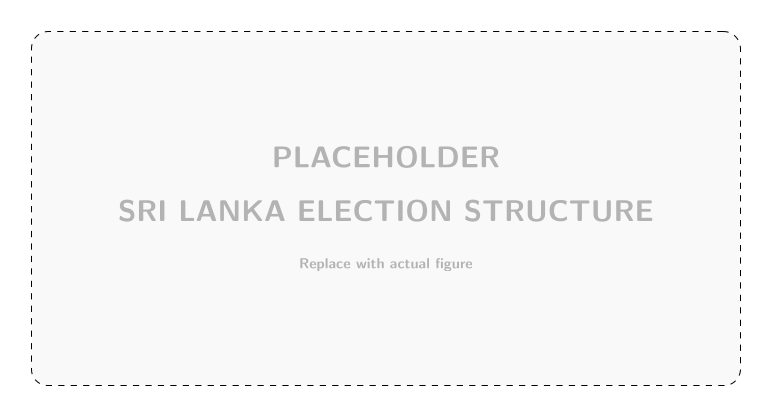
\includegraphics[width=0.85\textwidth]{Images/fig_sri_lanka_election_structure.png}
\caption{Sri Lanka's electoral hierarchy from the Election Commission down to 16+ million individual voters.}
\label{fig:sl-structure}
\end{figure}

\subsection{Formal Requirements for Secure Electronic Voting}

Any electronic voting system must satisfy four fundamental properties:

\begin{definition}[Eligibility Verification]
Only citizens on the certified register may vote; each may cast at most one ballot.
\end{definition}

\begin{definition}[Ballot Privacy]
No entity can determine how any specific voter cast their ballot.
\end{definition}

\begin{definition}[End-to-End Verifiability]
Any participant can verify that their ballot was recorded correctly and that the tally is correct.
\end{definition}

\begin{definition}[Coercion Resistance]
A voter cannot produce evidence proving how they voted to a third party.
\end{definition}

\subsection{Why Blockchain Alone Is Insufficient}

Blockchain provides integrity and transparency, but standard transactions reveal the sender address. On Ethereum, a vote transaction exposes: \texttt{From: 0xAlice To: Voting.sol Data: vote(3)}. If the address is linked to Alice's identity, ballot privacy is destroyed. Prior blockchain voting systems suffered this exact vulnerability.

\subsection{Zero-Knowledge Proofs: The Key Enabler}

Zero-knowledge proofs resolve the eligibility--privacy tension. Instead of revealing identity, a voter proves: \textit{``I am SOME valid registered voter''} without revealing which one. Combined with an ephemeral wallet for submission, this achieves cryptographic unlinkability between voter and ballot.

\begin{figure}[H]
\centering
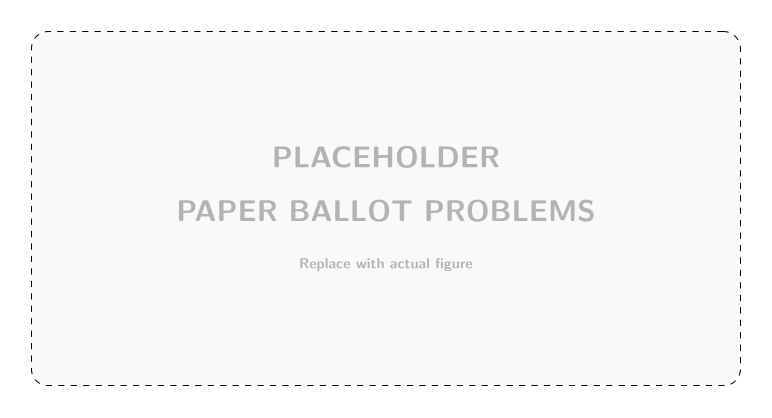
\includegraphics[width=0.85\textwidth]{Images/fig_paper_ballot_problems.png}
\caption{Paper ballot challenges and how our ZK-based system addresses each.}
\label{fig:paper-problems}
\end{figure}

\section{Problem Statement}

\begin{enumerate}
    \item \textbf{Ballot--voter linkability}: Blockchain transaction senders reveal voter identity.
    \item \textbf{Centralized trust}: Systems like Helios/MACI require trusted intermediaries.
    \item \textbf{Administrative infidelity}: Prototypes ignore real government structures.
    \item \textbf{Economic barriers}: Gas fees exclude voters from participation.
    \item \textbf{Weak authentication}: Wallet-only auth provides no physical presence verification.
    \item \textbf{Sybil vulnerability}: No national-level identity de-duplication.
\end{enumerate}

\section{Objectives and Scope}

\subsection{Objectives}
\begin{enumerate}
    \item Design a ZK circuit proving voter membership without revealing identity.
    \item Develop smart contracts with five layers of on-chain fraud prevention.
    \item Build a custom gasless blockchain embedding the EVM.
    \item Develop a mobile app with hardware security and on-device proof generation.
    \item Implement web administration for Election Authority and GN officers.
    \item Model Sri Lanka's 160-division structure with on-chain national aggregation.
    \item Achieve formal voter--ballot unlinkability:
\end{enumerate}

\begin{equation}
\Pr\left[\mathcal{A}(\text{chain}) \to (\text{Voter}, \text{Ballot})\right] \le \frac{1}{|\mathcal{V}|} + \text{negl}(\lambda)
\label{eq:anon-intro}
\end{equation}

\subsection{Scope}
\textbf{In scope}: Complete voting pipeline, Android mobile app, web console, custom blockchain, 54-test suite, performance evaluation.

\textbf{Out of scope}: Full ballot secrecy (homomorphic tallying), formal verification (Lean 4), production deployment, iOS testing.

\section{Methodology Overview}

The project followed an iterative bottom-up methodology:
\begin{itemize}
    \item \textbf{Phase 1 (Nov 2025 -- Feb 2026)}: ZK circuit, smart contracts, proof system, test suite, web frontend.
    \item \textbf{Phase 2 (Mar -- Jul 2026)}: Custom blockchain, mobile app, three-factor auth, multi-division, integration.
\end{itemize}

\section{Team Contributions}

\begin{table}[H]
\centering
\caption{Team Member Responsibilities}
\label{tab:team}
\begin{tabular}{|l|l|p{6cm}|}
\hline
\textbf{Member} & \textbf{Reg. No.} & \textbf{Primary Responsibilities} \\
\hline
K.K.R. Kumarasinghe & EG/2021/4632 & Smart contracts, testing, deployment \\
\hline
R.M.D. Madhusankha & EG/2021/4655 & Custom Go blockchain, REST API \\
\hline
R.M.T. Pradeepani & EG/2021/4725 & ZK circuit, cryptographic design \\
\hline
K.K.M.P. Ranasinghe & EG/2021/4735 & Mobile app, web frontend, auth \\
\hline
\end{tabular}
\end{table}

\begin{figure}[H]
\centering
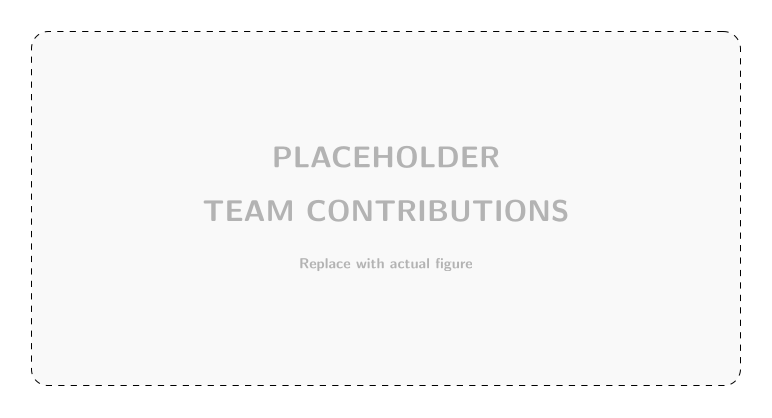
\includegraphics[width=0.75\textwidth]{Images/fig_team_contributions.png}
\caption{Team member contribution areas and overlap in integration work.}
\label{fig:team-contributions}
\end{figure}

\section{Report Organization}

The report is organized into 9 chapters covering the complete project from literature through implementation to evaluation.


\renewcommand{\thepage}{\arabic{page}}
\setcounter{page}{1}

\chapter{Literature Review}\label{ch:literature}

This chapter provides a comprehensive review of the theoretical foundations, prior electronic voting systems, blockchain-based voting proposals, and anonymous credential schemes that inform the design of our privacy-preserving voting system. We identify critical gaps in the existing literature and position our contribution within the broader landscape of cryptographic voting research.

\section{Theoretical Foundations}

\subsection{Zero-Knowledge Proofs}

A zero-knowledge proof (ZKP) is an interactive or non-interactive protocol between a prover $\mathcal{P}$ and a verifier $\mathcal{V}$ that enables $\mathcal{P}$ to convince $\mathcal{V}$ that a statement $x$ is true without revealing any information beyond the truth of the statement~\cite{goldwasser1989knowledge}.

\begin{definition}[Zero-Knowledge Proof System]
A proof system $(P, V)$ for a language $L$ is zero-knowledge if it satisfies:
\begin{enumerate}
    \item \textbf{Completeness}: If $x \in L$, then $\Pr[V \text{ accepts}] \geq 1 - \text{negl}(\lambda)$.
    \item \textbf{Soundness}: If $x \notin L$, then $\Pr[V \text{ accepts}] \leq \text{negl}(\lambda)$.
    \item \textbf{Zero-Knowledge}: $\exists$ simulator $S$ such that $\text{View}_V(P, V, x) \approx S(x)$.
\end{enumerate}
\end{definition}

The evolution from interactive to non-interactive zero-knowledge proofs (NIZKs) was enabled by the Fiat--Shamir heuristic~\cite{fiat1986prove}, which replaces the verifier's random challenges with hash function outputs. This transformation is critical for blockchain applications where the prover and verifier cannot interact in real-time.

\begin{equation}
\text{Fiat-Shamir}: \quad c = H(\text{transcript} \| \text{commitment})
\label{eq:fiat-shamir}
\end{equation}

\subsubsection{zk-SNARK Evolution}

The field of succinct non-interactive arguments of knowledge (zk-SNARKs) has evolved rapidly since Groth's seminal 2016 construction~\cite{groth2016size}:

\begin{table}[H]
\centering
\caption{Evolution of ZK proof systems relevant to voting applications.}
\label{tab:zk-evolution}
\begin{tabular}{|l|l|l|l|l|}
\hline
\textbf{System} & \textbf{Year} & \textbf{Trusted Setup} & \textbf{Proof Size} & \textbf{Verify Time} \\
\hline
Groth16 & 2016 & Per-circuit & 128 B & 1.5 ms \\
\hline
PLONK & 2019 & Universal (SRS) & 384 B & 5 ms \\
\hline
Halo2 & 2020 & None (IPA) & 5--10 KB & 200 ms \\
\hline
UltraHonk & 2023 & None (Keccak) & 2--4 KB & $<5$ ms \\
\hline
\end{tabular}
\end{table}

UltraHonk, developed by Aztec Labs as part of the Barretenberg library, represents the state-of-the-art for client-side proving. Its elimination of the trusted setup requirement makes it particularly suitable for voting systems where ceremony coordination presents logistical challenges~\cite{aztec2023ultrahonk}.

\begin{figure}[H]
\centering
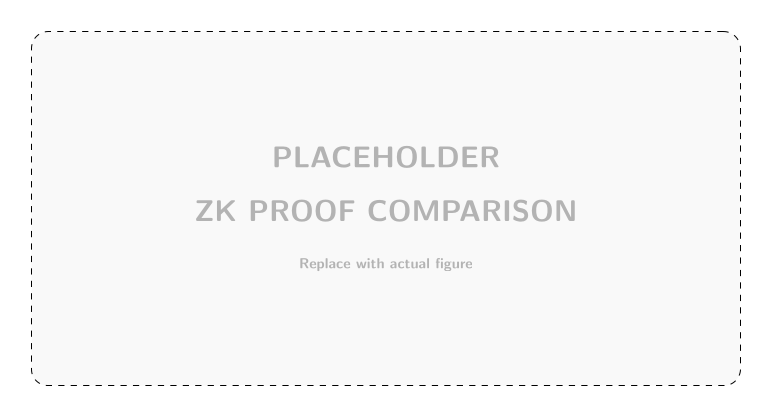
\includegraphics[width=0.85\textwidth]{Images/fig_zk_proof_comparison.png}
\caption{Comparative analysis of ZK proof systems across key dimensions: proof size, verification cost, setup requirements, and prover complexity.}
\label{fig:zk-comparison}
\end{figure}

\subsection{Poseidon Hash Function}

The Poseidon hash function~\cite{grassi2021poseidon} was specifically designed for arithmetic circuits over prime fields, making it orders of magnitude more efficient than algebraically-unfriendly hash functions like SHA-256 or Keccak when expressed as R1CS or Plonkish constraints.

\begin{definition}[Poseidon Permutation]
For a state width $t$ over a prime field $\mathbb{F}_p$, the Poseidon permutation $\pi: \mathbb{F}_p^t \to \mathbb{F}_p^t$ consists of:
\begin{enumerate}
    \item $R_f$ full rounds: $\text{ARK} \to \text{S-box}^t \to \text{MDS}$
    \item $R_p$ partial rounds: $\text{ARK} \to \text{S-box}^1 \to \text{MDS}$
    \item $R_f$ full rounds: $\text{ARK} \to \text{S-box}^t \to \text{MDS}$
\end{enumerate}
where the S-box is $x \mapsto x^\alpha$ with $\alpha = 5$ for BN254.
\end{definition}

The constraint cost comparison is dramatic:

\begin{table}[H]
\centering
\caption{Hash function constraint costs in BN254 arithmetic circuits.}
\label{tab:hash-constraints}
\begin{tabular}{|l|r|r|l|}
\hline
\textbf{Hash Function} & \textbf{Constraints} & \textbf{Ratio} & \textbf{Native to BN254?} \\
\hline
SHA-256 & $\sim$25,000 & 83$\times$ & No (bitwise) \\
\hline
Keccak-256 & $\sim$150,000 & 500$\times$ & No (bitwise) \\
\hline
MiMC & $\sim$730 & 2.4$\times$ & Yes \\
\hline
Poseidon ($t=3$) & $\sim$300 & 1$\times$ & Yes \\
\hline
\end{tabular}
\end{table}

For our system, we use two Poseidon variants:
\begin{align}
\Poseidon_1(x) &: \mathbb{F}_p \to \mathbb{F}_p \quad \text{(nullifier hash)} \\
\Poseidon_2(x, y) &: \mathbb{F}_p^2 \to \mathbb{F}_p \quad \text{(commitment, Merkle nodes)}
\end{align}

\subsection{Merkle Trees for Set Membership}

A Merkle tree~\cite{merkle1987digital} provides $O(\log n)$ proofs of set membership. Given a set of $n$ leaves $\{l_0, l_1, \ldots, l_{n-1}\}$, any leaf can prove membership by revealing only $\log_2 n$ sibling hashes along its authentication path.

\begin{equation}
\text{root} = H\left(H\left(H(l_0, l_1), H(l_2, l_3)\right), H\left(H(l_4, l_5), H(l_6, l_7)\right)\right)
\label{eq:merkle-root}
\end{equation}

The Lean Incremental Merkle Tree (LeanIMT)~\cite{semaphore2023lean} optimizes on-chain storage by only storing nodes along the ``frontier''---the rightmost path---reducing storage from $O(n)$ to $O(\log n)$ while maintaining the same root computation.

\begin{figure}[H]
\centering
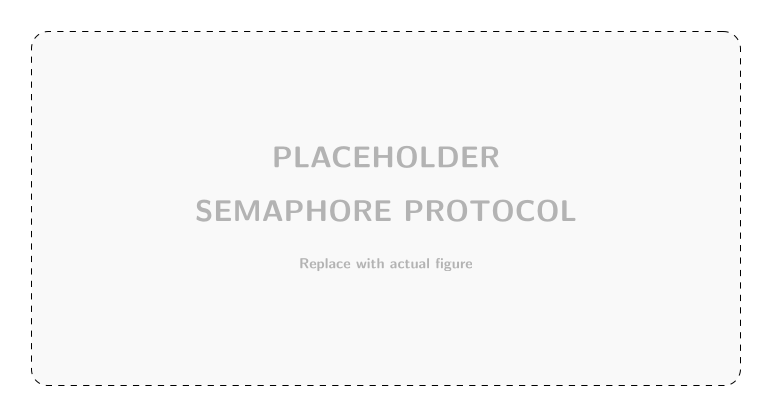
\includegraphics[width=0.85\textwidth]{Images/fig_semaphore_protocol.png}
\caption{Merkle tree membership proof: the prover reveals the path siblings (shaded) but not which leaf is theirs.}
\label{fig:merkle-membership}
\end{figure}

\subsection{BN254 Elliptic Curve}

The BN254 curve (also known as alt\_bn128 or bn256) is a Barreto--Naehrig pairing-friendly elliptic curve defined over a 254-bit prime field~\cite{barreto2005pairing}:

\begin{equation}
E: y^2 = x^3 + 3 \quad \text{over } \mathbb{F}_p
\end{equation}

where $p = 21888242871839275222246405745257275088696311157297823662689037894645226208583$.

The scalar field order (the field in which our circuit operates) is:
\begin{equation}
r = 21888242871839275222246405745257275088548364400416034343698204186575808495617
\end{equation}

BN254 is natively supported by the Ethereum Virtual Machine through precompiled contracts at addresses \texttt{0x06} (addition), \texttt{0x07} (scalar multiplication), and \texttt{0x08} (pairing check)~\cite{eip196,eip197}. This hardware-level support enables gas-efficient on-chain proof verification---a critical requirement for blockchain voting systems.

\section{Electronic Voting Systems: A Historical Perspective}

\subsection{First-Generation Systems (2005--2015)}

\begin{figure}[H]
\centering
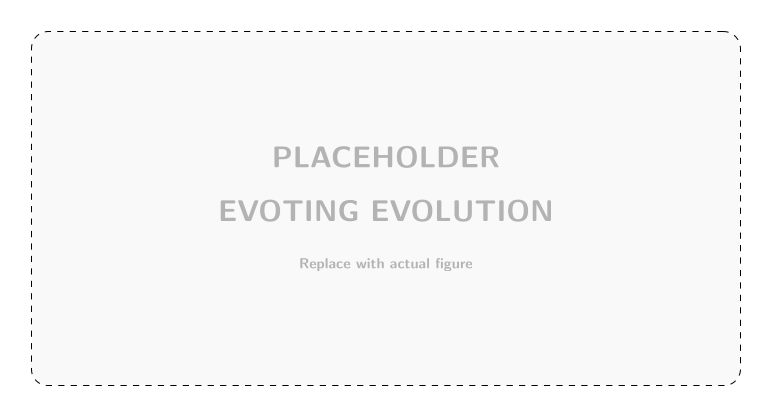
\includegraphics[width=0.85\textwidth]{Images/fig_evoting_evolution.png}
\caption{Evolution of electronic voting systems from centralized servers to blockchain-based privacy-preserving architectures.}
\label{fig:evoting-evolution}
\end{figure}

\subsubsection{Estonia's i-Voting (2005--Present)}

Estonia launched the world's first legally binding internet voting system in 2005~\cite{heiberg2012internet}. The system uses a double-envelope scheme:
\begin{enumerate}
    \item The voter signs their ballot with their national ID card (RSA-2048).
    \item A server strips the identity layer before tallying.
    \item Re-voting is permitted (last vote counts) as coercion mitigation.
\end{enumerate}

\textbf{Strengths}: Government-backed PKI, high adoption (51.1\% in 2023 elections), re-voting for coercion resistance.

\textbf{Weaknesses}: Server-side decryption creates a single point of failure~\cite{springall2014security}. An adversary with access to the collection server can deanonymize all votes. The system assumes trust in the election authority---precisely the assumption we aim to eliminate.

\subsubsection{iVote (New South Wales, Australia)}

The iVote system, deployed for state elections from 2011 to 2021, used a mix-net approach for anonymization~\cite{culnane2015verivote}. Voters authenticated via a PIN mailed to their registered address, then cast votes through a web interface. The system was retired after security researchers demonstrated that a TLS man-in-the-middle attack could modify votes in transit~\cite{halderman2015internet}.

\subsubsection{Swiss Post E-Voting}

Switzerland's Scytl-built system employed verifiable shuffles~\cite{haenni2017swiss} with individual verifiability codes. In 2019, a critical vulnerability was discovered in the decryption shuffle proof that could allow undetected vote manipulation~\cite{lewis2019swiss}. The system was suspended pending redesign.

\subsection{Second-Generation: Cryptographically Verifiable Systems}

\subsubsection{Helios (2008)}

Helios~\cite{adida2008helios} represents a landmark in verifiable voting. It uses ElGamal encryption with a mix-net for anonymization:

\begin{enumerate}
    \item Voter encrypts ballot: $c = \text{Enc}_{pk}(\text{vote}; r)$
    \item Encrypted ballot posted to public bulletin board
    \item Mix-net shuffles and re-encrypts
    \item Threshold decryption reveals tallied results
\end{enumerate}

\begin{figure}[H]
\centering
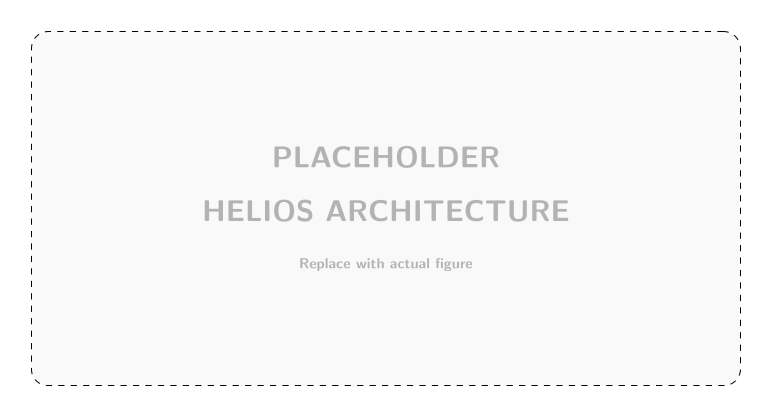
\includegraphics[width=0.85\textwidth]{Images/fig_helios_architecture.png}
\caption{Helios architecture: encrypted ballots are posted publicly, shuffled through a mix-net, and tallied via threshold decryption.}
\label{fig:helios-arch}
\end{figure}

\textbf{Limitations for our context}:
\begin{itemize}
    \item Requires trusted mix-net servers (at least one must be honest)
    \item No coercion resistance (voter can prove their vote via the ballot tracker)
    \item Not designed for blockchain integration
    \item Scalability issues with large electorates (16M+ voters)
\end{itemize}

\subsubsection{Belenios (2017)}

Belenios~\cite{cortier2017belenios} extended Helios with stronger verifiability properties but inherited the mix-net dependency. It introduced a credential-based approach where voters receive a private credential from a registrar, preventing ballot stuffing even if the voting server is compromised.

\subsection{Third-Generation: Blockchain-Based Voting}

\subsubsection{Voatz (2018--2020)}

Voatz deployed mobile blockchain voting in West Virginia (2018), Denver (2019), and several other jurisdictions for absentee military voters~\cite{voatz2020}. The system used a permissioned Hyperledger-based blockchain with biometric authentication.

\begin{figure}[H]
\centering
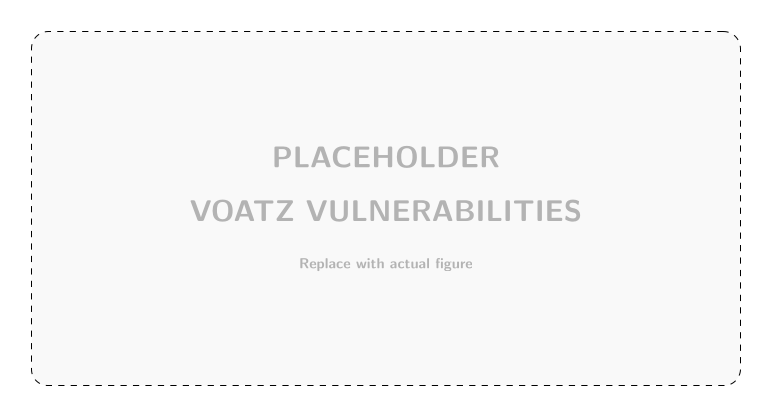
\includegraphics[width=0.85\textwidth]{Images/fig_voatz_vulnerabilities.png}
\caption{Security vulnerabilities identified in the Voatz system by MIT researchers, including the lack of end-to-end verifiability.}
\label{fig:voatz-vuln}
\end{figure}

In 2020, MIT researchers~\cite{specter2020ballot} identified critical vulnerabilities:
\begin{itemize}
    \item Server-side sees plaintext votes (no encryption)
    \item Biometric data transmitted to central server
    \item No end-to-end verifiability
    \item Client-side code obfuscated (prevents audit)
    \item Blockchain used only as append-only log (no cryptographic voting properties)
\end{itemize}

The Voatz case demonstrates that blockchain alone provides no ballot privacy---it merely records transactions transparently, making the privacy problem \textit{worse} unless cryptographic measures are added.

\subsubsection{McCorry et al. --- Open Vote Network (2017)}

McCorry, Shahandashti, and Hao~\cite{mccorry2017smart} proposed the first decentralized voting protocol on Ethereum. Their ``Open Vote Network'' uses a two-round protocol:
\begin{enumerate}
    \item Each voter publishes a public key $g^{x_i}$
    \item Each voter publishes $g^{x_i \cdot Y_i} \cdot g^{v_i}$ where $Y_i$ is derived from other keys
    \item The tally is computed from the product of all ciphertexts
\end{enumerate}

\textbf{Limitations}: Only supports yes/no votes, $O(n)$ on-chain gas cost per voter, no support for multi-candidate elections, limited to $\sim$50 voters due to gas constraints.

\subsubsection{Agora (2017)}

Agora~\cite{agora2017} attempted blockchain voting in Sierra Leone's 2018 elections (observer capacity only). Their approach used a permissioned chain with a ``Skipchain'' structure. However, the system lacked formal privacy guarantees and relied on physical presence verification with no cryptographic anonymization.

\subsection{Fourth-Generation: ZK-Based Blockchain Voting}

\subsubsection{MACI --- Minimum Anti-Collusion Infrastructure (2020)}

MACI~\cite{buterin2020maci}, proposed by Vitalik Buterin and implemented by the Privacy \& Scaling Explorations team at the Ethereum Foundation, addresses the collusion/bribery problem:

\begin{enumerate}
    \item Voters encrypt their votes with a coordinator's public key
    \item The coordinator processes encrypted votes in a zk-SNARK circuit
    \item Vote changes (re-voting) are hidden from observers
    \item The coordinator publishes a proof that the tally is correct
\end{enumerate}

\textbf{Key Innovation}: MACI allows voters to change their vote secretly, making bribery unenforceable---even if a voter shows a briber their initial vote, they can later override it without detection.

\textbf{Limitations}:
\begin{itemize}
    \item \textbf{Coordinator dependency}: A single coordinator processes all votes. If compromised, ballot privacy is lost (though integrity is maintained by the ZK proof).
    \item \textbf{Trusted setup}: Uses Groth16, requiring a per-circuit trusted setup ceremony.
    \item \textbf{No self-tallying}: Requires the coordinator to process results.
    \item \textbf{Limited scalability}: Circuit size grows with voter count.
\end{itemize}

\subsubsection{Semaphore Protocol (2020--Present)}

Semaphore~\cite{semaphore2023} provides anonymous group membership signaling on Ethereum using ZK proofs:

\begin{enumerate}
    \item Members generate an \textit{identity} $(r, s)$ and compute a \textit{commitment} $c = H(r, s)$
    \item The commitment is added to a Merkle tree (group membership)
    \item To signal (vote), a member proves: ``I know $(r, s)$ such that $H(r, s)$ is in the Merkle tree''
    \item A \textit{nullifier} prevents double-signaling within a topic
\end{enumerate}

\textbf{Relevance to our work}: Our ZK circuit is heavily inspired by Semaphore's commitment--nullifier scheme. However, we make several departures:
\begin{itemize}
    \item Use UltraHonk (no trusted setup) instead of Groth16
    \item Use Noir DSL instead of Circom for circuit specification
    \item Add vote-binding into the proof (prevents front-running)
    \item Integrate with a custom gasless blockchain instead of Ethereum L1
\end{itemize}

\section{Anonymous Credential and Membership Schemes}

\subsection{Ring Signatures}

Ring signatures~\cite{rivest2001leak} allow a signer to prove membership in a group without revealing which member signed. While elegant, ring signatures suffer from linear verification cost $O(n)$ and linear proof size $O(n)$ in the ring size, making them impractical for large-scale elections.

\subsection{Group Signatures}

Group signatures~\cite{chaum1991group} provide constant-size proofs but require a group manager who can revoke anonymity---contradicting the unconditional privacy requirement of voting systems.

\subsection{Accumulator-Based Approaches}

RSA accumulators~\cite{benaloh1993one} and bilinear accumulators~\cite{nguyen2005accumulators} provide $O(1)$ membership proofs but require a trusted setup or pairing-based cryptography with complex revocation mechanisms.

\subsection{Merkle Tree + ZKP: The Optimal Combination}

The combination of Merkle trees with zero-knowledge proofs achieves the optimal trade-off:
\begin{itemize}
    \item $O(\log n)$ proof size and verification cost
    \item No trusted group manager
    \item Efficient on-chain verification via Poseidon hashing
    \item Natural integration with incremental trees (new members added without recomputation)
\end{itemize}

This is the approach adopted by both Semaphore and our system.

\section{Comparative Analysis}

\begin{table}[H]
\centering
\caption{Comprehensive comparison of voting systems across security, privacy, and practical dimensions.}
\label{tab:system-comparison}
\resizebox{\textwidth}{!}{%
\begin{tabular}{|l|c|c|c|c|c|c|c|}
\hline
\textbf{Property} & \textbf{Estonia} & \textbf{Helios} & \textbf{Voatz} & \textbf{MACI} & \textbf{Semaphore} & \textbf{McCorry} & \textbf{Ours} \\
\hline
Ballot Privacy & Partial & Yes & No & Coord. & Yes & Yes & Yes \\
\hline
No Trusted Party & No & No & No & No & Yes & Yes & Yes \\
\hline
E2E Verifiable & No & Yes & No & Yes & Partial & Yes & Yes \\
\hline
Coercion Resistant & Partial & No & No & Yes & No & No & Partial \\
\hline
Blockchain-Based & No & No & Yes & Yes & Yes & Yes & Yes \\
\hline
Gas-Free Voting & N/A & N/A & Yes & No & No & No & Yes \\
\hline
Mobile Support & No & No & Yes & No & No & No & Yes \\
\hline
Biometric Auth & No & No & Yes & No & No & No & Yes \\
\hline
Multi-Division & Yes & No & No & No & No & No & Yes \\
\hline
Scalability ($>$1M) & Yes & No & Yes & No & Partial & No & Yes \\
\hline
No Trusted Setup & N/A & N/A & N/A & No & No & N/A & Yes \\
\hline
\end{tabular}%
}
\end{table}

\section{Blockchain Consensus for Voting}

\subsection{Proof-of-Work vs. Authority-Based Consensus}

Public blockchains using Proof-of-Work (PoW) or Proof-of-Stake (PoS) introduce probabilistic finality, reorg risk, and transaction fees---all unacceptable for election systems. Authority-based consensus (PBFT, Raft, PoA) provides:
\begin{itemize}
    \item Deterministic finality (no reorgs)
    \item Sub-second block times
    \item Zero transaction fees (authority-sponsored)
    \item Known validator set (auditable)
\end{itemize}

\subsection{PBFT in Election Context}

Practical Byzantine Fault Tolerance~\cite{castro1999practical} tolerates up to $\lfloor(n-1)/3\rfloor$ Byzantine nodes in a network of $n$ validators. The IBFT and QBFT variants used by permissioned chains such as Hyperledger Besu simplify this into a leader-based protocol with single-slot finality over a small, fixed validator set, which is the shape our deployment adopts (Section~\ref{sec:consensus}).

The more consequential design question for an election is not the protocol but \emph{who holds the validator keys}. Distributing them geographically across nodes of a single election commission protects against machine failure but not against the commission itself---the trust assumption that a verifiable voting system exists to remove. Our deployment therefore distributes them \emph{institutionally}, across the electoral authority and three political parties, so that the adversary the quorum defends against includes the operator of the system.

\section{Mobile ZK Proving}

\subsection{The Client-Side Proving Challenge}

Generating ZK proofs on mobile devices presents unique challenges:
\begin{itemize}
    \item Limited computational resources (ARM cores, constrained memory)
    \item JavaScript engine limitations (Hermes in React Native lacks native BigInt)
    \item Battery and thermal constraints
    \item User experience expectations ($<$30 seconds acceptable)
\end{itemize}

\subsection{Existing Approaches}

\begin{table}[H]
\centering
\caption{Mobile ZK proving approaches in the literature.}
\label{tab:mobile-proving}
\begin{tabular}{|l|l|l|l|}
\hline
\textbf{Approach} & \textbf{Proving Time} & \textbf{Platform} & \textbf{Status} \\
\hline
Server-side proving & $<$1s & Any & Destroys privacy \\
\hline
WASM in WebView & 15--30s & Cross-platform & Our approach \\
\hline
Native (Swoir/noir\_android) & 1--5s & Android/iOS & Experimental \\
\hline
Groth16 (SnarkJS) & 30--60s & Web/WASM & Production \\
\hline
\end{tabular}
\end{table}

\section{Identified Gaps in Literature}
\label{sec:gaps}

\begin{figure}[H]
\centering
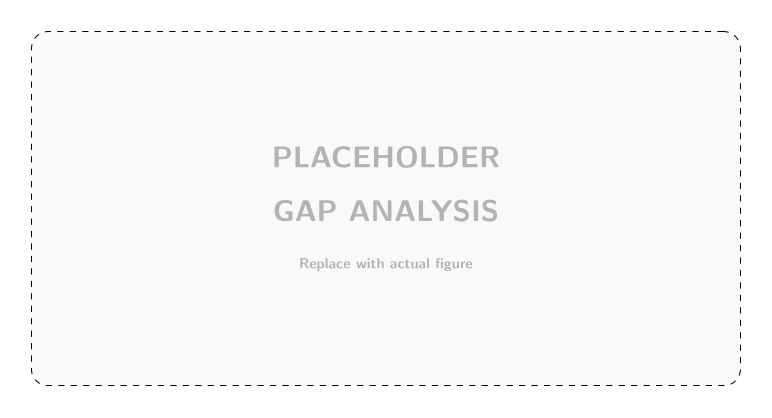
\includegraphics[width=0.85\textwidth]{Images/fig_gap_analysis.png}
\caption{Gap analysis showing unaddressed areas in existing e-voting literature that our system targets.}
\label{fig:gap-analysis}
\end{figure}

Our literature review reveals the following critical gaps:

\begin{enumerate}
    \item \textbf{Trusted Setup Elimination}: Most ZK voting systems (MACI, Semaphore) rely on Groth16, requiring a multi-party computation ceremony. No production voting system has deployed with a setup-free proof system like UltraHonk.
    
    \item \textbf{Gasless ZK Voting}: All existing blockchain voting systems either charge gas fees (excluding economically disadvantaged voters) or use centralized relayers. No system embeds the EVM in a sovereign chain with authority-sponsored execution.
    
    \item \textbf{Multi-Division National Architecture}: Academic prototypes model single-election contracts. Real national elections span hundreds of administrative divisions requiring on-chain aggregation, cross-division Sybil prevention, and delegated administration.
    
    \item \textbf{Mobile Hardware Security for Voting}: Voatz used biometrics but transmitted data to servers. No ZK voting system leverages device hardware keystores for voter secret storage with biometric gates and on-device proof generation.
    
    \item \textbf{Three-Factor Voter Authentication}: Existing systems use either wallet-only (weak) or centralized authentication. No system combines OTP, biometric, and hardware-backed cryptographic identity in a decentralized voting context.
    
    \item \textbf{Vote-Binding in ZK Proofs}: Standard Semaphore signals do not bind the signal content into the proof. This allows front-running attacks where a relayer observes the proof and substitutes a different vote. Our circuit binds the candidate index into the proof statement.
    
    \item \textbf{Administrative Hierarchy Modeling}: No prior work models the full government administrative hierarchy (Election Commission $\to$ District $\to$ Division $\to$ GN Division $\to$ Voter) with on-chain role delegation and access control.
\end{enumerate}

\section{Summary}

This literature review has surveyed the landscape from foundational cryptographic primitives through four generations of electronic voting systems. The key insight is that while individual building blocks exist---ZK proofs, blockchain consensus, mobile authentication, Merkle membership---no prior system integrates them into a cohesive, production-oriented architecture addressing real-world administrative requirements.

Our system (detailed in Chapters~\ref{ch:architecture}--\ref{ch:applications}) addresses each identified gap by combining UltraHonk proving (no trusted setup), a custom gasless blockchain (no economic barriers), multi-division factory contracts (administrative fidelity), and hardware-backed mobile authentication (three-factor security). The following chapter presents the system architecture that synthesizes these components into a unified design.

\chapter{System Architecture and Design}\label{ch:architecture}

This chapter presents the complete system architecture of our privacy-preserving electronic voting system. We establish the design principles that guide all architectural decisions, describe the layered system structure, formally define the threat model, and detail the cryptographic protocols that enable simultaneous voter authentication and ballot privacy.

\section{Design Principles}

Five core principles govern every architectural and implementation decision in our system:

\begin{enumerate}[label=\textbf{P\arabic*}]
    \item \textbf{Zero-Knowledge Privacy}: No entity---including system operators, blockchain validators, or observers---can determine how a specific voter cast their ballot. The system achieves cryptographic unlinkability between voter identity and ballot content.
    
    \item \textbf{Trustless Verification}: All election results are independently verifiable from public on-chain data. No trusted third party (coordinator, mix-net server, or election authority) is required for correctness. Any observer can reconstruct the Merkle tree, re-verify all proofs, and recompute the tally.
    
    \item \textbf{Economic Inclusivity}: Voting must be free for all citizens regardless of economic status. The system eliminates gas fees through a sovereign blockchain with authority-sponsored execution, ensuring that financial barriers never prevent democratic participation.
    
    \item \textbf{Administrative Fidelity}: The system models the real Sri Lankan administrative hierarchy---Election Commission, 22 districts, 160 polling divisions, 14,000+ GN divisions---with on-chain role delegation. This is not a toy prototype; it reflects actual governance structures.
    
    \item \textbf{Defense in Depth}: Security does not rely on any single mechanism. Five independent layers of fraud prevention ensure that compromising one layer does not compromise the election. Each layer addresses a distinct attack vector.
\end{enumerate}

\section{System Architecture Overview}

The system follows a four-layer architecture, each with clear responsibilities and well-defined interfaces:

\begin{figure}[H]
\centering
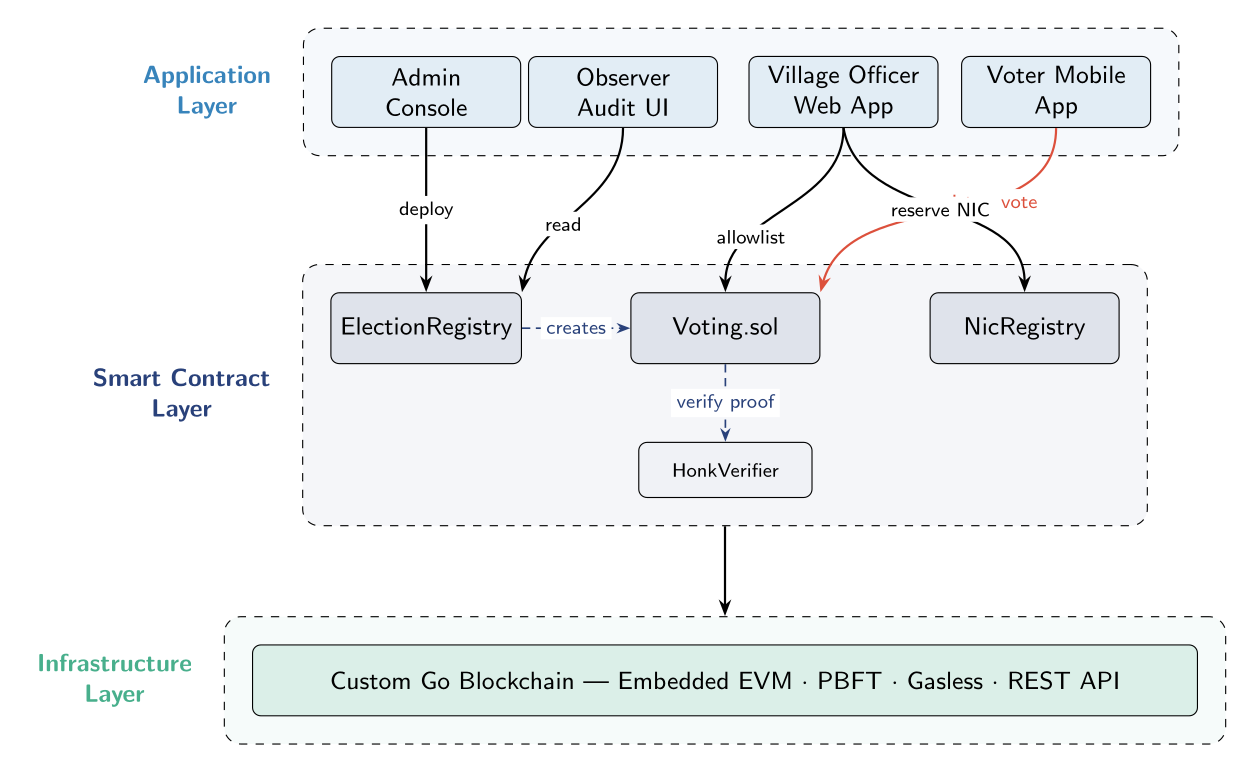
\includegraphics[width=0.85\textwidth]{Images/fig_system_architecture.png}
\caption{Four-layer system architecture showing the application layer, smart contract layer, blockchain infrastructure, and cryptographic foundation.}
\label{fig:system-architecture}
\end{figure}

\subsection{Layer 1: Application Layer}

The application layer provides user-facing interfaces for all system roles:

\begin{table}[H]
\centering
\caption{Application layer components and their target users.}
\label{tab:app-layer}
\begin{tabular}{|l|l|l|l|}
\hline
\textbf{Component} & \textbf{Technology} & \textbf{Users} & \textbf{Functions} \\
\hline
Mobile Voter App & React Native (Expo 54) & Citizens & Identity, Register, Vote, Verify \\
\hline
Admin Console & Next.js (Scaffold-ETH 2) & Election Authority & Division mgmt, Phase control \\
\hline
GN Portal & Next.js & Village Officers & Voter enrollment, NIC check \\
\hline
Results Dashboard & Next.js & Public/Observers & Live tallies, Division breakdown \\
\hline
Audit Interface & Next.js & Auditors & Proof verification, Tree rebuild \\
\hline
\end{tabular}
\end{table}

\subsection{Layer 2: Smart Contract Layer}

Four Solidity contracts implement the election logic:

\begin{table}[H]
\centering
\caption{Smart contract layer with deployment dependencies.}
\label{tab:contract-layer}
\begin{tabular}{|l|l|p{6cm}|}
\hline
\textbf{Contract} & \textbf{Depends On} & \textbf{Responsibility} \\
\hline
\texttt{HonkVerifier.sol} & None & ZK proof verification (auto-generated) \\
\hline
\texttt{Voting.sol} & HonkVerifier & Per-division election state machine \\
\hline
\texttt{ElectionRegistry.sol} & HonkVerifier, Voting & Division factory + national aggregation \\
\hline
\texttt{NicRegistry.sol} & None & Cross-division Sybil prevention \\
\hline
\end{tabular}
\end{table}

\begin{figure}[H]
\centering
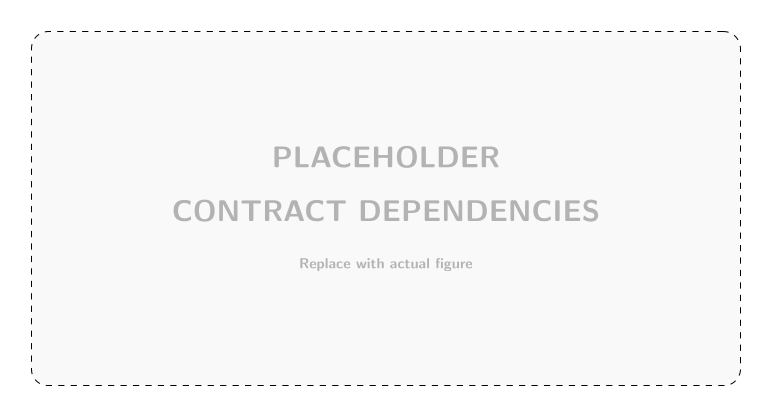
\includegraphics[width=0.85\textwidth]{Images/fig_contract_dependencies.png}
\caption{Contract dependency graph showing the deployment order and interaction patterns between the four smart contracts.}
\label{fig:contract-deps}
\end{figure}

\subsection{Layer 3: Blockchain Infrastructure}

A custom Go blockchain provides the execution environment:
\begin{itemize}
    \item Embedded go-ethereum EVM for Solidity execution
    \item PBFT consensus among election commission nodes
    \item BoltDB persistence for block storage
    \item REST API for application interaction
    \item Gasless execution model (no transaction fees)
    \item mTLS P2P communication between nodes
\end{itemize}

\subsection{Layer 4: Cryptographic Foundation}

The cryptographic layer provides the mathematical guarantees:
\begin{itemize}
    \item BN254 elliptic curve (scalar field $\mathbb{F}_r$, 254-bit security)
    \item Poseidon hash function (algebraically native to $\mathbb{F}_r$)
    \item UltraHonk proof system (no trusted setup, keccak transcript)
    \item LeanIMT incremental Merkle tree ($O(\log n)$ updates and proofs)
\end{itemize}

\section{Threat Model and Adversary Capabilities}

\subsection{Adversary Classes}

We consider three classes of adversaries with increasing capabilities:

\begin{definition}[External Adversary ($\mathcal{A}_{\text{ext}}$)]
An adversary who can observe all public blockchain data, intercept network traffic, and attempt to vote fraudulently. Cannot access voter devices or compromise system infrastructure.
\end{definition}

\begin{definition}[Infrastructure Adversary ($\mathcal{A}_{\text{infra}}$)]
An adversary who controls up to $f < n/3$ blockchain validator nodes, can observe all API traffic, and may attempt to manipulate the election state. Cannot access voter private keys.
\end{definition}

\begin{definition}[Coercing Adversary ($\mathcal{A}_{\text{coerce}}$)]
An adversary who can observe a voter during the voting process and demand proof of how they voted. May offer bribes or threaten consequences.
\end{definition}

\subsection{Trust Assumptions}

Our system makes the following minimal trust assumptions:
\begin{enumerate}
    \item The voter's device hardware is not compromised (TEE/Secure Enclave intact)
    \item At least $2n/3 + 1$ validator nodes are honest (PBFT threshold)
    \item The BN254 discrete logarithm assumption holds
    \item The Poseidon hash function is collision-resistant
    \item The voter performs the voting action in a private environment
\end{enumerate}

\subsection{Attack Surface Analysis}

\begin{table}[H]
\centering
\caption{Attack surface analysis with corresponding defenses.}
\label{tab:attack-surface}
\begin{tabular}{|p{3cm}|p{4cm}|p{5cm}|}
\hline
\textbf{Attack Vector} & \textbf{Adversary Capability} & \textbf{Defense Mechanism} \\
\hline
Double voting & Submit two votes for same election & Nullifier hash uniqueness (on-chain) \\
\hline
Voter impersonation & Obtain voter's commitment & Hardware keystore + biometric gate \\
\hline
Vote buying/selling & Voter proves how they voted & Burner wallet (unlinkable sender) \\
\hline
Ballot stuffing & Add unauthorized votes & ZK proof of Merkle membership \\
\hline
Vote modification & Change ballot after casting & Vote bound into ZK proof \\
\hline
Sybil attack & Register in multiple divisions & NicRegistry hashed-NIC check \\
\hline
Front-running & Observe proof, change vote & Vote-binding in circuit \\
\hline
Replay attack & Resubmit valid proof & Nullifier consumed on-chain \\
\hline
State rollback & Revert blockchain state & PBFT finality (no reorgs) \\
\hline
Admin abuse & Authority manipulates results & Public verifiability + E2E audit \\
\hline
\end{tabular}
\end{table}

\section{Security Properties}

\subsection{Formal Security Theorem}

\begin{theorem}[Voter--Ballot Unlinkability]
\label{thm:unlinkability}
Under the BN254 discrete logarithm assumption and the collision resistance of Poseidon, for any probabilistic polynomial-time adversary $\mathcal{A}$ with access to the complete blockchain state:
\begin{equation}
\Pr\left[\mathcal{A}(\text{chain}, \text{proofs}, \text{nullifiers}) \to (\text{Voter}_i, \text{Ballot}_j)\right] \leq \frac{1}{|\mathcal{V}|} + \text{negl}(\lambda)
\end{equation}
where $|\mathcal{V}|$ is the number of registered voters and $\lambda$ is the security parameter.
\end{theorem}

\begin{proof}[Proof Sketch]
The proof proceeds by reduction to the zero-knowledge property of UltraHonk:
\begin{enumerate}
    \item The ZK proof reveals no information about the prover's identity (zero-knowledge).
    \item The Merkle path is hidden (private input), preventing leaf identification.
    \item The nullifier hash is a one-way function of the secret nullifier.
    \item The vote is submitted from a fresh burner wallet with no prior transaction history.
    \item Therefore, the adversary's view is computationally indistinguishable regardless of which voter cast which ballot.
\end{enumerate}
\end{proof}

\subsection{Double-Vote Prevention}

\begin{property}[Uniqueness]
Each registered voter can cast exactly one valid vote per election:
\begin{equation}
\forall v \in \mathcal{V}: |\{b \in \text{Ballots} : \text{nullifier}(b) = \Poseidon_1(r_v)\}| \leq 1
\end{equation}
\end{property}

This is enforced by the on-chain nullifier set: \texttt{s\_nullifierHashes[electionId][hash] = true}. Once a nullifier hash is consumed, any subsequent proof using the same nullifier is rejected.

\subsection{Eligibility Soundness}

\begin{property}[Eligibility]
Only voters whose commitment is in the Merkle tree can generate a valid proof:
\begin{equation}
\text{Honk.Verify}(\pi, x) = \text{true} \implies \exists \text{ leaf } l \in \text{Tree}(root) : l = \Poseidon_2(r, s)
\end{equation}
\end{property}

This follows from the soundness of the UltraHonk proof system---no polynomial-time adversary can forge a proof of Merkle membership for a commitment not in the tree.

\section{Election Phase State Machine}

The election lifecycle is modeled as a deterministic state machine with four phases:

\begin{figure}[H]
\centering
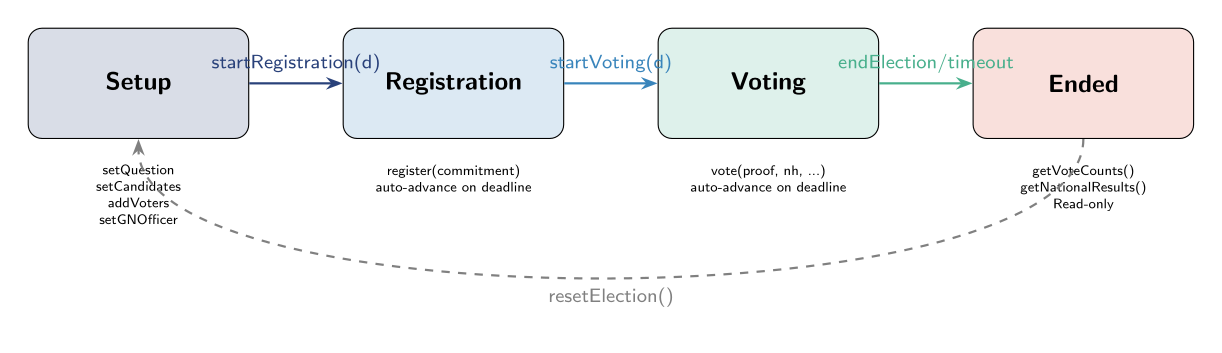
\includegraphics[width=0.85\textwidth]{Images/fig_phases.png}
\caption{Election phase state machine showing transitions, conditions, and automatic deadline-based advancement.}
\label{fig:phases}
\end{figure}

\subsection{Phase Definitions}

\begin{enumerate}
    \item \textbf{Setup Phase}: Administrator configures the election (question, candidates, voter allowlist, GN officer assignment). No time pressure; manual transition.
    
    \item \textbf{Registration Phase}: Allowlisted voters register their cryptographic commitments to the Merkle tree. Deadline-bounded; auto-advances to Voting when \texttt{registrationEndTime} passes.
    
    \item \textbf{Voting Phase}: Registered voters generate ZK proofs and cast anonymous ballots. Deadline-bounded; auto-advances to Ended when \texttt{votingEndTime} passes.
    
    \item \textbf{Ended Phase}: Election is concluded. Results are final and publicly readable. No further state changes permitted.
\end{enumerate}

\subsection{Transition Rules}

\begin{table}[H]
\centering
\caption{Phase transition rules with authorization and conditions.}
\label{tab:transitions}
\begin{tabular}{|l|l|l|p{5cm}|}
\hline
\textbf{Transition} & \textbf{Trigger} & \textbf{Auth} & \textbf{Conditions} \\
\hline
Setup $\to$ Registration & \texttt{startRegistration(d)} & Owner & Duration $> 0$, candidates set \\
\hline
Registration $\to$ Voting & \texttt{startVoting(d)} & Owner & Duration $> 0$, or auto after deadline \\
\hline
Voting $\to$ Ended & \texttt{endElection()} & Owner & Or auto after deadline \\
\hline
Any $\to$ Setup & \texttt{resetElection()} & Owner & Bumps electionId \\
\hline
\end{tabular}
\end{table}

The \texttt{\_maybeAdvancePhase()} modifier automatically checks deadlines on every state-mutating call, ensuring that phase transitions occur even without explicit admin action.

\section{Cryptographic Protocol Design}

\subsection{Commitment Scheme}

During registration, each voter generates a cryptographic commitment that binds their identity to the election without revealing it:

\begin{equation}
\text{commitment} = \Poseidon_2(\text{nullifier}, \text{secret})
\end{equation}

where:
\begin{itemize}
    \item $\text{nullifier} \xleftarrow{\$} \mathbb{F}_r$: random field element, stored in hardware keystore
    \item $\text{secret} \xleftarrow{\$} \mathbb{F}_r$: random field element, stored in hardware keystore
    \item The commitment is a deterministic function of both secrets
\end{itemize}

The commitment serves as the voter's ``ticket'' to the election---it is inserted as a leaf in the Merkle tree during registration.

\subsection{Nullifier Mechanism}

The nullifier provides double-vote prevention while maintaining anonymity:

\begin{equation}
\text{nullifier\_hash} = \Poseidon_1(\text{nullifier})
\end{equation}

\textbf{Key properties}:
\begin{itemize}
    \item Deterministic: same nullifier always produces same hash (prevents double-voting)
    \item One-way: hash cannot be inverted to recover the nullifier (preserves privacy)
    \item Unique per voter: different voters have different nullifiers (distinguishable rejections)
\end{itemize}

\subsection{Merkle Membership Proof}

The voter proves their commitment is in the tree by providing the authentication path:

\begin{equation}
\text{verify\_path}(\text{commitment}, \text{siblings}[0..d-1], \text{index\_bits}[0..d-1]) \stackrel{?}{=} \text{root}
\end{equation}

The path traversal uses little-endian bit decomposition of the leaf index:
\begin{align}
h_0 &= \text{commitment} \\
h_{i+1} &= \begin{cases}
\Poseidon_2(h_i, \text{siblings}[i]) & \text{if } \text{index\_bits}[i] = 0 \\
\Poseidon_2(\text{siblings}[i], h_i) & \text{if } \text{index\_bits}[i] = 1
\end{cases}
\end{align}

The final computed hash $h_d$ must equal the published Merkle root.

\subsection{Complete Protocol Flow}

\begin{algorithm}[H]
\caption{Complete Voting Protocol}
\label{alg:protocol}
\begin{algorithmic}[1]
\STATE \textbf{Registration Phase:}
\STATE Voter generates $(\text{nullifier}, \text{secret}) \xleftarrow{\$} \mathbb{F}_r^2$
\STATE Voter computes $\text{commitment} = \Poseidon_2(\text{nullifier}, \text{secret})$
\STATE Voter submits $\text{register}(\text{commitment})$ to division contract
\STATE Contract inserts commitment into LeanIMT tree
\STATE
\STATE \textbf{Voting Phase:}
\STATE Voter retrieves Merkle path from chain state
\STATE Voter constructs witness $w = (\text{nullifier}, \text{secret}, \text{index}, \text{siblings})$
\STATE Voter constructs public inputs $x = (\Poseidon_1(\text{nullifier}), \text{root}, \text{vote}, \text{depth})$
\STATE Voter generates proof: $\pi \leftarrow \text{UltraHonk.Prove}(x, w)$
\STATE Voter creates burner wallet (fresh keypair)
\STATE Voter funds burner via faucet/paymaster
\STATE Voter submits $\text{vote}(\pi, \text{nullifier\_hash}, \text{root}, \text{vote}, \text{depth})$ from burner
\STATE Contract verifies: $\text{HonkVerifier.verify}(\pi, [x_1, x_2, x_3, x_4])$
\STATE Contract checks: nullifier\_hash not in used set
\STATE Contract increments vote count, records nullifier
\end{algorithmic}
\end{algorithm}

\section{Multi-Division Architecture}

\subsection{Sri Lanka's Electoral Structure}

Sri Lanka's electoral system comprises 22 electoral districts containing 160 polling divisions. Our system models this hierarchy on-chain:

\begin{figure}[H]
\centering
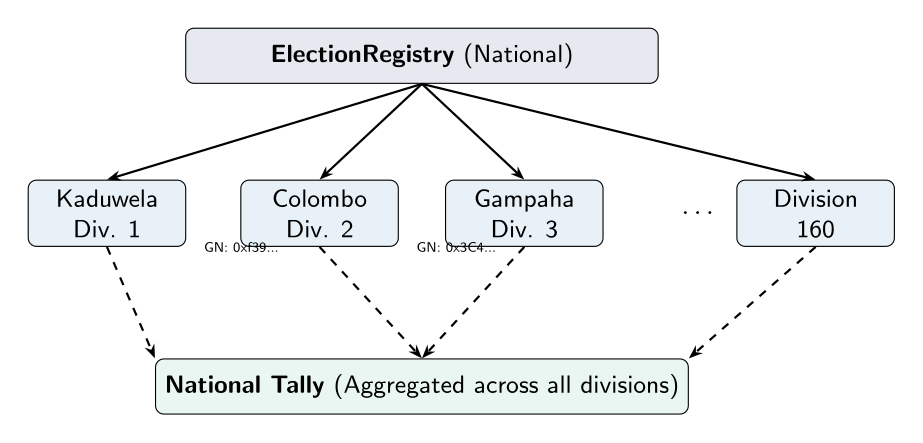
\includegraphics[width=0.85\textwidth]{Images/fig_divisions.png}
\caption{Multi-division architecture: ElectionRegistry deploys 160 independent Voting contracts with national aggregation.}
\label{fig:divisions}
\end{figure}

\subsection{Factory Pattern Design}

The \texttt{ElectionRegistry} contract implements the factory pattern:

\begin{lstlisting}[language=Java, caption={ElectionRegistry factory pattern (simplified).}]
function createDivision(string name) external onlyOwner
    returns (uint256 divisionId, address votingContract)
{
    Voting newVoting = new Voting(i_verifier, msg.sender);
    divisions.push(Division({
        name: name,
        votingContract: address(newVoting),
        gnOfficer: address(0),
        active: true
    }));
    divisionId = divisions.length - 1;
    votingContract = address(newVoting);
}
\end{lstlisting}

\textbf{Design decisions}:
\begin{itemize}
    \item Each division gets an independent \texttt{Voting.sol} instance (isolation)
    \item All share a single \texttt{HonkVerifier} (gas efficiency---deploy once, verify many)
    \item GN officers are assigned per-division (delegated administration)
    \item National aggregation is read-only (no cross-division write dependencies)
\end{itemize}

\subsection{National Result Aggregation}

The registry provides national-level views by summing across all active divisions:

\begin{equation}
\text{NationalVotes}[c] = \sum_{d \in \text{ActiveDivisions}} \text{Division}_d.\text{voteCounts}[c]
\label{eq:national-agg}
\end{equation}

This computation is performed on-chain as a view function (no gas cost), enabling any observer to independently verify the national tally.

\section{Five-Layer Fraud Prevention}

Our system implements defense in depth through five independent fraud prevention layers:

\begin{table}[H]
\centering
\caption{Five-layer fraud prevention architecture.}
\label{tab:fraud-layers}
\begin{tabular}{|c|l|p{4cm}|p{4cm}|}
\hline
\textbf{Layer} & \textbf{Name} & \textbf{Mechanism} & \textbf{Prevents} \\
\hline
1 & Identity Gate & Hardware keystore + biometric & Device-level impersonation \\
\hline
2 & Eligibility Proof & ZK Merkle membership & Unauthorized ballot casting \\
\hline
3 & Uniqueness Enforcement & On-chain nullifier set & Double voting \\
\hline
4 & National De-duplication & NicRegistry (hashed NIC) & Cross-division Sybil \\
\hline
5 & Cryptographic Binding & Vote in proof statement & Front-running, modification \\
\hline
\end{tabular}
\end{table}

\subsection{Layer 1: Identity Gate}

Before any election-related action, the mobile app requires biometric authentication:
\begin{itemize}
    \item Voter's private key stored in \texttt{expo-secure-store} with \texttt{requireAuthentication: true}
    \item Device's Trusted Execution Environment (TEE) or Secure Enclave protects key material
    \item Even with physical device access, keys cannot be extracted without biometric enrollment
\end{itemize}

\subsection{Layer 2: ZK Eligibility Proof}

The zero-knowledge proof demonstrates that the voter's commitment exists in the Merkle tree without revealing which commitment is theirs. A voter who was never registered (no leaf in tree) cannot produce a valid proof.

\subsection{Layer 3: Nullifier Uniqueness}

Each voter's nullifier produces a unique, deterministic hash. The contract maintains a mapping:
\begin{lstlisting}[language=Java, caption={Nullifier uniqueness enforcement.}]
mapping(uint256 electionId => mapping(bytes32 => bool)) s_nullifierHashes;

// In vote():
if (s_nullifierHashes[s_electionId][_nullifierHash])
    revert NullifierHashAlreadyUsed(_nullifierHash);
s_nullifierHashes[s_electionId][_nullifierHash] = true;
\end{lstlisting}

\subsection{Layer 4: NIC Registry}

The \texttt{NicRegistry} stores hashed National Identity Card numbers:
\begin{equation}
\text{nicHash} = \Poseidon(\text{NIC\_number}, \text{SERVER\_PEPPER})
\end{equation}

This prevents a voter from registering in multiple divisions using the same NIC. The server pepper ensures that the NIC hash cannot be computed without the election authority's secret, preventing brute-force enumeration.

\subsection{Layer 5: Vote Binding}

The candidate index is a public input to the ZK circuit:
\begin{lstlisting}[language=Java, caption={Vote binding in the Noir circuit.}]
// Circuit constrains: vote is bound into the proof
vote_bits: [u1; 8] = vote.to_le_bits();
// The proof is only valid for this specific candidate index
\end{lstlisting}

An adversary who intercepts the proof cannot substitute a different vote---the proof is cryptographically bound to the candidate index.

\section{Voting.sol State Machine Design}

\begin{figure}[H]
\centering
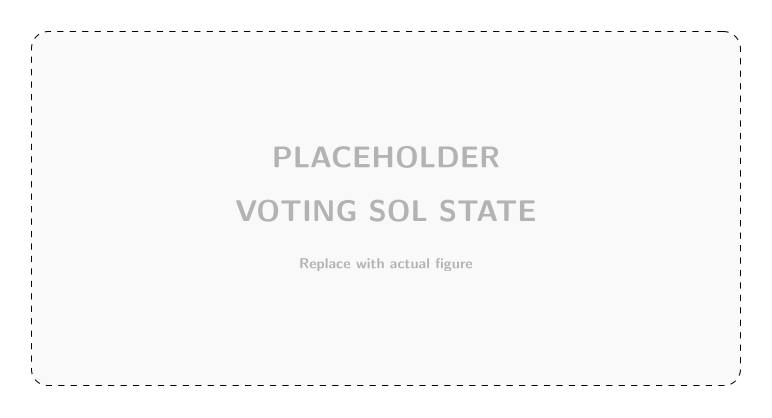
\includegraphics[width=0.85\textwidth]{Images/fig_voting_sol_state.png}
\caption{Detailed state diagram of Voting.sol showing all state variables, transitions, and per-election isolation through electionId keying.}
\label{fig:voting-state}
\end{figure}

\subsection{Per-Election Isolation}

A critical design choice is keying all mutable state by \texttt{electionId}:

\begin{lstlisting}[language=Java, caption={Election-keyed state isolation.}]
// All per-election state is isolated
mapping(uint256 => mapping(address => bool)) s_voters;
mapping(uint256 => mapping(address => bool)) s_hasRegistered;
mapping(uint256 => mapping(uint256 => bool)) s_commitments;
mapping(uint256 => mapping(bytes32 => bool)) s_nullifierHashes;
mapping(uint256 => mapping(uint256 => uint256)) s_voteCounts;
mapping(uint256 => IncrementalTreeData) s_trees;
\end{lstlisting}

When \texttt{resetElection()} is called, the \texttt{electionId} increments. All previous state remains intact (for audit) but is no longer accessible to current-election operations. This enables contract reuse across multiple election cycles without redeployment.

\section{Data Flow Architecture}

The complete data flow from voter action to on-chain state change follows this path:

\begin{enumerate}
    \item \textbf{User Action}: Voter interacts with mobile app
    \item \textbf{Local Cryptography}: Secrets retrieved from keystore, commitment/proof generated
    \item \textbf{Network Transport}: REST API call to custom blockchain node
    \item \textbf{API Handler}: Go HTTP handler validates format, applies rate limits
    \item \textbf{EVM Execution}: Embedded go-ethereum EVM executes Solidity bytecode
    \item \textbf{State Transition}: Contract logic validates and updates state
    \item \textbf{Block Commit}: PBFT consensus finalizes the state change
    \item \textbf{Persistence}: BoltDB stores the committed block
    \item \textbf{Event Emission}: Blockchain events propagate to listening clients
\end{enumerate}

\section{Summary}

This chapter has established the architectural foundation of our privacy-preserving voting system. The four-layer design provides clear separation of concerns while the five-layer fraud prevention ensures defense in depth. The formal security theorem (Theorem~\ref{thm:unlinkability}) provides mathematical assurance of voter--ballot unlinkability. The multi-division factory pattern faithfully models Sri Lanka's 160-division electoral structure. Chapter~\ref{ch:methodology} next describes the development methodology and the iterative journey from initial prototypes to the final architecture presented here.

\chapter{Methodology: Development Journey}\label{ch:methodology}

This chapter narrates the complete development journey of our system---from initial technology evaluation through four iterations of the ZK circuit, three generations of contract architecture, custom blockchain development, and mobile app challenges. Unlike a sanitized methodology section, we present the \textit{actual} path: what we tried, what failed, why it failed, and how each failure informed the next iteration.

\section{Technology Selection Process}

\subsection{ZK Circuit Language: Circom to Noir}

\subsubsection{Initial Attempt: Circom}

Our first implementation attempt used Circom~\cite{belles2022circom}, the most established ZK circuit DSL. We implemented a basic Merkle membership proof in Circom with the following structure:

\begin{lstlisting}[language=Java, caption={Initial Circom circuit attempt (abandoned).}]
template VoteMembership(depth) {
    signal input nullifier;
    signal input secret;
    signal input siblings[depth];
    signal input pathIndices[depth];
    signal output nullifierHash;
    signal output root;
    
    component hasher = Poseidon(2);
    hasher.inputs[0] <== nullifier;
    hasher.inputs[1] <== secret;
    // ... Merkle path verification
}
\end{lstlisting}

\textbf{Problems encountered with Circom}:
\begin{enumerate}
    \item \textbf{R1CS constraint model}: Circom compiles to Rank-1 Constraint Systems, which are less expressive than Plonkish arithmetization. Custom gates (needed for efficient Poseidon) require awkward workarounds.
    \item \textbf{Trusted setup requirement}: Circom targets Groth16, requiring a per-circuit trusted setup ceremony via \texttt{snarkjs powers of tau}. For a university project, coordinating a multi-party ceremony was impractical.
    \item \textbf{JavaScript-centric toolchain}: The \texttt{snarkjs} library generates proofs in Node.js. On React Native's Hermes engine, BigInt operations were unsupported, requiring polyfills that increased proof time from 15s to 90s.
    \item \textbf{Template verbosity}: Circom requires explicit signal wiring for every operation, making the circuit logic spread across 200+ lines for our relatively simple proof.
\end{enumerate}

\subsubsection{Migration to Noir}

Noir~\cite{aztec2024noir}, developed by Aztec Labs, offered a compelling alternative:
\begin{itemize}
    \item \textbf{Rust-like syntax}: High-level, readable code that compiles to ACIR (Abstract Circuit Intermediate Representation)
    \item \textbf{UltraHonk backend}: No trusted setup; the keccak transcript eliminates ceremony coordination
    \item \textbf{Barretenberg (bb.js)}: WASM-ready prover that runs in WebView contexts
    \item \textbf{Built-in Poseidon}: Native stdlib support for Poseidon over BN254
    \item \textbf{Concise expression}: Our entire circuit fits in $\sim$30 lines of Noir
\end{itemize}

The migration from Circom to Noir reduced our circuit from 210 lines to 28 lines while simultaneously eliminating the trusted setup requirement. This was the first major architectural decision that shaped the entire system.

\begin{figure}[H]
\centering
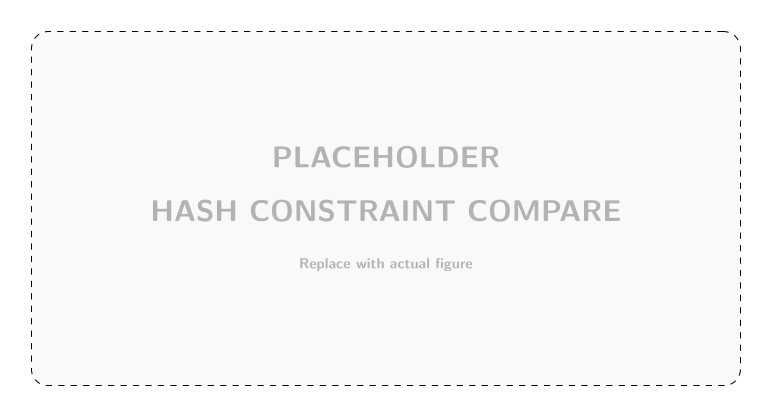
\includegraphics[width=0.85\textwidth]{Images/fig_hash_constraint_compare.png}
\caption{Constraint count comparison between Circom+Groth16 and Noir+UltraHonk for equivalent circuit logic.}
\label{fig:hash-constraint}
\end{figure}

\subsection{Hash Function: SHA-256 to Poseidon}

\subsubsection{SHA-256 Attempt}

Our earliest prototype used SHA-256 for all hashing (commitments, Merkle nodes, nullifiers). This choice seemed natural---SHA-256 is the most widely deployed hash function and has extensive security analysis.

\textbf{What we observed}: The Circom SHA-256 circuit required approximately 25,000 constraints per hash invocation. With a depth-16 Merkle tree requiring 17 hash computations (1 commitment + 16 path nodes), the total circuit size exceeded 425,000 constraints. Proof generation on a mobile device was estimated at 3--5 minutes---completely unacceptable for user experience.

\subsubsection{Why SHA-256 Fails in Arithmetic Circuits}

SHA-256 operates on 32-bit words with bitwise operations (XOR, AND, rotation). In an arithmetic circuit over $\mathbb{F}_p$, each bit operation requires:
\begin{itemize}
    \item Range checks to ensure values are boolean
    \item Decomposition/recomposition between field elements and bit arrays
    \item Simulated bitwise operations using arithmetic ($a \oplus b = a + b - 2ab$ in $\mathbb{F}_p$)
\end{itemize}

\subsubsection{Poseidon Solution}

Poseidon's algebraic design uses only field multiplications and additions---operations that are \textit{native} to the arithmetic circuit. The S-box $x \mapsto x^5$ is a single multiplication gate in UltraHonk.

\textbf{Result}: Circuit size dropped from 425,000 to approximately 5,100 constraints. Proof generation time decreased from minutes to 15--30 seconds in WebView WASM.

\subsection{Blockchain Platform: Ethereum to L2 to Custom}

\begin{figure}[H]
\centering
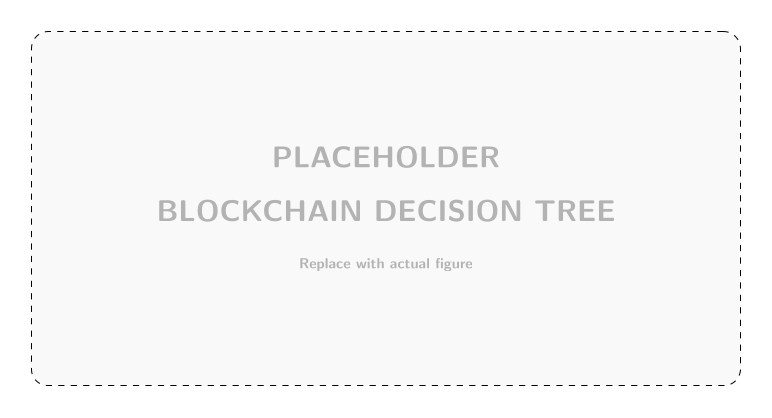
\includegraphics[width=0.85\textwidth]{Images/fig_blockchain_decision_tree.png}
\caption{Decision tree showing our evaluation of blockchain platforms and why we built a custom chain.}
\label{fig:blockchain-decision}
\end{figure}

\subsubsection{Phase 1: Ethereum Mainnet}

Initial development targeted Ethereum mainnet using Hardhat for local testing. We successfully deployed and tested all contracts on the Hardhat local node.

\textbf{Blocking issue}: Gas costs. A single \texttt{vote()} transaction costs approximately 350,000 gas ($\sim$\$15 at 30 gwei). For 16 million voters, this represents an impossible economic barrier. Even with gas sponsorship, the total cost would exceed \$240 million.

\subsubsection{Phase 2: Layer 2 Evaluation}

We evaluated several L2 solutions:

\begin{table}[H]
\centering
\caption{L2 platform evaluation for voting workload.}
\label{tab:l2-eval}
\begin{tabular}{|l|l|l|l|}
\hline
\textbf{Platform} & \textbf{Vote Cost} & \textbf{Finality} & \textbf{Blocking Issue} \\
\hline
Arbitrum & \$0.05--0.20 & 7 days (L1) & Still costs money \\
\hline
Optimism & \$0.05--0.15 & 7 days (L1) & Still costs money \\
\hline
Base & \$0.01--0.05 & 7 days (L1) & Still costs money \\
\hline
Polygon PoS & \$0.001 & 2 hours & Reorg risk \\
\hline
\end{tabular}
\end{table}

\textbf{Fundamental insight}: Any public chain---L1 or L2---charges fees. Even \$0.001 per vote $\times$ 16M voters = \$16,000. More critically, it creates a dependency on cryptocurrency markets and wallet funding that is inappropriate for a national election.

\subsubsection{Phase 3: Custom Go Blockchain}

The decision to build a custom blockchain was driven by three non-negotiable requirements:
\begin{enumerate}
    \item \textbf{Zero cost}: Voting must be economically free
    \item \textbf{Deterministic finality}: No reorgs or probabilistic confirmation
    \item \textbf{Sovereignty}: No dependency on external networks or token economics
\end{enumerate}

The custom blockchain embeds go-ethereum's EVM package, executing the \textit{same compiled Solidity bytecode} as our Hardhat tests. This architectural choice means our 54 unit tests validate the exact code running in production.

\subsection{Mobile Framework: Flutter to React Native}

\begin{figure}[H]
\centering
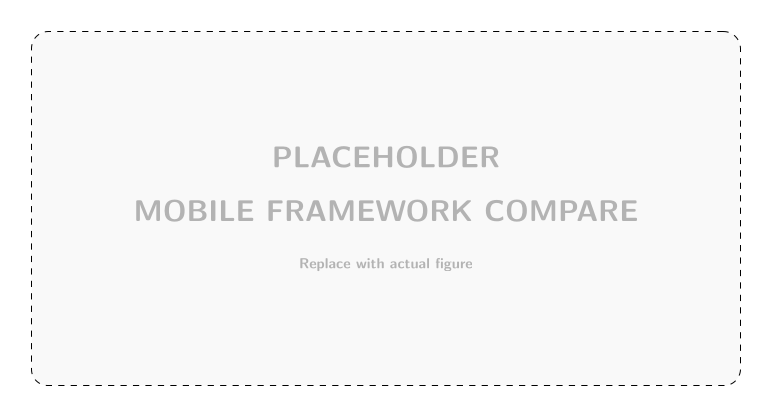
\includegraphics[width=0.85\textwidth]{Images/fig_mobile_framework_compare.png}
\caption{Mobile framework evaluation against our ZK voting requirements.}
\label{fig:mobile-framework}
\end{figure}

\subsubsection{Flutter Evaluation}

Flutter (Dart) was initially considered for its cross-platform capabilities and native performance. However:
\begin{itemize}
    \item No mature EVM library for Dart (web3dart is unmaintained)
    \item No equivalent of \texttt{expo-secure-store} with biometric gating
    \item WebView integration is less mature (no \texttt{react-native-webview} equivalent for WASM proving)
    \item Smaller ecosystem for blockchain-related packages
\end{itemize}

\subsubsection{React Native (Expo) Selection}

React Native with Expo SDK 54 was selected for:
\begin{itemize}
    \item \textbf{viem}: Production-grade EVM interaction library with TypeScript types
    \item \textbf{expo-secure-store}: Hardware-backed keychain with biometric authentication
    \item \textbf{expo-local-authentication}: Unified biometric API (fingerprint + face)
    \item \textbf{WebView}: Mature react-native-webview for hosting WASM bb.js prover
    \item \textbf{poseidon-lite}: JavaScript Poseidon implementation for commitment generation
\end{itemize}

\section{ZK Circuit Evolution}

Our circuit went through four major iterations, each addressing failures discovered in the previous version.

\subsection{Iteration 1: Basic Membership (Failed)}

\begin{figure}[H]
\centering
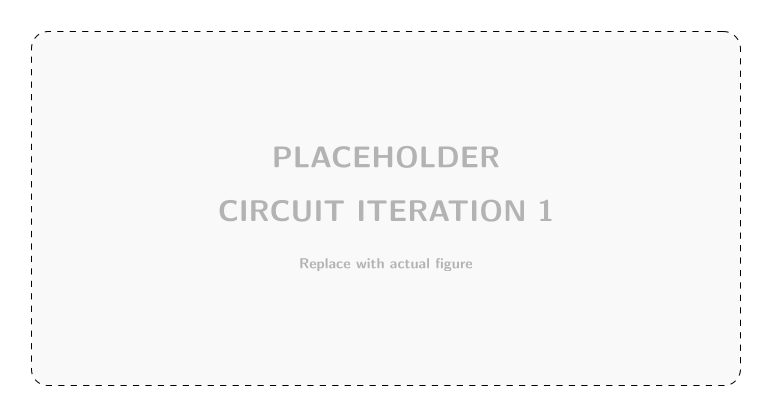
\includegraphics[width=0.85\textwidth]{Images/fig_circuit_iteration_1.png}
\caption{Circuit iteration 1: basic Merkle membership without vote binding or nullifier constraints.}
\label{fig:circuit-v1}
\end{figure}

The first iteration proved only Merkle membership:
\begin{lstlisting}[language=Java, caption={Circuit v1: basic membership (incomplete).}]
fn main(
    root: pub Field,
    nullifier: Field, secret: Field,
    index: Field, siblings: [Field; 16],
) {
    let commitment = poseidon2([nullifier, secret]);
    let computed_root = merkle_root(commitment, siblings, index);
    assert(computed_root == root);
}
\end{lstlisting}

\textbf{Failure}: The vote was not part of the proof. An attacker observing the mempool could extract the valid proof and submit it with a different vote value. The vote was passed as a separate contract parameter with no cryptographic binding.

\subsection{Iteration 2: Vote Binding Added (Partially Failed)}

We added the vote as a public input, binding it into the proof:
\begin{lstlisting}[language=Java, caption={Circuit v2: added vote binding.}]
fn main(
    nullifier_hash: pub Field,
    root: pub Field,
    vote: pub Field,  // NEW: bound into proof
    // ... same private inputs
)
\end{lstlisting}

\textbf{Partial failure}: The nullifier hash was computed \textit{off-chain} and passed as public input without being constrained to match the private nullifier. A malicious voter could submit someone else's nullifier hash while proving with their own secrets---the circuit would not catch the mismatch.

\subsection{Iteration 3: Nullifier Constraint (Subtle Bug)}

We added the nullifier hash verification:
\begin{lstlisting}[language=Java, caption={Circuit v3: nullifier constraint added.}]
assert(poseidon1([nullifier]) == nullifier_hash);
\end{lstlisting}

\textbf{Subtle bug}: The Merkle path used big-endian bit decomposition for the index, but the on-chain LeanIMT tree used little-endian ordering. Proofs verified locally but failed on-chain because the computed root differed when traversing left/right children in reversed order.

\textbf{Diagnosis}: This took 3 days to identify. We generated proofs that passed the Noir prover but failed HonkVerifier on-chain. The error was ``InvalidRoot''---the proof was technically valid, but proved membership in a differently-ordered tree.

\subsection{Iteration 4: Final Correct Circuit}

\begin{figure}[H]
\centering
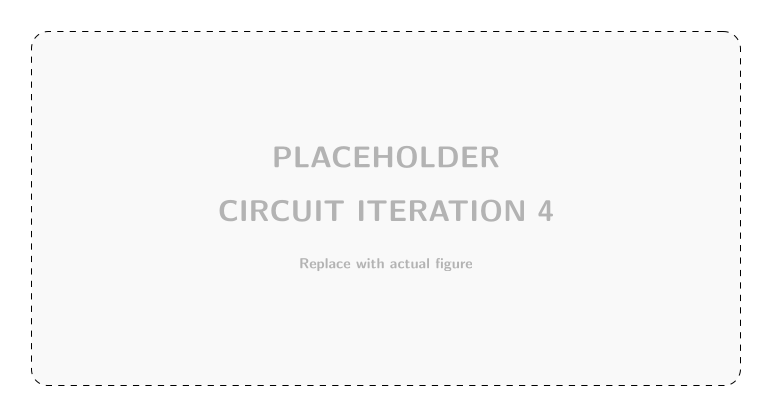
\includegraphics[width=0.85\textwidth]{Images/fig_circuit_iteration_4.png}
\caption{Circuit iteration 4 (final): all constraints correct, matching on-chain tree ordering.}
\label{fig:circuit-v4}
\end{figure}

The final circuit uses \texttt{index.to\_le\_bits()} (little-endian), matching the LeanIMT on-chain implementation:

\begin{lstlisting}[language=Java, caption={Final Noir circuit (v4) with all constraints.}]
fn main(
    nullifier_hash: pub Field,
    root: pub Field,
    vote: pub Field,
    depth: pub u32,
    nullifier: Field,
    secret: Field,
    index: Field,
    siblings: [Field; 16],
) {
    // 1. Nullifier binding
    assert(poseidon1([nullifier]) == nullifier_hash);
    
    // 2. Commitment derivation
    let commitment = poseidon2([nullifier, secret]);
    
    // 3. Merkle membership (little-endian index bits)
    let index_bits = index.to_le_bits();
    let computed = binary_merkle_root(
        hash_2, commitment, depth, index_bits, siblings
    );
    assert(computed == root);
    
    // 4. Vote range check (8-bit)
    let _vote_bits: [u1; 8] = vote.to_le_bits();
}
\end{lstlisting}

\section{Smart Contract Architecture Evolution}

\subsection{Version 1: Monolithic Contract}

\begin{figure}[H]
\centering
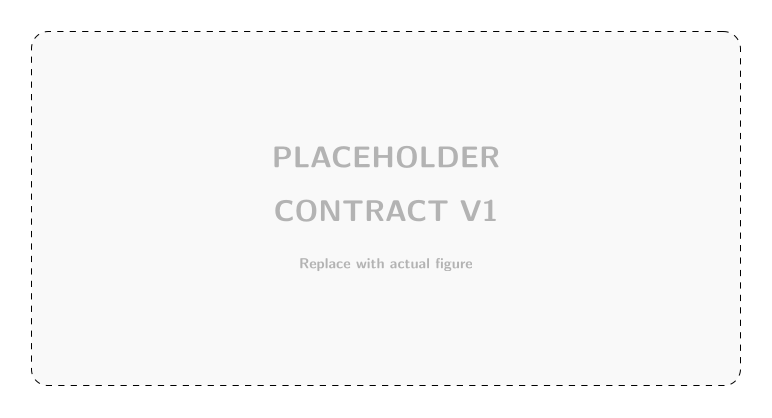
\includegraphics[width=0.85\textwidth]{Images/fig_contract_v1.png}
\caption{Contract v1: single monolithic contract handling all divisions and all logic.}
\label{fig:contract-v1}
\end{figure}

The first contract version was a single \texttt{Voting.sol} that managed all 160 divisions internally:
\begin{lstlisting}[language=Java, caption={Contract v1: monolithic (abandoned).}]
mapping(uint256 divisionId => MerkleTree) trees;
mapping(uint256 divisionId => Phase) phases;
mapping(uint256 divisionId => mapping(uint256 => uint256)) voteCounts;
\end{lstlisting}

\textbf{Problems}:
\begin{itemize}
    \item Gas cost scaled with division count for any lookup
    \item Single point of failure: a bug in one division's logic affected all
    \item Access control complexity: every function needed a divisionId parameter
    \item Deployment bytecode exceeded Ethereum's 24KB contract size limit
\end{itemize}

\subsection{Version 2: Manual Multi-Contract}

We manually deployed separate Voting contracts and tracked them off-chain. This worked but required:
\begin{itemize}
    \item Manual coordination of 160 deployments
    \item Off-chain registry of contract addresses
    \item No on-chain national aggregation
    \item Manual GN officer assignment (error-prone)
\end{itemize}

\subsection{Version 3: Factory Pattern (Final)}

\begin{figure}[H]
\centering
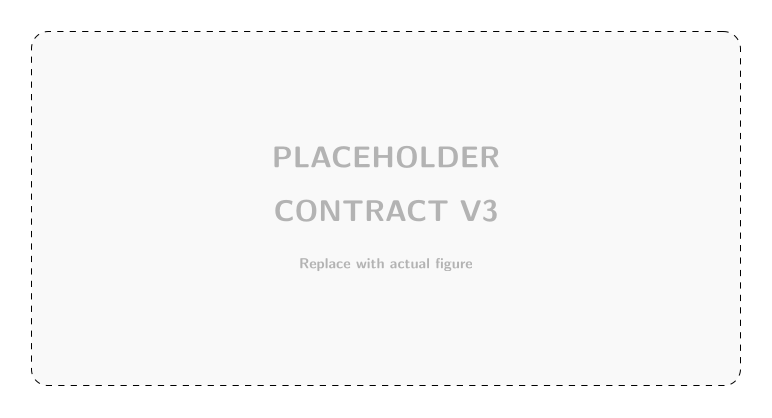
\includegraphics[width=0.85\textwidth]{Images/fig_contract_v3.png}
\caption{Contract v3 (final): ElectionRegistry factory pattern with per-division Voting instances.}
\label{fig:contract-v3}
\end{figure}

The final architecture uses the factory pattern with three key contracts:
\begin{enumerate}
    \item \texttt{ElectionRegistry}: Factory that deploys and manages Voting instances
    \item \texttt{Voting}: Per-division election state machine (isolated)
    \item \texttt{NicRegistry}: Global NIC de-duplication across all divisions
\end{enumerate}

This provides isolation (a bug in one division cannot affect others), on-chain aggregation (national results computed by summing across divisions), and administrative delegation (GN officers per division).

\section{Custom Blockchain Development Challenges}

\subsection{EVM Embedding}

\textbf{Challenge}: Running Solidity contracts inside a custom blockchain required embedding the go-ethereum EVM. This is not a documented use case---go-ethereum is designed as a standalone node, not an embeddable library.

\textbf{What we tried}: Initially, we attempted to use go-ethereum's \texttt{ethclient} package to connect to an external node. This worked but defeated the purpose of a sovereign chain.

\textbf{Final approach}: We imported go-ethereum's \texttt{core/vm} package directly, creating a custom \texttt{StateDB} implementation backed by BoltDB:

\begin{lstlisting}[language=Java, caption={EVM embedding in Go (simplified).}]
// Create EVM context
blockCtx := vm.BlockContext{
    BlockNumber: new(big.Int).SetUint64(blockNum),
    Time:        uint64(time.Now().Unix()),
    GasLimit:    16_000_000,
}

// Execute contract call
evm := vm.NewEVM(blockCtx, txCtx, stateDB, chainConfig, vmConfig)
ret, _, err := evm.Call(caller, contractAddr, calldata, gasLimit, value)
\end{lstlisting}

\textbf{Key insight}: The EVM itself is stateless---it reads/writes through the StateDB interface. By implementing this interface ourselves, we could use any backing store (BoltDB in our case) while executing the exact same bytecode as Ethereum mainnet.

\subsection{Gasless Execution Model}

\textbf{Challenge}: Standard EVM execution charges gas, deducting from the sender's balance. In our gasless model, voters have zero balance.

\textbf{Solution}: We set the gas limit to 16M for all transactions and never deduct gas costs. The EVM still \textit{meters} gas (for DoS protection and infinite loop prevention) but we do not subtract from any account balance. The authority (election commission) implicitly sponsors all execution.

\subsection{StateDB Implementation}

The most complex challenge was implementing go-ethereum's \texttt{StateDB} interface, which includes:
\begin{itemize}
    \item Account balance/nonce management
    \item Contract code storage/retrieval
    \item Storage slot read/write (per-contract key-value store)
    \item Log (event) emission
    \item Snapshot/revert for atomic transactions
    \item Suicide (selfdestruct) handling
\end{itemize}

Our implementation uses BoltDB buckets for persistence, with an in-memory dirty cache for pending state changes that are flushed on block commit.

\subsection{BN254 Precompile for Proof Verification}

\textbf{Challenge}: The HonkVerifier contract calls the BN254 pairing precompile at address \texttt{0x08}. Go-ethereum includes these precompiles, but they must be explicitly registered in the chain configuration.

\textbf{What failed initially}: We used a minimal chain config without precompile registration. HonkVerifier calls succeeded in Hardhat (which registers all precompiles by default) but reverted with ``execution reverted'' on our custom chain.

\textbf{Fix}: Register all Istanbul-era precompiles in our custom EVM configuration, including ecRecover (0x01), SHA-256 (0x02), RIPEMD-160 (0x03), identity (0x04), modexp (0x05), ecAdd (0x06), ecMul (0x07), and ecPairing (0x08).

\section{Mobile Development Challenges}

\subsection{Hermes Engine BigInt Crisis}

\begin{figure}[H]
\centering
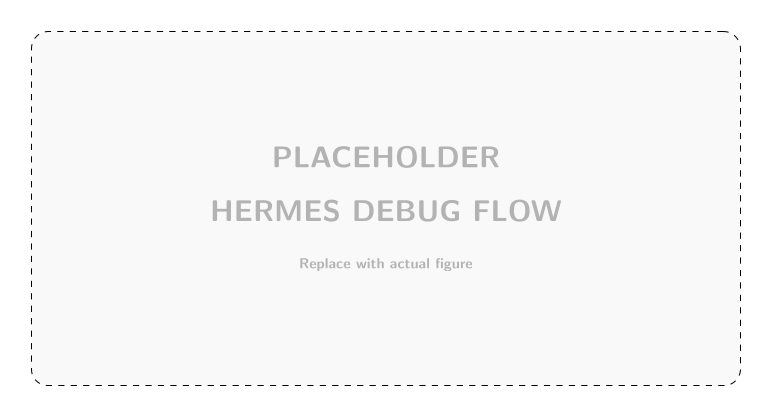
\includegraphics[width=0.85\textwidth]{Images/fig_hermes_debug_flow.png}
\caption{Debugging flow for the Hermes BigInt incompatibility: from cryptic error to WebView solution.}
\label{fig:hermes-debug}
\end{figure}

\textbf{The problem}: React Native uses the Hermes JavaScript engine (not V8). Hermes does not support native BigInt. Our entire cryptographic pipeline (Poseidon, field arithmetic, proof generation) relies on BigInt for 254-bit field element arithmetic.

\textbf{What we observed}: Importing \texttt{poseidon-lite} crashed immediately with ``BigInt is not defined''. The \texttt{viem} library (which uses BigInt for transaction encoding) also failed.

\textbf{Attempted solutions}:
\begin{enumerate}
    \item \textbf{BigInt polyfill (JSBI)}: Added JSBI polyfill, but poseidon-lite uses BigInt literals (\texttt{21888...n}) which cannot be polyfilled at the syntax level.
    \item \textbf{babel-plugin-transform-bigint}: Transforms BigInt syntax to JSBI calls. Partially worked for our code but broke library internals that used \texttt{BigInt()} constructor.
    \item \textbf{ethers.js v5}: Used its bundled BigNumber polyfill. Worked for basic operations but could not be used with poseidon-lite.
\end{enumerate}

\textbf{Final solution}: A hybrid architecture:
\begin{itemize}
    \item \textbf{poseidon-lite}: Used in a React Native WebView (which runs V8/JavaScriptCore with native BigInt support)
    \item \textbf{viem}: Used with legacy transaction signing (manually constructing RLP-encoded transactions without BigInt-dependent auto-estimation)
    \item \textbf{ZK proof generation}: Entirely in WebView via bb.js WASM
\end{itemize}

\subsection{WebView ZK Proving Architecture}

\begin{figure}[H]
\centering
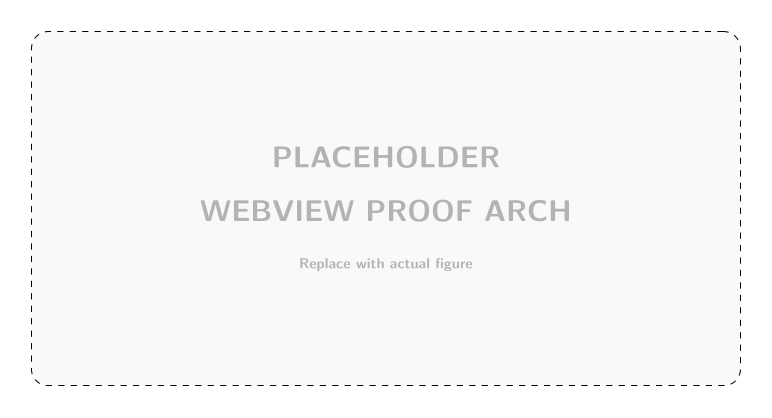
\includegraphics[width=0.85\textwidth]{Images/fig_webview_proof_arch.png}
\caption{WebView-based proof generation architecture: React Native passes witness data to an embedded WebView running bb.js WASM.}
\label{fig:webview-arch}
\end{figure}

The WebView proving pipeline works as follows:
\begin{enumerate}
    \item React Native constructs the circuit witness (using field arithmetic in WebView)
    \item Witness is serialized and passed to the proving WebView via \texttt{postMessage}
    \item WebView loads bb.js WASM module and compiled ACIR circuit
    \item bb.js generates the UltraHonk proof (15--30 seconds)
    \item Proof bytes are returned to React Native via \texttt{onMessage} callback
    \item React Native constructs the transaction calldata from proof bytes
\end{enumerate}

\subsection{Biometric Authentication Integration}

\textbf{Challenge}: \texttt{expo-local-authentication} provides biometric prompts, but \texttt{expo-secure-store} has its own authentication gate. Coordinating these two systems to provide a seamless single-prompt experience required careful state management.

\textbf{Key decision}: We set \texttt{requireAuthentication: true} on sensitive keystore items (private key, nullifier, secret) but \texttt{false} on non-sensitive items (address, division selection, voted flags). This means accessing secrets triggers a single OS-level biometric prompt, while reading public state does not interrupt the user.

\subsection{Legacy Transaction Signing}

\textbf{Challenge}: viem's \texttt{sendTransaction} uses EIP-1559 gas estimation internally, which calls BigInt operations. On Hermes, this crashes.

\textbf{Solution}: We manually construct legacy (pre-EIP-1559) transactions:
\begin{lstlisting}[language=Java, caption={Manual legacy transaction construction for Hermes compatibility.}]
// Build raw transaction manually (no BigInt auto-estimation)
const tx = {
  to: contractAddress,
  data: encodeFunctionData(...),
  gasLimit: "0x" + (500000).toString(16),
  gasPrice: "0x0",  // gasless chain
  nonce: "0x" + nonce.toString(16),
  chainId: 31337,
};
const signed = await signTransaction(privateKey, tx);
const hash = await sendRawTransaction(signed);
\end{lstlisting}

\section{Integration Challenges}

\subsection{Poseidon Field Mismatch}

\textbf{The bug}: When testing end-to-end (mobile $\to$ blockchain $\to$ on-chain verification), proofs generated on mobile were rejected on-chain with ``InvalidProof''.

\textbf{Root cause}: The \texttt{poseidon-lite} npm package uses a slightly different round constant derivation than the Noir stdlib's Poseidon. Both are ``Poseidon over BN254'' but produce different outputs for the same input due to different MDS matrices.

\textbf{Detection}: We generated test vectors---hashing the same value in both environments and comparing outputs. The mismatch was immediately visible.

\textbf{Fix}: We ensured both the mobile app and the Noir circuit use the exact same Poseidon parameterization (the one from circomlibjs/poseidon-lite). The Noir stdlib's \texttt{std::hash::poseidon} matched this parameterization, but we needed to verify by generating matching test vectors.

\subsection{Bit Ordering: The Three-Day Bug}

\textbf{Symptom}: Proofs for tree index 0 and 1 verified correctly, but index 2 and above failed on-chain.

\textbf{Investigation}: For index 0 (binary: 000...0) and index 1 (binary: 000...1), the bit ordering (big-endian vs. little-endian) produces the same path traversal. Starting at index 2 (binary: 10 LE vs. 01 BE), the difference manifests.

\textbf{Resolution}: Changed circuit to use \texttt{to\_le\_bits()} matching the LeanIMT library's convention of treating the least-significant bit as the first tree level.

\subsection{Public Input Ordering}

\textbf{The problem}: The HonkVerifier expects public inputs in a specific order: \texttt{[nullifier\_hash, root, vote, depth]}. The order is determined by the Noir compiler's output, which follows the declaration order in the circuit function signature.

\textbf{What happened}: We initially passed inputs as \texttt{[root, nullifier\_hash, vote, depth]} (alphabetical order in our contract code). The verifier silently verified against wrong values and returned false.

\textbf{Lesson}: Public input ordering must exactly match the circuit's function signature parameter order. We added a comment in the contract code documenting this requirement.

\section{Development Methodology}

\subsection{Iterative Bottom-Up Approach}

We followed an iterative bottom-up methodology rather than a waterfall approach:

\begin{enumerate}
    \item \textbf{Cryptographic Core First}: ZK circuit correctness is the foundation. We invested 6 weeks perfecting the circuit before writing any application code.
    \item \textbf{Contract Testing}: 54 unit tests validate all contract behavior before integration. Tests are run after every change.
    \item \textbf{Vertical Slices}: Each feature was implemented as a complete vertical slice (mobile $\to$ API $\to$ contract $\to$ verification) before moving to the next.
    \item \textbf{Continuous Integration Testing}: End-to-end proof generation and verification tested after each circuit or contract change.
\end{enumerate}

\subsection{Tools and Environment}

\begin{table}[H]
\centering
\caption{Development tools and their roles in our workflow.}
\label{tab:dev-tools}
\begin{tabular}{|l|l|l|}
\hline
\textbf{Tool} & \textbf{Version} & \textbf{Purpose} \\
\hline
Nargo & 1.0.0-beta.3 & Noir circuit compilation and testing \\
\hline
Hardhat & 2.22 & Solidity compilation, testing, deployment \\
\hline
Go & 1.21 & Custom blockchain implementation \\
\hline
Expo & SDK 54 & React Native mobile app development \\
\hline
Next.js & 14.x & Web application framework \\
\hline
Barretenberg (bb) & 0.82.x & Proof generation and verification \\
\hline
Yarn & 4.13.0 & Monorepo package management \\
\hline
\end{tabular}
\end{table}

\section{Summary of Key Decisions}

\begin{table}[H]
\centering
\caption{Summary of technology decisions with rationale.}
\label{tab:decisions-summary}
\resizebox{\textwidth}{!}{%
\begin{tabular}{|l|l|l|p{5cm}|}
\hline
\textbf{Decision} & \textbf{Rejected} & \textbf{Selected} & \textbf{Key Rationale} \\
\hline
Circuit DSL & Circom & Noir & No trusted setup, readable syntax, WASM prover \\
\hline
Hash function & SHA-256 & Poseidon & 83$\times$ fewer constraints in circuit \\
\hline
Proof system & Groth16 & UltraHonk & No ceremony, faster mobile proving \\
\hline
Blockchain & Ethereum/L2 & Custom Go & Zero gas fees, sovereignty, PBFT finality \\
\hline
Mobile & Flutter & React Native & viem, expo-secure-store, WebView WASM \\
\hline
Contracts & Monolithic & Factory & Isolation, scalability, delegation \\
\hline
Key storage & AsyncStorage & expo-secure-store & Hardware TEE, biometric gate \\
\hline
Signing & EIP-1559 & Legacy tx & Hermes BigInt incompatibility workaround \\
\hline
\end{tabular}%
}
\end{table}

Each decision was arrived at through practical experience with the rejected alternative---not theoretical analysis alone. This empirical approach ensured that our final architecture addresses real, observed problems rather than hypothetical concerns. Chapter~\ref{ch:circuit} details the final ZK circuit implementation that emerged from these four iterations.

\chapter{Zero-Knowledge Circuit Implementation}\label{ch:circuit}

This chapter provides a comprehensive analysis of our ZK circuit implementation in Noir. We detail the circuit's input specification, Poseidon hash internals, Merkle tree membership proof, complete code listing with line-by-line analysis, constraint complexity, the UltraHonk proof system, on-chain verifier parameters, and the formal security properties achieved.

\section{Circuit Requirements}

The circuit must prove the following compound statement in zero knowledge:

\begin{quote}
\textit{``I know a secret nullifier $r$ and secret $s$ such that $\Poseidon_2(r, s)$ is a leaf in the Merkle tree with the given root, and $\Poseidon_1(r)$ equals the given nullifier hash, and I am voting for candidate $v$.''}
\end{quote}

This statement simultaneously achieves:
\begin{itemize}
    \item \textbf{Eligibility}: Only registered voters (with commitment in tree) can prove
    \item \textbf{Privacy}: The prover's identity (which leaf) is hidden
    \item \textbf{Uniqueness}: The nullifier hash deterministically identifies the voter for double-vote prevention
    \item \textbf{Vote binding}: The candidate choice is cryptographically bound into the proof
\end{itemize}

\subsection{Input Specification}

\begin{table}[H]
\centering
\caption{Complete circuit input specification with types, visibility, and purpose.}
\label{tab:circuit-inputs}
\begin{tabular}{|l|l|l|l|p{5cm}|}
\hline
\textbf{Name} & \textbf{Type} & \textbf{Visibility} & \textbf{Source} & \textbf{Purpose} \\
\hline
\texttt{nullifier\_hash} & Field & Public & Derived on-device & Double-vote prevention \\
\hline
\texttt{root} & Field & Public & From chain state & Merkle tree root (current) \\
\hline
\texttt{vote} & Field & Public & User selection & Candidate index \\
\hline
\texttt{depth} & u32 & Public & From chain state & Tree depth for path verification \\
\hline
\texttt{nullifier} & Field & Private & Hardware keystore & Secret nullifier (biometric-gated) \\
\hline
\texttt{secret} & Field & Private & Hardware keystore & Secret commitment seed \\
\hline
\texttt{index} & Field & Private & From chain state & Leaf position in tree \\
\hline
\texttt{siblings} & [Field; 16] & Private & From chain state & Merkle authentication path \\
\hline
\end{tabular}
\end{table}

\begin{figure}[H]
\centering
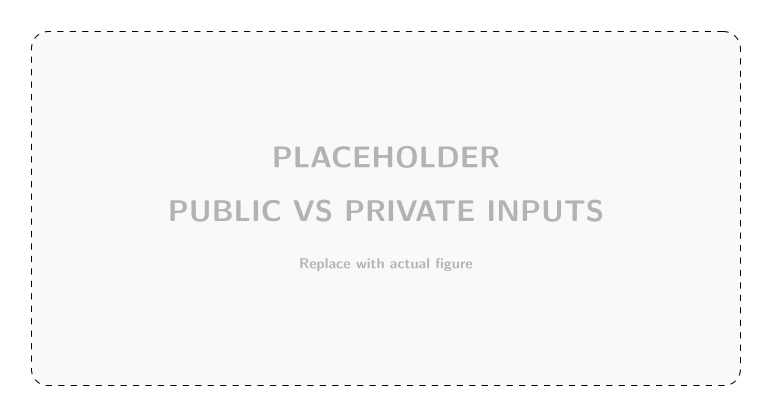
\includegraphics[width=0.85\textwidth]{Images/fig_public_vs_private_inputs.png}
\caption{Public vs. private input separation: public inputs are verified on-chain; private inputs are known only to the prover.}
\label{fig:public-private}
\end{figure}

\section{Poseidon Hash Function Internals}

\subsection{Sponge Construction}

Poseidon uses a sponge construction with state width $t$, rate $r$, and capacity $c = t - r$:

\begin{figure}[H]
\centering
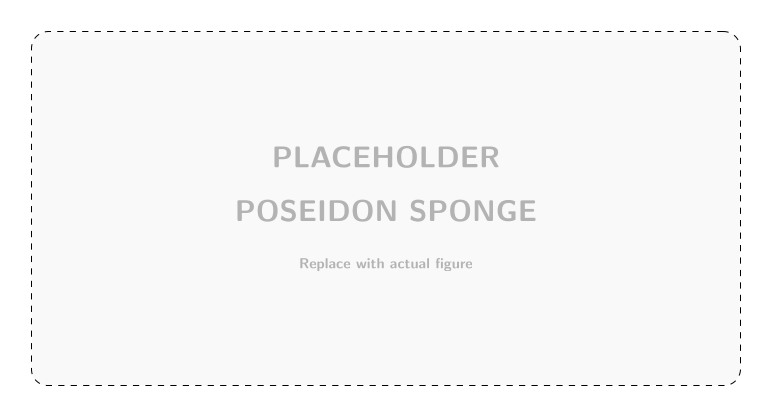
\includegraphics[width=0.85\textwidth]{Images/fig_poseidon_sponge.png}
\caption{Poseidon sponge construction: absorb phase loads inputs into the rate portion; squeeze phase extracts the output hash.}
\label{fig:poseidon-sponge}
\end{figure}

\subsection{Round Function}

Each round of the Poseidon permutation consists of three operations:

\begin{equation}
\text{Round}(S) = \text{MDS} \cdot \text{S-box}(\text{ARK}(S))
\end{equation}

where:
\begin{itemize}
    \item $\text{ARK}(S) = S + C_i$ (Add Round Key: element-wise addition of round constants)
    \item $\text{S-box}(x) = x^5$ (Power map over $\mathbb{F}_r$, chosen for security margin)
    \item $\text{MDS}$ is a Maximum Distance Separable matrix multiplication for diffusion
\end{itemize}

\subsection{Full vs. Partial Rounds}

For security against algebraic attacks while minimizing constraints:
\begin{itemize}
    \item \textbf{Full rounds} ($R_f = 8$): S-box applied to all state elements (diffusion)
    \item \textbf{Partial rounds} ($R_p$): S-box applied to only the first state element (efficiency)
\end{itemize}

For our BN254 instantiation with $t=3$:
\begin{align}
R_f &= 8 \quad \text{(4 before + 4 after partial rounds)} \\
R_p &= 57 \quad \text{(partial rounds)} \\
\text{Total rounds} &= 65
\end{align}

\subsection{Constraint Cost Analysis}

Each full round costs $t$ multiplication gates (one per S-box). Each partial round costs 1 multiplication gate. The MDS multiplication is linear (free in arithmetic circuits). Therefore:

\begin{equation}
\text{Constraints per } \Poseidon_2 \approx R_f \cdot t + R_p = 8 \times 3 + 57 = 81 \text{ multiplication gates}
\end{equation}

In UltraHonk's Plonkish arithmetization, this translates to approximately 300 constraints including the linear operations.

\section{Merkle Tree Membership Proof}

\subsection{Binary Merkle Tree Structure}

\begin{figure}[H]
\centering
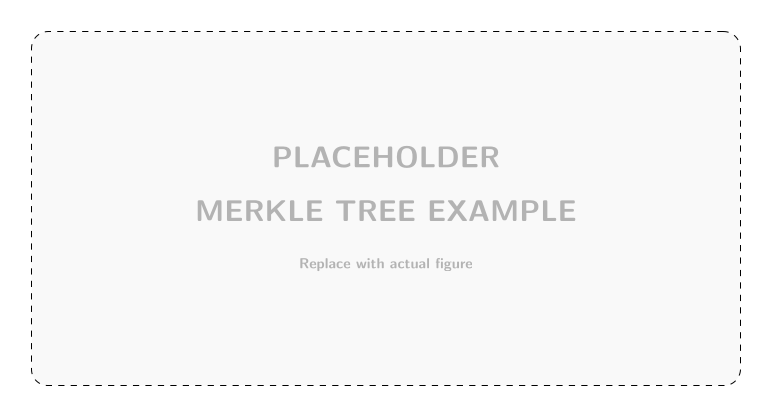
\includegraphics[width=0.85\textwidth]{Images/fig_merkle_tree_example.png}
\caption{Depth-4 Merkle tree example: leaf $l_5$ proves membership by revealing siblings (shaded) along its authentication path.}
\label{fig:merkle-example}
\end{figure}

A binary Merkle tree of depth $d$ stores up to $2^d$ leaves. Each internal node is computed as:
\begin{equation}
\text{node}(i, j) = \Poseidon_2(\text{child\_left}(i, j), \text{child\_right}(i, j))
\end{equation}

\subsection{Authentication Path}

To prove that leaf $l$ is in the tree with root $R$, the prover provides:
\begin{itemize}
    \item The leaf value $l$ (or values that derive it)
    \item The leaf index $i$ (determines left/right placement at each level)
    \item The sibling hash at each level: $\text{siblings}[0], \ldots, \text{siblings}[d-1]$
\end{itemize}

The verifier recomputes the root:
\begin{align}
h_0 &= l \\
h_{k+1} &= \begin{cases}
\Poseidon_2(h_k, \text{siblings}[k]) & \text{if } \text{index\_bits}[k] = 0 \text{ (leaf is left child)} \\
\Poseidon_2(\text{siblings}[k], h_k) & \text{if } \text{index\_bits}[k] = 1 \text{ (leaf is right child)}
\end{cases}
\end{align}

The bit decomposition uses \textbf{little-endian} ordering: bit $k$ of the index determines the direction at tree level $k$ (bottom to top).

\subsection{Variable-Depth Support}

Our tree supports variable depth (up to 16). For a tree with actual depth $d < 16$, the siblings array is padded with zeros for levels $d$ through 15. The circuit uses the \texttt{depth} public input to determine how many levels to traverse.

\section{Complete Noir Circuit Listing}

\begin{lstlisting}[language=Java, caption={Complete Noir ZK voting circuit (main.nr).}, label={lst:circuit}]
use std::hash::poseidon;
use std::hash::poseidon2::Poseidon2;

// Helper: Poseidon hash of single field element
fn poseidon1(input: [Field; 1]) -> Field {
    poseidon::bn254::hash_1(input)
}

// Helper: Poseidon hash of two field elements
fn poseidon2(input: [Field; 2]) -> Field {
    poseidon::bn254::hash_2(input)
}

// Binary Merkle root computation
fn binary_merkle_root<let N: u32>(
    hash_2: fn([Field; 2]) -> Field,
    leaf: Field,
    depth: u32,
    index_bits: [u1; N],
    siblings: [Field; N],
) -> Field {
    let mut current = leaf;
    for i in 0..N {
        if i as u32 < depth {
            let (left, right) = if index_bits[i] == 0 {
                (current, siblings[i])
            } else {
                (siblings[i], current)
            };
            current = hash_2([left, right]);
        }
    }
    current
}

// Main circuit function
fn main(
    nullifier_hash: pub Field,
    root: pub Field,
    vote: pub Field,
    depth: pub u32,
    nullifier: Field,
    secret: Field,
    index: Field,
    siblings: [Field; 16],
) {
    // Constraint 1: Nullifier hash binding
    assert(poseidon1([nullifier]) == nullifier_hash);
    
    // Constraint 2: Commitment derivation
    let commitment = poseidon2([nullifier, secret]);
    
    // Constraint 3: Merkle membership proof
    let index_bits: [u1; 16] = index.to_le_bits();
    let computed_root = binary_merkle_root(
        poseidon2, commitment, depth, index_bits, siblings
    );
    assert(computed_root == root);
    
    // Constraint 4: Vote range check (8-bit)
    let _vote_bits: [u1; 8] = vote.to_le_bits();
}
\end{lstlisting}

\subsection{Line-by-Line Analysis}

\begin{table}[H]
\centering
\caption{Detailed analysis of each circuit constraint.}
\label{tab:constraint-analysis}
\begin{tabular}{|c|p{3cm}|p{4cm}|p{4cm}|}
\hline
\textbf{Line} & \textbf{Operation} & \textbf{Purpose} & \textbf{Security Property} \\
\hline
48 & \texttt{poseidon1([nullifier])} & Compute hash of private nullifier & Binds proof to voter identity \\
\hline
48 & \texttt{== nullifier\_hash} & Assert matches public input & Prevents nullifier substitution \\
\hline
51 & \texttt{poseidon2([null, sec])} & Compute commitment & Links to registered Merkle leaf \\
\hline
54 & \texttt{index.to\_le\_bits()} & Decompose index to bits & Determines path traversal direction \\
\hline
55--57 & \texttt{binary\_merkle\_root} & Compute root from path & Proves set membership \\
\hline
59 & \texttt{== root} & Assert matches chain root & Prevents stale/forged proofs \\
\hline
62 & \texttt{vote.to\_le\_bits()} & 8-bit range check on vote & Prevents overflow attacks \\
\hline
\end{tabular}
\end{table}

\section{Constraint Analysis and Complexity}

\subsection{Constraint Breakdown}

\begin{figure}[H]
\centering
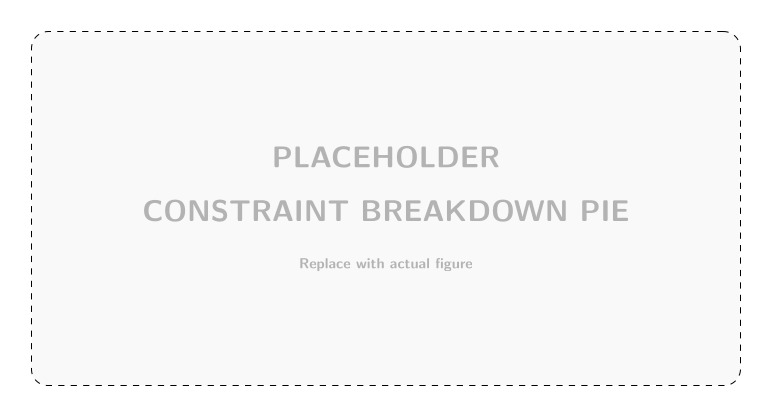
\includegraphics[width=0.85\textwidth]{Images/fig_constraint_breakdown_pie.png}
\caption{Constraint breakdown by operation: Merkle path (16 Poseidon hashes) dominates the circuit size.}
\label{fig:constraint-pie}
\end{figure}

\begin{table}[H]
\centering
\caption{Detailed constraint cost per circuit operation.}
\label{tab:constraint-costs}
\begin{tabular}{|l|r|r|}
\hline
\textbf{Operation} & \textbf{Constraints} & \textbf{Percentage} \\
\hline
Nullifier hash ($\Poseidon_1$) & $\sim$300 & 5.9\% \\
\hline
Commitment ($\Poseidon_2$) & $\sim$300 & 5.9\% \\
\hline
Merkle path (16 $\times$ $\Poseidon_2$) & $\sim$4,800 & 94.1\% \\
\hline
Index bit decomposition & $\sim$16 & 0.3\% \\
\hline
Vote range check & $\sim$8 & 0.2\% \\
\hline
Equality assertions & $\sim$2 & $<$0.1\% \\
\hline
\textbf{Total} & $\sim$5,126 & 100\% \\
\hline
\end{tabular}
\end{table}

\subsection{Asymptotic Complexity}

The circuit complexity scales with tree depth $d$:
\begin{equation}
|\text{Circuit}| = O(d \cdot |\Poseidon_2|) = O(d)
\end{equation}

For our maximum depth of 16, this supports $2^{16} = 65,536$ voters per division. With 160 divisions, the system supports up to $160 \times 65,536 \approx 10.5$ million voters without any circuit modification.

\subsection{Compiled Circuit Size}

After compilation by Nargo to ACIR and then to UltraHonk gates:
\begin{itemize}
    \item \textbf{ACIR opcodes}: $\sim$5,200
    \item \textbf{UltraHonk gates}: $N = 32,768$ ($2^{15}$, next power of 2)
    \item \textbf{LOG\_N}: 15
    \item \textbf{Circuit file size}: $\sim$45 KB (ACIR JSON)
\end{itemize}

\section{UltraHonk Proof System Architecture}

\subsection{Overview}

UltraHonk is a PlonK-variant proof system that eliminates the need for a trusted setup ceremony by using a keccak-based Fiat--Shamir transcript instead of a structured reference string (SRS).

\begin{figure}[H]
\centering
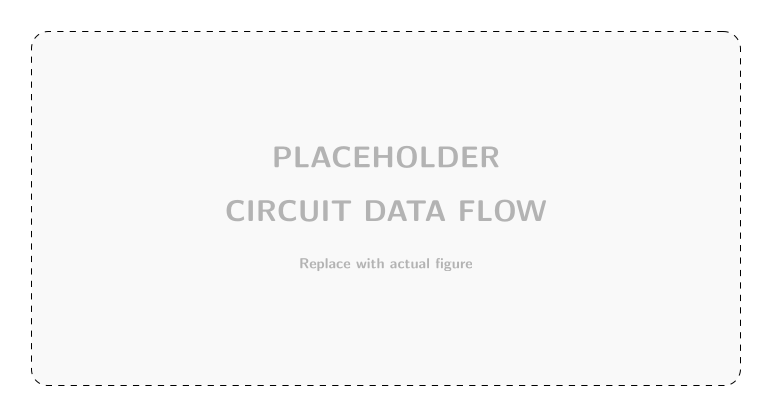
\includegraphics[width=0.85\textwidth]{Images/fig_circuit_data_flow.png}
\caption{UltraHonk proof system data flow: from circuit compilation through ACIR to proof generation and on-chain verification.}
\label{fig:circuit-dataflow}
\end{figure}

\subsection{Arithmetization: Plonkish Constraints}

UltraHonk uses a generalized Plonkish arithmetization supporting:
\begin{itemize}
    \item Standard arithmetic gates: $q_L \cdot a + q_R \cdot b + q_O \cdot c + q_M \cdot (a \cdot b) + q_C = 0$
    \item Custom gates for Poseidon (external and internal rounds)
    \item Lookup tables for range checks
    \item Permutation arguments for wire connections
\end{itemize}

\subsection{Commitment Scheme: KZG on BN254}

Polynomial commitments use the Kate--Zaverucha--Goldberg (KZG) scheme:
\begin{equation}
\text{Commit}(f) = [f(\tau)]_1 = f(\tau) \cdot G_1
\end{equation}

where $\tau$ is the secret evaluation point from the universal SRS. For UltraHonk, the SRS is derived from the Aztec ``ignition'' ceremony (a one-time universal setup supporting circuits up to $2^{28}$ gates).

\subsection{Proof Structure}

An UltraHonk proof consists of:
\begin{enumerate}
    \item Wire polynomial commitments: $[W_1]_1, [W_2]_1, [W_3]_1, [W_4]_1$
    \item Permutation polynomial commitment: $[Z]_1$
    \item Lookup polynomial commitments
    \item Quotient polynomial commitments: $[T_1]_1, [T_2]_1, [T_3]_1, [T_4]_1$
    \item Opening evaluations at challenge point $\zeta$
    \item KZG opening proof: $[W_\zeta]_1, [W_{\zeta\omega}]_1$
\end{enumerate}

Total proof size: approximately 2--4 KB (variable depending on circuit structure).

\section{On-Chain Verifier: HonkVerifier.sol}

\subsection{Auto-Generated Parameters}

The \texttt{HonkVerifier.sol} contract is auto-generated by the Barretenberg compiler from the circuit's verification key:

\begin{lstlisting}[language=Java, caption={HonkVerifier key parameters.}]
uint256 constant N = 32768;           // Circuit size (power of 2)
uint256 constant LOG_N = 15;          // log2(N)
uint256 constant NUMBER_OF_PUBLIC_INPUTS = 4;

// Verification key contains:
// - Selector polynomial commitments (ql, qr, qo, q4, qm, qc, ...)
// - Permutation polynomial commitments (sigma1..4)
// - Identity polynomial commitments (id1..4)
// - Poseidon-specific selectors (qPoseidon2External, qPoseidon2Internal)
\end{lstlisting}

\subsection{Verification Algorithm}

The on-chain verification proceeds in constant time regardless of circuit size:

\begin{algorithm}[H]
\caption{On-Chain Honk Verification (simplified)}
\label{alg:verify}
\begin{algorithmic}[1]
\STATE Parse proof bytes into commitments and evaluations
\STATE Reconstruct Fiat--Shamir challenges from transcript (keccak)
\STATE Compute linearization polynomial evaluation
\STATE Verify KZG opening using BN254 pairing precompile (0x08):
\STATE \quad $e([W_\zeta] + \zeta[W_{\zeta\omega}], [1]_2) \stackrel{?}{=} e([P] + \zeta\omega[W_{\zeta\omega}], [\tau]_2)$
\STATE \textbf{return} pairing check result
\end{algorithmic}
\end{algorithm}

\subsection{Gas Cost}

The verification gas cost is dominated by the BN254 pairing check:
\begin{itemize}
    \item EC additions (precompile 0x06): 150 gas each
    \item EC multiplications (precompile 0x07): 6,000 gas each
    \item Pairing check (precompile 0x08): 45,000 + 34,000 per pair
    \item \textbf{Total verification}: $\sim$280,000 gas
\end{itemize}

\section{Proof Generation Pipeline}

\begin{figure}[H]
\centering
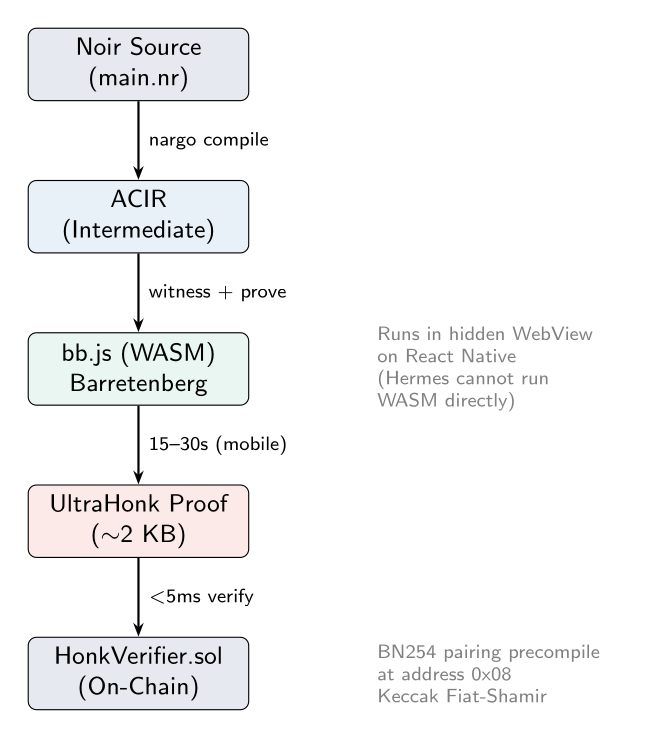
\includegraphics[width=0.85\textwidth]{Images/fig_proof_pipeline.png}
\caption{Complete proof generation pipeline from Noir source code through ACIR compilation to on-chain verification.}
\label{fig:proof-pipeline}
\end{figure}

The end-to-end pipeline consists of five stages:

\begin{enumerate}
    \item \textbf{Circuit Compilation} (build time):
    \begin{itemize}
        \item Nargo compiles \texttt{main.nr} to ACIR (Abstract Circuit Intermediate Representation)
        \item ACIR is a serialized constraint system format
        \item Output: \texttt{circuit.json} ($\sim$45 KB)
    \end{itemize}
    
    \item \textbf{Verification Key Generation} (build time):
    \begin{itemize}
        \item Barretenberg processes ACIR to generate the verification key
        \item Key contains commitments to fixed circuit polynomials
        \item Output: \texttt{HonkVerifier.sol} (auto-generated Solidity contract)
    \end{itemize}
    
    \item \textbf{Witness Computation} (runtime, on device):
    \begin{itemize}
        \item Mobile app constructs the witness from voter secrets and chain state
        \item Witness includes all private inputs satisfying the circuit constraints
    \end{itemize}
    
    \item \textbf{Proof Generation} (runtime, in WebView WASM):
    \begin{itemize}
        \item bb.js WASM module loads ACIR circuit and witness
        \item UltraHonk prover generates the proof (15--30 seconds on mobile)
        \item Output: proof bytes ($\sim$2--4 KB)
    \end{itemize}
    
    \item \textbf{On-Chain Verification} (runtime, EVM):
    \begin{itemize}
        \item Contract calls \texttt{HonkVerifier.verify(proof, publicInputs)}
        \item Verifier uses BN254 precompile for pairing check
        \item Returns boolean: valid or invalid
    \end{itemize}
\end{enumerate}

\section{Security Properties}

\subsection{Computational Soundness}

\begin{theorem}[Soundness]
No probabilistic polynomial-time adversary can produce a valid proof for a false statement (non-member commitment) except with negligible probability:
\begin{equation}
\Pr[\text{Verify}(\pi^*, x) = \text{true} \wedge x \notin L] \leq \text{negl}(\lambda)
\end{equation}
\end{theorem}

This follows from the knowledge soundness of UltraHonk, which is reducible to the algebraic group model (AGM) and the hardness of discrete logarithm on BN254.

\subsection{Zero-Knowledge Property}

\begin{theorem}[Honest-Verifier Zero-Knowledge]
There exists a simulator $S$ that, given only the public inputs $x$, can produce transcripts computationally indistinguishable from real proofs:
\begin{equation}
\{(x, \pi) : \pi \leftarrow P(x, w)\} \approx_c \{(x, \pi^*) : \pi^* \leftarrow S(x)\}
\end{equation}
\end{theorem}

This ensures that the proof reveals nothing about the private witness (nullifier, secret, index, siblings).

\subsection{Double-Vote Prevention}

The nullifier mechanism provides deterministic linkability within a single election:
\begin{equation}
\text{nullifier\_hash} = \Poseidon_1(\text{nullifier}) \quad \text{(deterministic)}
\end{equation}

Two valid proofs from the same voter necessarily produce the same nullifier hash. The contract rejects the second submission, preventing double voting while maintaining anonymity.

\subsection{Front-Running Resistance}

The vote candidate index is a public input bound into the proof:
\begin{equation}
\text{Verify}(\pi, [\text{null\_hash}, \text{root}, v, d]) = \text{true} \implies \text{proof was generated for candidate } v
\end{equation}

An adversary who observes the proof in the mempool cannot extract a valid proof for a different candidate---the proof is cryptographically bound to the specific vote value $v$.

\section{Summary}

This chapter has provided a complete technical analysis of our ZK circuit, from the mathematical foundations of Poseidon and Merkle trees through the Noir implementation to the UltraHonk proof system and on-chain verification. The circuit achieves a constraint count of approximately 5,100 (dominated by 16 Poseidon hashes for the Merkle path), generates proofs in 15--30 seconds on mobile devices, and verifies on-chain in approximately 280,000 gas. The formal security properties (soundness, zero-knowledge, double-vote prevention, and front-running resistance) provide mathematical guarantees suitable for a national-scale election system. Chapter~\ref{ch:contracts} details the smart contracts that consume and enforce these proofs.

\chapter{Smart Contracts and Custom Blockchain}\label{ch:contracts}

This chapter presents the complete implementation of our smart contract layer and custom Go blockchain. We analyze each contract in detail---state variables, events, modifiers, and functions---then describe the custom blockchain architecture including EVM embedding, gasless execution, REST API, PBFT consensus, and BoltDB persistence.

\section{Smart Contract Overview}

Four Solidity contracts compose the election logic, deployed in strict dependency order:

\begin{figure}[H]
\centering
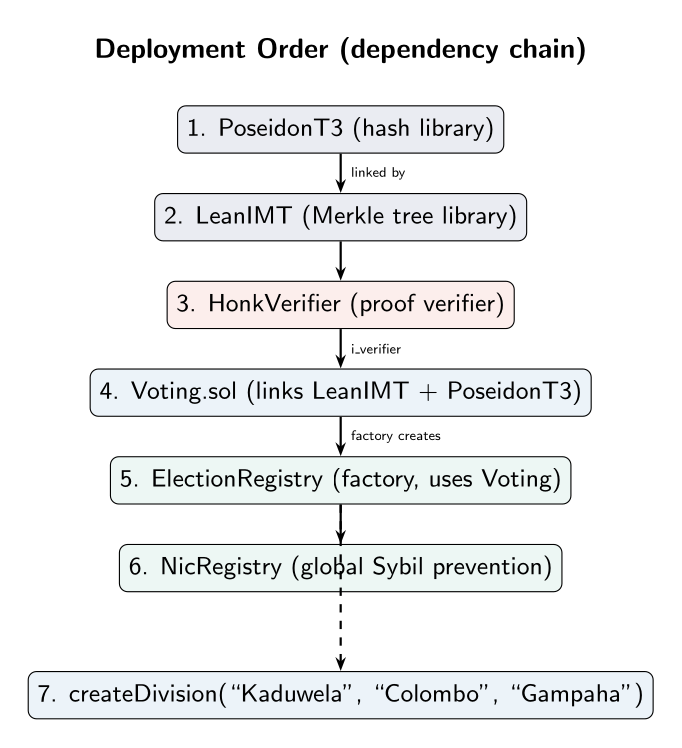
\includegraphics[width=0.85\textwidth]{Images/fig_deploy_order.png}
\caption{Contract deployment order showing dependencies: HonkVerifier must exist before Voting, which must exist before ElectionRegistry can create divisions.}
\label{fig:deploy-order}
\end{figure}

\section{Voting.sol: Per-Division Election State Machine}

\texttt{Voting.sol} is the core contract implementing a complete election lifecycle for a single polling division.

\subsection{State Variables}

\begin{lstlisting}[language=Java, caption={Voting.sol state variable declarations.}]
// Immutables (set at construction)
IHonkVerifier private immutable i_verifier;

// Constants
uint256 public constant MAX_CANDIDATES = 100;

// Administration
address public s_gnOfficer;
string public s_question;
string[] public s_candidates;

// Phase management
uint256 public s_registrationEndTime;
uint256 public s_votingEndTime;
Phase public s_phase;

// Per-election state (keyed by electionId)
uint256 public s_electionId;
mapping(uint256 => mapping(address => bool)) public s_voters;
mapping(uint256 => mapping(address => bool)) public s_hasRegistered;
mapping(uint256 => mapping(uint256 => bool)) public s_commitments;
mapping(uint256 => mapping(bytes32 => bool)) public s_nullifierHashes;
mapping(uint256 => mapping(uint256 => uint256)) public s_voteCounts;
mapping(uint256 => IncrementalTreeData) internal s_trees;
\end{lstlisting}

\subsection{Events}

\begin{lstlisting}[language=Java, caption={Voting.sol event declarations.}]
event VoterAdded(address indexed voter);
event GNOfficerUpdated(address indexed gnOfficer);
event NewLeaf(uint256 index, uint256 value);
event QuestionUpdated(string question);
event CandidatesUpdated(string[] candidates);
event PhaseChanged(Phase indexed phase, uint256 deadline);
event ElectionReset(uint256 indexed electionId);
event VoteCast(
    bytes32 nullifierHash,
    address voter,
    uint256 candidate,
    uint256 timestamp,
    uint256 newCount
);
\end{lstlisting}

\subsection{Custom Errors}

Gas-efficient custom errors replace \texttt{require} strings:

\begin{lstlisting}[language=Java, caption={Custom error declarations for precise revert reasons.}]
error CommitmentAlreadyAdded(uint256 commitment);
error NullifierHashAlreadyUsed(bytes32 nullifierHash);
error InvalidProof();
error NotAllowedToVote();
error EmptyTree();
error InvalidRoot();
error WrongPhase(Phase expected, Phase actual);
error InvalidCandidate(uint256 index);
error InvalidDuration();
error TooManyCandidates(uint256 provided, uint256 max);
error NoCandidates();
\end{lstlisting}

\subsection{Modifiers}

\begin{lstlisting}[language=Java, caption={Phase enforcement and access control modifiers.}]
modifier inPhase(Phase expected) {
    _maybeAdvancePhase();  // Auto-advance if deadline passed
    if (s_phase != expected)
        revert WrongPhase(expected, s_phase);
    _;
}

modifier onlyOwnerOrGN() {
    if (msg.sender != owner() && msg.sender != s_gnOfficer)
        revert OwnableUnauthorizedAccount(msg.sender);
    _;
}
\end{lstlisting}

The \texttt{\_maybeAdvancePhase()} internal function checks block timestamps against stored deadlines and advances the phase accordingly, ensuring consistent behavior regardless of when transactions arrive.

\subsection{Registration Function}

\begin{lstlisting}[language=Java, caption={Voter registration: commitment insertion into Merkle tree.}]
function register(uint256 _commitment) 
    external inPhase(Phase.Registration) 
{
    uint256 eid = s_electionId;
    
    // Check 1: Voter is on the allowlist
    if (!s_voters[eid][msg.sender])
        revert NotAllowedToVote();
    
    // Check 2: Voter hasn't already registered
    if (s_hasRegistered[eid][msg.sender])
        revert NotAllowedToVote();
    
    // Check 3: Commitment is unique
    if (s_commitments[eid][_commitment])
        revert CommitmentAlreadyAdded(_commitment);
    
    // Insert into Merkle tree (LeanIMT)
    uint256 leafIndex = LeanIMT._insert(
        s_trees[eid], _commitment
    );
    
    // Update state
    s_hasRegistered[eid][msg.sender] = true;
    s_commitments[eid][_commitment] = true;
    
    emit NewLeaf(leafIndex, _commitment);
}
\end{lstlisting}

\subsection{Vote Function}

\begin{lstlisting}[language=Java, caption={Anonymous vote casting with ZK proof verification.}]
function vote(
    bytes memory _proof,
    bytes32 _nullifierHash,
    bytes32 _root,
    bytes32 _vote,
    bytes32 _depth
) external inPhase(Phase.Voting) {
    uint256 eid = s_electionId;
    uint256 candidateIdx = uint256(_vote);
    
    // Check 1: Valid candidate index
    if (candidateIdx >= s_candidates.length)
        revert InvalidCandidate(candidateIdx);
    
    // Check 2: Root matches current tree
    if (s_trees[eid]._root() == 0)
        revert EmptyTree();
    if (bytes32(s_trees[eid]._root()) != _root)
        revert InvalidRoot();
    
    // Check 3: Verify ZK proof
    bytes32[] memory publicInputs = new bytes32[](4);
    publicInputs[0] = _nullifierHash;
    publicInputs[1] = _root;
    publicInputs[2] = _vote;
    publicInputs[3] = _depth;
    
    if (!i_verifier.verify(_proof, publicInputs))
        revert InvalidProof();
    
    // Check 4: Nullifier not already used
    if (s_nullifierHashes[eid][_nullifierHash])
        revert NullifierHashAlreadyUsed(_nullifierHash);
    
    // State updates
    s_nullifierHashes[eid][_nullifierHash] = true;
    s_voteCounts[eid][candidateIdx]++;
    
    emit VoteCast(
        _nullifierHash, msg.sender, candidateIdx,
        block.timestamp,
        s_voteCounts[eid][candidateIdx]
    );
}
\end{lstlisting}

\begin{figure}[H]
\centering
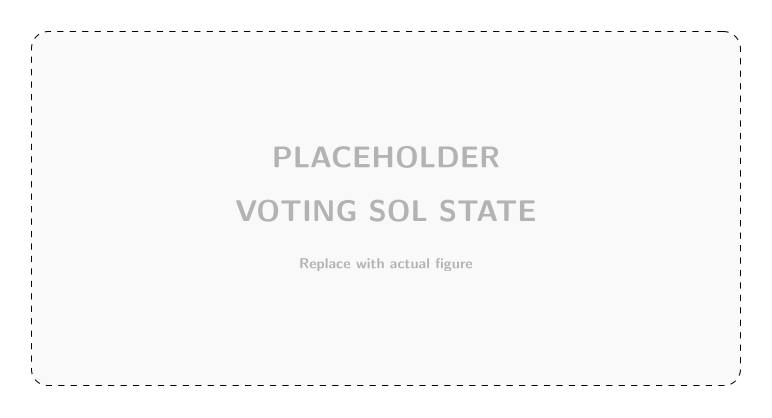
\includegraphics[width=0.85\textwidth]{Images/fig_voting_sol_state.png}
\caption{Voting.sol internal state machine with five verification checks during the vote function.}
\label{fig:voting-state-detail}
\end{figure}

\subsection{View Functions}

\begin{lstlisting}[language=Java, caption={Key view functions for state querying.}]
function getVotingData() external view returns (
    string memory question,
    address owner_addr,
    Phase phase,
    uint256 regEndTime,
    uint256 votEndTime,
    uint256 treeSize,
    uint256 depth,
    uint256 root,
    uint256 candidateCount
) {
    uint256 eid = s_electionId;
    return (
        s_question, owner(), _currentPhase(),
        s_registrationEndTime, s_votingEndTime,
        LeanIMT._size(s_trees[eid]),
        LeanIMT._depth(s_trees[eid]),
        s_trees[eid]._root(),
        s_candidates.length
    );
}

function isNullifierUsed(bytes32 _hash) 
    external view returns (bool) 
{
    return s_nullifierHashes[s_electionId][_hash];
}
\end{lstlisting}

\section{ElectionRegistry.sol: Factory Pattern and Aggregation}

\begin{figure}[H]
\centering
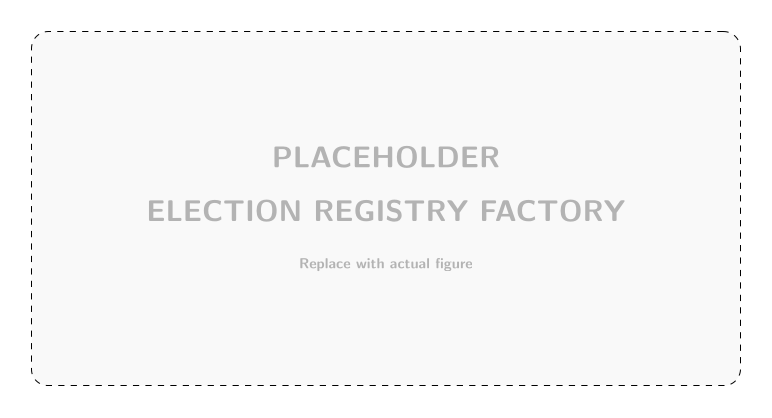
\includegraphics[width=0.85\textwidth]{Images/fig_election_registry_factory.png}
\caption{ElectionRegistry factory pattern: creates and manages 160 independent Voting contract instances with national result aggregation.}
\label{fig:registry-factory}
\end{figure}

\subsection{Division Structure}

\begin{lstlisting}[language=Java, caption={Division struct and state in ElectionRegistry.}]
struct Division {
    string name;              // e.g., "Kaduwela", "Colombo North"
    address votingContract;   // Deployed Voting.sol address
    address gnOfficer;        // Assigned GN officer
    bool active;              // Can be deactivated
}

Division[] public divisions;
address public immutable i_verifier;  // Shared HonkVerifier
\end{lstlisting}

\subsection{Factory Methods}

\begin{lstlisting}[language=Java, caption={Division creation via factory pattern.}]
function createDivision(string calldata name) 
    external onlyOwner 
    returns (uint256 divisionId, address votingContract)
{
    // Deploy fresh Voting instance with shared verifier
    Voting newVoting = new Voting(
        IHonkVerifier(i_verifier), msg.sender
    );
    
    divisions.push(Division({
        name: name,
        votingContract: address(newVoting),
        gnOfficer: address(0),
        active: true
    }));
    
    divisionId = divisions.length - 1;
    votingContract = address(newVoting);
    
    emit DivisionCreated(divisionId, name, votingContract);
}
\end{lstlisting}

\subsection{National Aggregation}

\begin{lstlisting}[language=Java, caption={National vote count aggregation across all active divisions.}]
function getNationalResults() 
    external view returns (uint256[] memory totals)
{
    // Determine max candidates across all divisions
    uint256 maxCandidates = 0;
    for (uint256 i = 0; i < divisions.length; i++) {
        if (!divisions[i].active) continue;
        uint256 count = Voting(divisions[i].votingContract)
            .getCandidates().length;
        if (count > maxCandidates) maxCandidates = count;
    }
    
    // Sum votes per candidate across all divisions
    totals = new uint256[](maxCandidates);
    for (uint256 i = 0; i < divisions.length; i++) {
        if (!divisions[i].active) continue;
        uint256[] memory divVotes = Voting(
            divisions[i].votingContract
        ).getVoteCounts();
        for (uint256 c = 0; c < divVotes.length; c++) {
            totals[c] += divVotes[c];
        }
    }
}
\end{lstlisting}

\section{NicRegistry.sol: Cross-Division Sybil Prevention}

\begin{figure}[H]
\centering
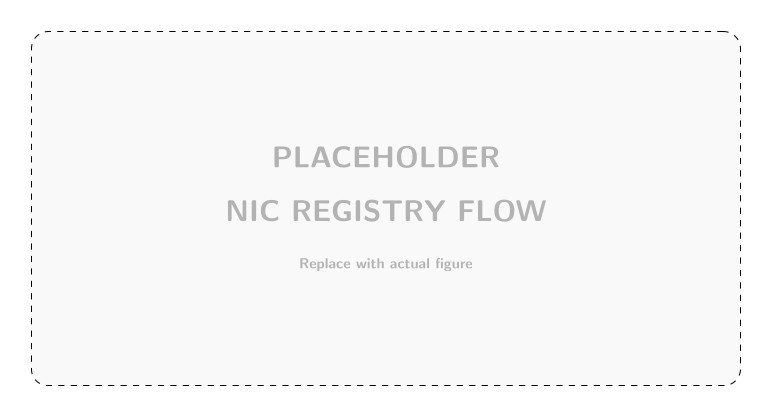
\includegraphics[width=0.85\textwidth]{Images/fig_nic_registry_flow.png}
\caption{NicRegistry flow: hashed NIC reservation prevents the same citizen from registering across multiple polling divisions.}
\label{fig:nic-flow}
\end{figure}

\subsection{Design Rationale}

A voter could potentially register in multiple divisions using different wallets. The NicRegistry prevents this by storing hashed National Identity Card numbers:

\begin{equation}
\text{nicHash} = \Poseidon(\text{NIC\_number}, \text{SERVER\_PEPPER})
\end{equation}

The server pepper is a secret known only to the election authority, preventing brute-force enumeration of NIC hashes from the public blockchain state.

\begin{lstlisting}[language=Java, caption={NicRegistry contract for cross-division Sybil prevention.}]
contract NicRegistry is Ownable {
    mapping(bytes32 => bool) private s_usedNicHashes;
    mapping(address => bool) private s_votingContracts;
    
    error NicRegistry__AlreadyUsed(bytes32 nicHash);
    event NicHashReserved(bytes32 indexed nicHash);
    
    function setVotingContract(
        address votingContract, bool authorized
    ) external onlyOwner {
        s_votingContracts[votingContract] = authorized;
    }
    
    function reserveNicHash(
        bytes32 nicHash, address votingContract
    ) external returns (bool) {
        // Only owner or GN of specified division can reserve
        require(
            msg.sender == owner() || 
            _isGNOf(msg.sender, votingContract),
            "Unauthorized"
        );
        
        if (s_usedNicHashes[nicHash])
            revert NicRegistry__AlreadyUsed(nicHash);
        
        s_usedNicHashes[nicHash] = true;
        emit NicHashReserved(nicHash);
        return true;
    }
}
\end{lstlisting}

\section{HonkVerifier.sol: Auto-Generated Proof Verifier}

The HonkVerifier is auto-generated by the Barretenberg compiler and contains:
\begin{itemize}
    \item Hardcoded verification key (circuit-specific polynomial commitments)
    \item Proof deserialization logic
    \item Fiat--Shamir transcript reconstruction
    \item BN254 pairing verification using precompile \texttt{0x08}
\end{itemize}

\begin{lstlisting}[language=Java, caption={HonkVerifier interface and key constants.}]
interface IHonkVerifier {
    function verify(
        bytes calldata _proof, 
        bytes32[] calldata _publicInputs
    ) external view returns (bool);
}

// Internal constants (from verification key)
uint256 constant N = 32768;
uint256 constant LOG_N = 15;
uint256 constant NUMBER_OF_PUBLIC_INPUTS = 4;
// Public inputs order: [nullifierHash, root, vote, depth]
\end{lstlisting}

\section{Deployment Pipeline}

The contracts must be deployed in strict dependency order:

\begin{enumerate}
    \item \texttt{PoseidonT3} library (used by LeanIMT)
    \item \texttt{LeanIMT} library (linked into Voting)
    \item \texttt{HonkVerifier} (standalone, no dependencies)
    \item \texttt{Voting} (references HonkVerifier address)
    \item \texttt{ElectionRegistry} (references HonkVerifier, deploys Voting instances)
    \item \texttt{NicRegistry} (standalone, references Voting contracts post-deploy)
\end{enumerate}

Library linking is required because Solidity libraries with external functions must be deployed separately and their addresses embedded in the calling contract's bytecode at deploy time.

\section{Custom Go Blockchain Architecture}

\begin{figure}[H]
\centering
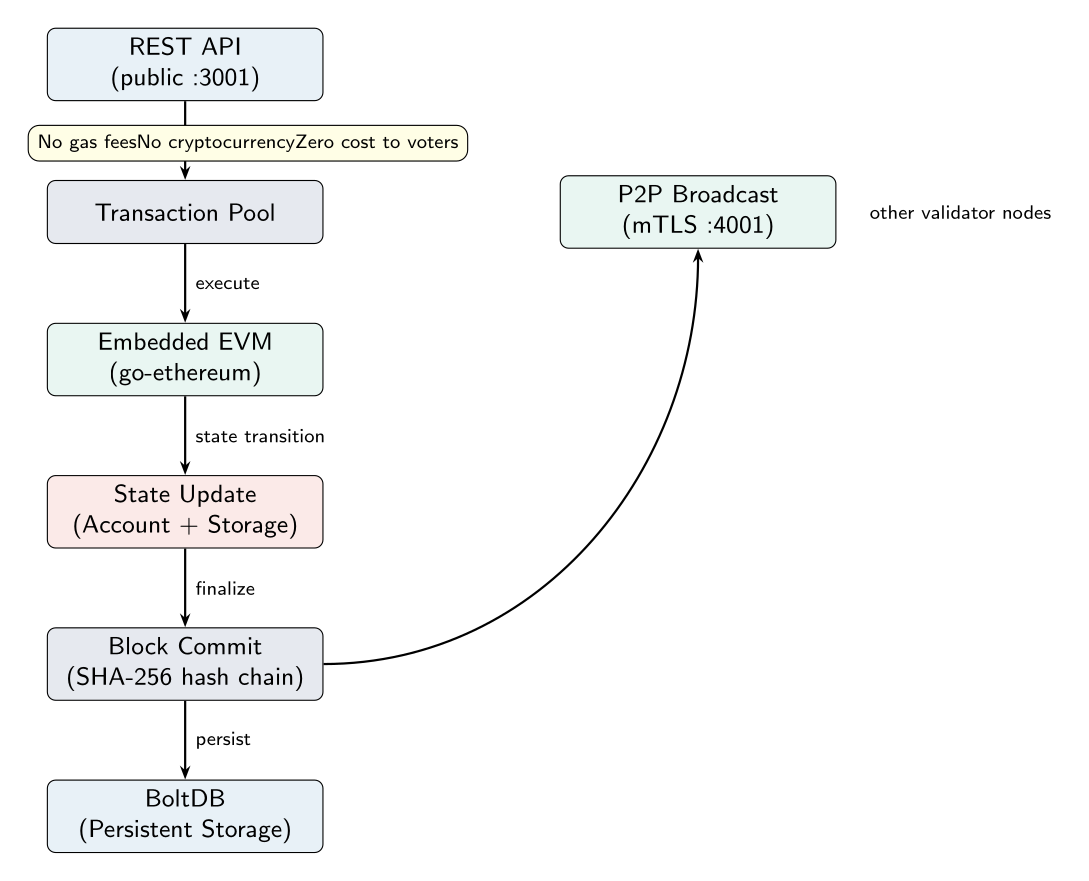
\includegraphics[width=0.85\textwidth]{Images/fig_go_blockchain.png}
\caption{Custom Go blockchain architecture showing the six internal packages and their interactions.}
\label{fig:go-blockchain}
\end{figure}

\subsection{Package Organization}

\begin{table}[H]
\centering
\caption{Go blockchain internal package structure.}
\label{tab:go-packages}
\begin{tabular}{|l|p{8cm}|}
\hline
\textbf{Package} & \textbf{Responsibility} \\
\hline
\texttt{internal/core} & Blockchain data structures: Transaction, Block, Blockchain types \\
\hline
\texttt{internal/evm} & Embedded go-ethereum EVM: StateDB, contract execution, precompiles \\
\hline
\texttt{internal/api} & HTTP handlers, middleware, routing (public + P2P listeners) \\
\hline
\texttt{internal/network} & Peer discovery, mTLS broadcast, periodic state synchronization \\
\hline
\texttt{internal/persistence} & BoltDB on-disk block and state storage \\
\hline
\texttt{internal/security} & RSA admin authentication, mTLS certificate management \\
\hline
\end{tabular}
\end{table}

\subsection{Gasless Execution Model}

\begin{lstlisting}[language=Java, caption={Gasless EVM execution in Go (simplified).}]
func (e *EVMExecutor) ExecuteCall(
    from, to common.Address,
    data []byte,
) ([]byte, error) {
    // Set gas limit but never deduct cost
    gasLimit := uint64(16_000_000)
    
    // Create EVM with current state
    evm := vm.NewEVM(
        e.blockContext(),
        vm.TxContext{Origin: from},
        e.stateDB,
        e.chainConfig,
        vm.Config{},
    )
    
    // Execute (gas metered for DoS protection only)
    ret, remainingGas, err := evm.Call(
        vm.AccountRef(from), to, data, gasLimit,
        new(uint256.Int), // value = 0 (gasless)
    )
    
    // Commit state changes (no gas deduction)
    e.stateDB.Commit()
    return ret, err
}
\end{lstlisting}

\subsection{Block Structure}

\begin{lstlisting}[language=Java, caption={Block and Transaction structures in Go.}]
type Transaction struct {
    ID        string    `json:"id"`
    Type      string    `json:"type"`      // "register", "vote", "admin"
    From      string    `json:"from"`
    To        string    `json:"to"`
    Data      []byte    `json:"data"`
    Timestamp time.Time `json:"timestamp"`
}

type Block struct {
    Index        uint64        `json:"index"`
    Timestamp    time.Time     `json:"timestamp"`
    Transactions []Transaction `json:"transactions"`
    PrevHash     string        `json:"prev_hash"`
    Hash         string        `json:"hash"`
    Validator    string        `json:"validator"`
}
\end{lstlisting}

\section{REST API Specification}

\begin{figure}[H]
\centering
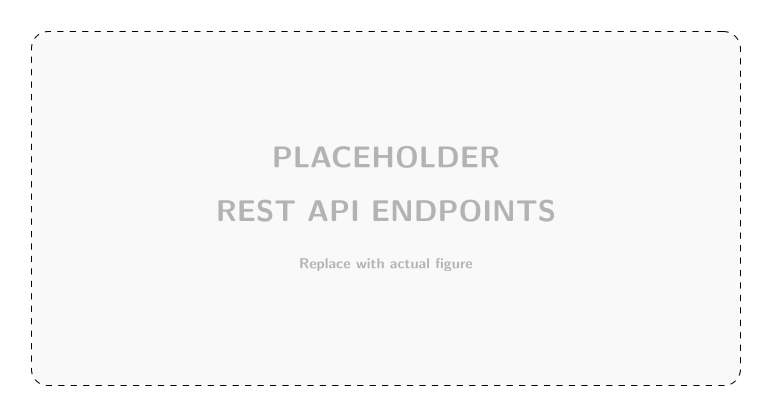
\includegraphics[width=0.85\textwidth]{Images/fig_rest_api_endpoints.png}
\caption{REST API endpoint map showing public (read), voter (rate-limited), and admin (RSA-signed) categories.}
\label{fig:rest-api}
\end{figure}

\subsection{Public Read Endpoints}

\begin{table}[H]
\centering
\caption{Public API endpoints (no authentication required).}
\label{tab:public-api}
\begin{tabular}{|l|l|p{5cm}|}
\hline
\textbf{Method} & \textbf{Endpoint} & \textbf{Response} \\
\hline
GET & \texttt{/voting-data} & Current election state, phases, tree info \\
\hline
GET & \texttt{/candidates} & Candidate name array \\
\hline
GET & \texttt{/vote-counts} & Per-candidate vote tallies \\
\hline
GET & \texttt{/voter/\{id\}} & Voter allowlist and registration status \\
\hline
GET & \texttt{/commitments} & All registered commitments (Merkle leaves) \\
\hline
GET & \texttt{/chain} & Full blockchain (all blocks) \\
\hline
GET & \texttt{/blocks?page=\&limit=} & Paginated block history \\
\hline
GET & \texttt{/health} & Node health status \\
\hline
\end{tabular}
\end{table}

\subsection{Voter Endpoints (Rate Limited)}

Rate limited to 1 request/second with burst of 5:

\begin{table}[H]
\centering
\caption{Voter-facing endpoints with rate limiting.}
\label{tab:voter-api}
\begin{tabular}{|l|l|p{5cm}|}
\hline
\textbf{Method} & \textbf{Endpoint} & \textbf{Action} \\
\hline
POST & \texttt{/register} & Submit commitment for Merkle tree insertion \\
\hline
POST & \texttt{/vote} & Submit ZK proof and anonymous vote \\
\hline
\end{tabular}
\end{table}

\subsection{Admin Endpoints (RSA Authenticated)}

\begin{table}[H]
\centering
\caption{Admin API endpoints requiring RSA signature authentication.}
\label{tab:admin-api}
\begin{tabular}{|l|l|p{5cm}|}
\hline
\textbf{Method} & \textbf{Endpoint} & \textbf{Action} \\
\hline
POST & \texttt{/add-voter} & Add voter to allowlist \\
\hline
POST & \texttt{/set-question} & Set ballot question \\
\hline
POST & \texttt{/set-candidates} & Set candidate list \\
\hline
POST & \texttt{/start-registration} & Begin registration phase \\
\hline
POST & \texttt{/start-voting} & Begin voting phase \\
\hline
POST & \texttt{/end-election} & End election early \\
\hline
POST & \texttt{/reset-election} & Reset to setup phase \\
\hline
\end{tabular}
\end{table}

\section{Admin RSA Authentication}

\begin{lstlisting}[language=Java, caption={RSA signature verification for admin endpoints.}]
// Admin request authentication:
// Header: X-Admin-Signature = base64(RSA-SHA256(message))
// Header: X-Admin-Timestamp = unix_seconds
// Message = "<timestamp>\n<path>\n<body>"
// Time window: +/- 5 minutes

func verifyAdminSignature(r *http.Request) error {
    sig := r.Header.Get("X-Admin-Signature")
    ts := r.Header.Get("X-Admin-Timestamp")
    
    // Check timestamp within 5-minute window
    reqTime, _ := strconv.ParseInt(ts, 10, 64)
    if abs(time.Now().Unix()-reqTime) > 300 {
        return errors.New("timestamp expired")
    }
    
    // Reconstruct signed message
    body, _ := io.ReadAll(r.Body)
    message := fmt.Sprintf("%s\n%s\n%s", ts, r.URL.Path, body)
    
    // Verify RSA-SHA256 PKCS#1 v1.5 signature
    hash := sha256.Sum256([]byte(message))
    return rsa.VerifyPKCS1v15(adminPubKey, crypto.SHA256, hash[:], sigBytes)
}
\end{lstlisting}

\section{PBFT Consensus}

\begin{figure}[H]
\centering
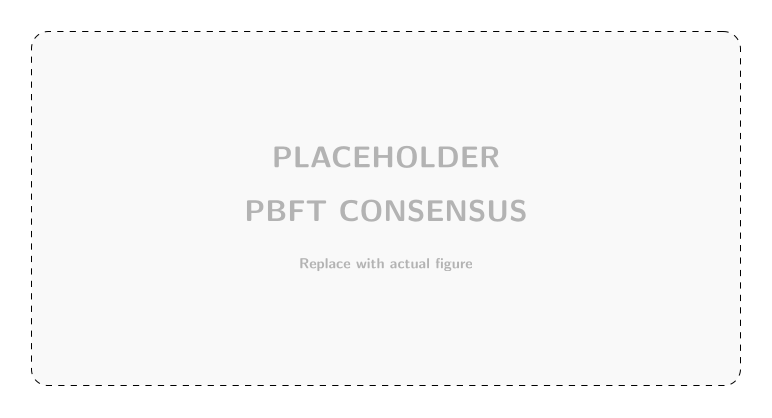
\includegraphics[width=0.85\textwidth]{Images/fig_pbft_consensus.png}
\caption{PBFT consensus flow among election commission validator nodes: pre-prepare, prepare, commit phases.}
\label{fig:pbft}
\end{figure}

Our PBFT implementation provides:
\begin{itemize}
    \item \textbf{Fault tolerance}: Tolerates $f < n/3$ Byzantine nodes
    \item \textbf{Deterministic finality}: No block reorgs possible
    \item \textbf{Geographic distribution}: Nodes in different election commission offices
    \item \textbf{mTLS communication}: All inter-node traffic encrypted and authenticated
\end{itemize}

\section{BoltDB Persistence}

\begin{lstlisting}[language=Java, caption={BoltDB block persistence layer.}]
// Buckets:
// "blocks"     -> block_index (uint64 BE) -> Block JSON
// "state"      -> "latest_index" -> uint64
// "accounts"   -> address -> Account JSON
// "storage"    -> address+slot -> value

func (p *Persistence) StoreBlock(block *Block) error {
    return p.db.Update(func(tx *bolt.Tx) error {
        b := tx.Bucket([]byte("blocks"))
        key := uint64ToBytes(block.Index)
        data, _ := json.Marshal(block)
        return b.Put(key, data)
    })
}
\end{lstlisting}

\begin{figure}[H]
\centering
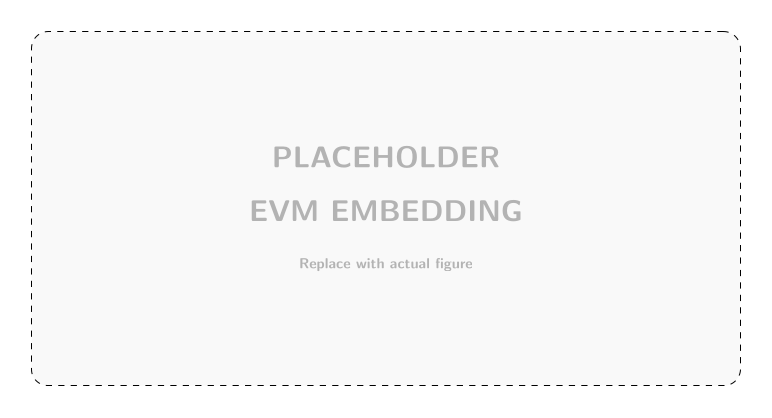
\includegraphics[width=0.85\textwidth]{Images/fig_evm_embedding.png}
\caption{EVM embedding architecture: Go blockchain wraps go-ethereum's VM package with a custom StateDB backed by BoltDB.}
\label{fig:evm-embed}
\end{figure}

\section{Summary}

This chapter has presented the complete smart contract layer (Voting.sol, ElectionRegistry.sol, NicRegistry.sol, HonkVerifier.sol) and custom Go blockchain implementation. The contracts implement a rigorous state machine with five-layer fraud prevention, while the blockchain provides gasless execution, PBFT consensus, and RSA-authenticated administration. Together, they form the trusted execution layer that our application interfaces (Chapter~\ref{ch:applications}) interact with through well-defined APIs.

\chapter{Application Development}\label{ch:applications}

This chapter details the development of our two application frontends: the React Native mobile voting app (for citizens) and the Next.js web application (for administrators, GN officers, and public observers). We describe the architecture of each, focusing on the security-critical flows: hardware keystore management, biometric authentication, on-device proof generation, and the three-factor voting protocol.

\section{Mobile Application Architecture}

\subsection{Technology Stack}

\begin{table}[H]
\centering
\caption{Mobile application technology stack.}
\label{tab:mobile-stack}
\begin{tabular}{|l|l|l|}
\hline
\textbf{Component} & \textbf{Technology} & \textbf{Version} \\
\hline
Framework & React Native & 0.81.5 \\
\hline
Platform & Expo & SDK 54 \\
\hline
JS Engine & Hermes & (bundled) \\
\hline
Routing & Expo Router & v6 \\
\hline
EVM Interaction & viem & 2.21.0 \\
\hline
Cryptography & poseidon-lite & 0.3.0 \\
\hline
Key Storage & expo-secure-store & 15.0.8 \\
\hline
Biometrics & expo-local-authentication & 17.0.8 \\
\hline
QR Display & react-native-qrcode-svg & 6.3.2 \\
\hline
Merkle Tree & @zk-kit/lean-imt & 2.2.4 \\
\hline
\end{tabular}
\end{table}

\subsection{Screen Architecture}

The mobile app uses Expo Router's file-based routing:

\begin{figure}[H]
\centering
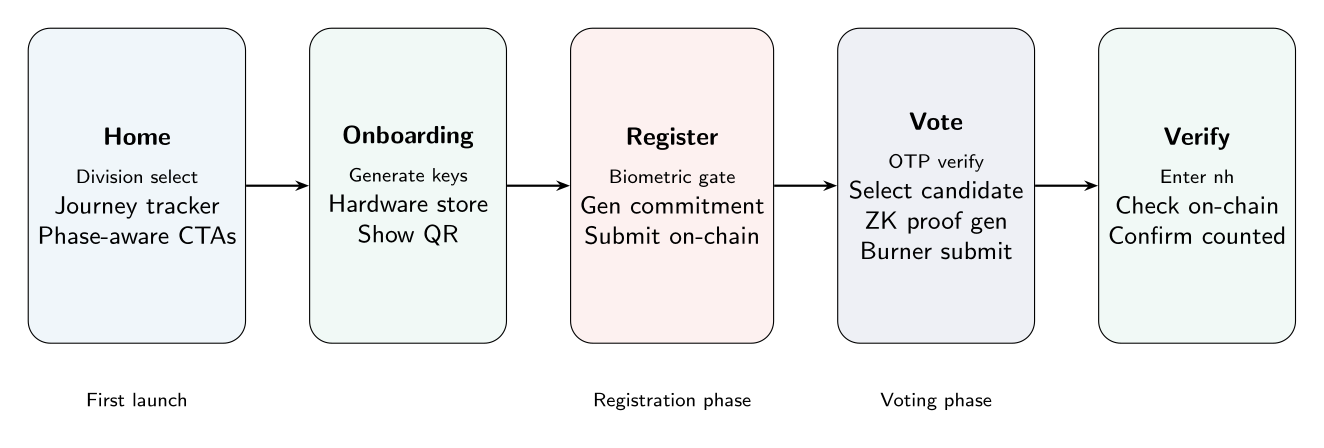
\includegraphics[width=0.85\textwidth]{Images/fig_mobile_flow.png}
\caption{Mobile app screen flow: from onboarding through registration to voting, with security gates at each transition.}
\label{fig:mobile-flow}
\end{figure}

\begin{table}[H]
\centering
\caption{Mobile app screen inventory.}
\label{tab:mobile-screens}
\begin{tabular}{|l|l|p{5cm}|}
\hline
\textbf{Route} & \textbf{Screen} & \textbf{Function} \\
\hline
\texttt{/} & Home & Division selector, journey tracker, action buttons \\
\hline
\texttt{/onboarding} & Onboarding & Identity creation (key generation) \\
\hline
\texttt{/register} & Registration & Biometric $\to$ Commitment $\to$ On-chain register \\
\hline
\texttt{/vote} & Voting & OTP $\to$ Biometric $\to$ Candidate $\to$ Proof $\to$ Submit \\
\hline
\texttt{/verify} & Verification & Check vote by nullifier hash \\
\hline
\texttt{/settings} & Settings & App configuration \\
\hline
\end{tabular}
\end{table}

\section{Hardware Keystore Implementation}

\subsection{Secure Storage Architecture}

\begin{figure}[H]
\centering
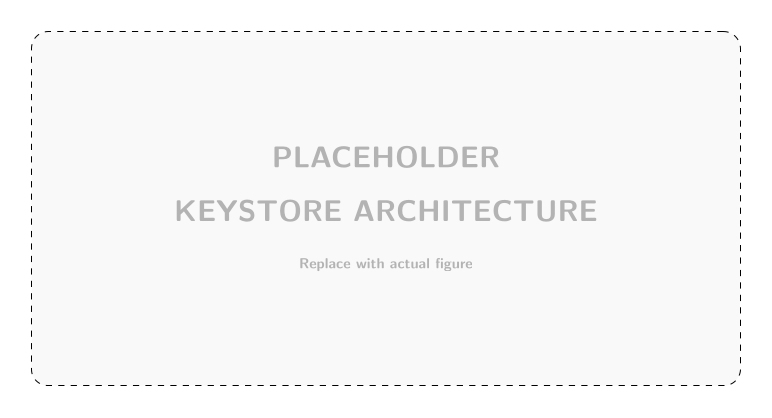
\includegraphics[width=0.85\textwidth]{Images/fig_keystore_architecture.png}
\caption{Hardware keystore architecture: sensitive secrets (private key, nullifier, secret) require biometric authentication; public data (address, flags) does not.}
\label{fig:keystore}
\end{figure}

The keystore separates items into two security tiers:

\begin{table}[H]
\centering
\caption{Keystore items with authentication requirements.}
\label{tab:keystore-items}
\begin{tabular}{|l|l|l|p{4cm}|}
\hline
\textbf{Key} & \textbf{Auth Gated} & \textbf{Type} & \textbf{Purpose} \\
\hline
\texttt{slvote.privateKey} & Yes (biometric) & Hex string & EVM transaction signing \\
\hline
\texttt{slvote.nullifier} & Yes (biometric) & Field element & ZK commitment secret \\
\hline
\texttt{slvote.secret} & Yes (biometric) & Field element & ZK commitment secret \\
\hline
\texttt{slvote.address} & No & Hex string & Public wallet address \\
\hline
\texttt{slvote.division} & No & Address & Selected division contract \\
\hline
\texttt{slvote.registered} & No & Boolean & Registration status flag \\
\hline
\texttt{slvote.voted} & No & JSON array & Divisions voted in \\
\hline
\end{tabular}
\end{table}

\subsection{Implementation Details}

\begin{lstlisting}[language=Java, caption={Keystore implementation with biometric gating.}]
import * as SecureStore from 'expo-secure-store';
import { Platform } from 'react-native';

const isExpoGo = Constants.appOwnership === 'expo';

const AUTH_OPTIONS: SecureStoreOptions = {
  requireAuthentication: !isExpoGo,
  authenticationPrompt: "Unlock your voting identity",
  keychainAccessible: 
    SecureStore.WHEN_UNLOCKED_THIS_DEVICE_ONLY,
};

// Biometric-gated access to private key
export async function getPrivateKey(): Promise<`0x${string}`> {
  const pk = await SecureStore.getItemAsync(
    'slvote.privateKey', AUTH_OPTIONS
  );
  if (!pk) throw new Error('No identity found');
  return pk as `0x${string}`;
}

// Public access (no biometric prompt)
export async function getAddress(): Promise<`0x${string}`> {
  const addr = await SecureStore.getItemAsync('slvote.address');
  return addr as `0x${string}`;
}
\end{lstlisting}

\subsection{Identity Creation}

\begin{lstlisting}[language=Java, caption={One-time identity creation during onboarding.}]
export async function createIdentity(): Promise<`0x${string}`> {
  // Generate cryptographic keypair
  const privateKey = generatePrivateKey(); // viem
  const address = privateKeyToAddress(privateKey);
  
  // Store with biometric protection
  await SecureStore.setItemAsync(
    'slvote.privateKey', privateKey, AUTH_OPTIONS
  );
  await SecureStore.setItemAsync('slvote.address', address);
  
  return address;
}
\end{lstlisting}

\section{Biometric Authentication Flow}

\begin{figure}[H]
\centering
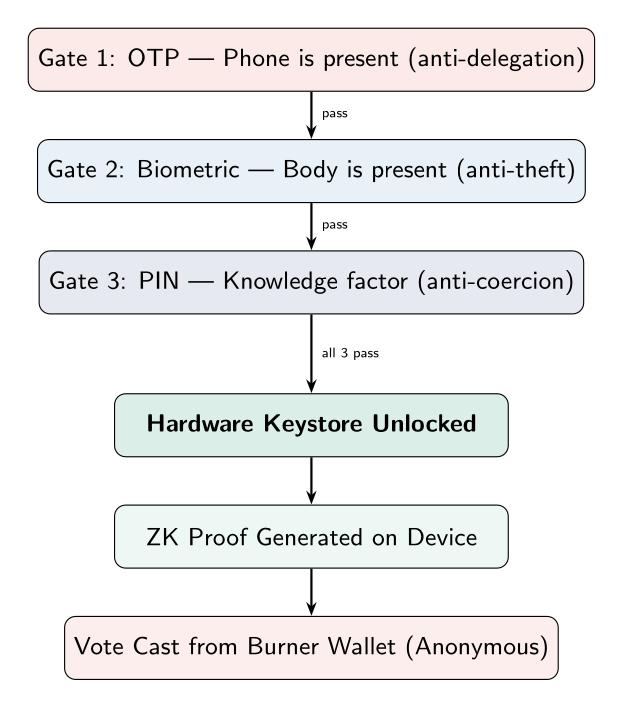
\includegraphics[width=0.85\textwidth]{Images/fig_auth.png}
\caption{Biometric authentication flow: capability check, enrollment verification, and hardware-backed prompt.}
\label{fig:auth-flow}
\end{figure}

\begin{lstlisting}[language=Java, caption={Biometric authentication with capability detection.}]
import * as LocalAuthentication from 'expo-local-authentication';

export async function authenticate(
  reason: string = "Verify your identity"
): Promise<boolean> {
  // Check hardware capability
  const hasHardware = await LocalAuthentication
    .hasHardwareAsync();
  if (!hasHardware) return false;
  
  // Check enrollment
  const isEnrolled = await LocalAuthentication
    .isEnrolledAsync();
  if (!isEnrolled) return false;
  
  // Prompt user
  const result = await LocalAuthentication
    .authenticateAsync({
      promptMessage: reason,
      fallbackLabel: "Use PIN",
      disableDeviceFallback: false,
    });
  
  return result.success;
}

export async function getBiometricCapability() {
  return {
    hasHardware: await LocalAuthentication.hasHardwareAsync(),
    isEnrolled: await LocalAuthentication.isEnrolledAsync(),
    supported: await LocalAuthentication
      .supportedAuthenticationTypesAsync(),
  };
}
\end{lstlisting}

\section{Commitment Cryptography}

\begin{lstlisting}[language=Java, caption={Voter commitment generation using Poseidon.}]
import { poseidon1, poseidon2 } from 'poseidon-lite';

const FIELD_PRIME = 21888242871839275222246405745257275088
  548364400416034343698204186575808495617n;

function randomFieldElement(): bigint {
  const bytes = crypto.getRandomValues(new Uint8Array(32));
  const num = BigInt('0x' + Buffer.from(bytes).toString('hex'));
  return num % FIELD_PRIME;
}

export interface VoterCommitment {
  nullifier: string;
  secret: string;
  commitment: string;
  nullifierHash: string;
}

export function generateCommitment(): VoterCommitment {
  const nullifier = randomFieldElement();
  const secret = randomFieldElement();
  const commitment = poseidon2([nullifier, secret]);
  const nullifierHash = poseidon1([nullifier]);
  
  return {
    nullifier: nullifier.toString(),
    secret: secret.toString(),
    commitment: commitment.toString(),
    nullifierHash: nullifierHash.toString(),
  };
}
\end{lstlisting}

\section{ZK Proof Generation on Mobile}

\subsection{WebView-Based Proving}

Due to Hermes's lack of BigInt support, ZK proof generation runs inside a React Native WebView that uses the device's system WebKit/Chromium engine (which supports BigInt natively):

\begin{lstlisting}[language=Java, caption={WebView proof generation architecture.}]
// React Native side: pass witness to WebView
const generateProof = async (inputs: CircuitInputs) => {
  return new Promise((resolve) => {
    webviewRef.current.postMessage(JSON.stringify({
      type: 'GENERATE_PROOF',
      inputs: inputs,
    }));
    
    // WebView will respond via onMessage
    onMessageRef.current = (event) => {
      const data = JSON.parse(event.nativeEvent.data);
      if (data.type === 'PROOF_RESULT') {
        resolve(data.proof);
      }
    };
  });
};

// WebView HTML (runs in system V8/JSCore):
// - Loads bb.js WASM module
// - Loads compiled ACIR circuit
// - Receives witness via postMessage
// - Generates UltraHonk proof
// - Returns proof bytes via postMessage
\end{lstlisting}

\subsection{Witness Construction}

\begin{lstlisting}[language=Java, caption={Circuit witness construction from voter secrets and chain state.}]
interface VoteProofParams {
  nullifier: string;
  secret: string;
  circuitIndex: string;   // Leaf index in tree
  siblings: string[];     // 16-element Merkle path
  root: string;           // Current tree root
  candidateIndex: number; // User's candidate choice
  depth: number;          // Current tree depth
}

function buildCircuitInputs(params: VoteProofParams): CircuitInputs {
  const nullifier = BigInt(params.nullifier);
  const nullifierHash = poseidon1([nullifier]);
  
  // Pad siblings to 16 elements
  const paddedSiblings = [...params.siblings];
  while (paddedSiblings.length < 16) {
    paddedSiblings.push("0");
  }
  
  return {
    nullifier_hash: nullifierHash.toString(),
    root: params.root,
    vote: params.candidateIndex.toString(),
    depth: params.depth.toString(),
    nullifier: params.nullifier,
    secret: params.secret,
    index: params.circuitIndex,
    siblings: paddedSiblings,
  };
}
\end{lstlisting}

\section{Chain Interaction: Legacy Transaction Signing}

\begin{lstlisting}[language=Java, caption={Manual legacy transaction signing for Hermes compatibility.}]
import { 
  encodeFunctionData, createWalletClient, http 
} from 'viem';

export async function submitVote(
  divisionContract: `0x${string}`,
  callData: VoteCallData,
  burnerPrivateKey: `0x${string}`,
): Promise<`0x${string}`> {
  // Encode vote function call
  const data = encodeFunctionData({
    abi: VotingABI,
    functionName: 'vote',
    args: [
      callData.proof,
      callData.nullifierHash,
      callData.root,
      callData.vote,
      callData.depth,
    ],
  });
  
  // Manual legacy tx (avoids BigInt gas estimation)
  const client = createWalletClient({
    account: privateKeyToAccount(burnerPrivateKey),
    transport: http(RPC_URL),
  });
  
  return client.sendTransaction({
    to: divisionContract,
    data: data,
    gas: 500000n,     // Fixed gas limit
    gasPrice: 0n,     // Gasless chain
    type: 'legacy',   // Avoid EIP-1559 BigInt issues
  });
}
\end{lstlisting}

\section{Three-Factor Voting Authentication}

The voting flow requires three independent authentication factors:

\begin{enumerate}
    \item \textbf{Factor 1: OTP Phone Verification}
    \begin{itemize}
        \item Voter enters phone number
        \item Server sends SMS OTP (6-digit code)
        \item Voter enters code within time window
        \item Prevents bot-based automated voting
    \end{itemize}
    
    \item \textbf{Factor 2: Biometric Authentication}
    \begin{itemize}
        \item Device fingerprint sensor or face recognition
        \item Hardware-backed (TEE/Secure Enclave)
        \item Unlocks access to voter secrets in keystore
        \item Proves physical possession of enrolled device
    \end{itemize}
    
    \item \textbf{Factor 3: Cryptographic Identity (Hardware PIN)}
    \begin{itemize}
        \item Private key stored in hardware keystore
        \item Only accessible after biometric + device PIN
        \item Used to sign the registration transaction
        \item Proves ownership of the registered commitment
    \end{itemize}
\end{enumerate}

\section{Burner Wallet Mechanism}

To achieve voter--ballot unlinkability, votes are submitted from ephemeral ``burner'' wallets:

\begin{lstlisting}[language=Java, caption={Burner wallet creation and usage.}]
export function newBurnerAccount() {
  const privateKey = generatePrivateKey();
  const address = privateKeyToAddress(privateKey);
  return { privateKey, address };
}

// Voting flow:
// 1. Generate fresh burner (no prior history)
// 2. Fund burner via faucet/paymaster (small amount for gas)
// 3. Submit vote from burner address
// 4. Discard burner private key (never stored)
\end{lstlisting}

\textbf{Key property}: The burner address has no transaction history linking it to the voter's registered address. Even if an observer correlates the faucet funding, the ZK proof prevents linking the proof to a specific voter identity.

\section{Next.js Web Application}

\subsection{Routes and Access Control}

\begin{table}[H]
\centering
\caption{Next.js web application routes.}
\label{tab:web-routes}
\begin{tabular}{|l|l|l|}
\hline
\textbf{Route} & \textbf{Purpose} & \textbf{Access} \\
\hline
\texttt{/} & Landing page & Public \\
\hline
\texttt{/voting} & Mobile download prompt & Public \\
\hline
\texttt{/voting/admin} & Election Authority dashboard & Admin wallet \\
\hline
\texttt{/voting/admin/[id]} & Division management & Admin wallet \\
\hline
\texttt{/gn} & Grama Niladhari portal & GN wallet \\
\hline
\texttt{/gn/register} & Voter enrollment & GN wallet \\
\hline
\texttt{/results} & Live election results & Public \\
\hline
\texttt{/audit} & Observer verification & Public \\
\hline
\texttt{/debug} & Contract debugging (dev only) & Dev \\
\hline
\end{tabular}
\end{table}

\subsection{Admin Dashboard}

\begin{figure}[H]
\centering
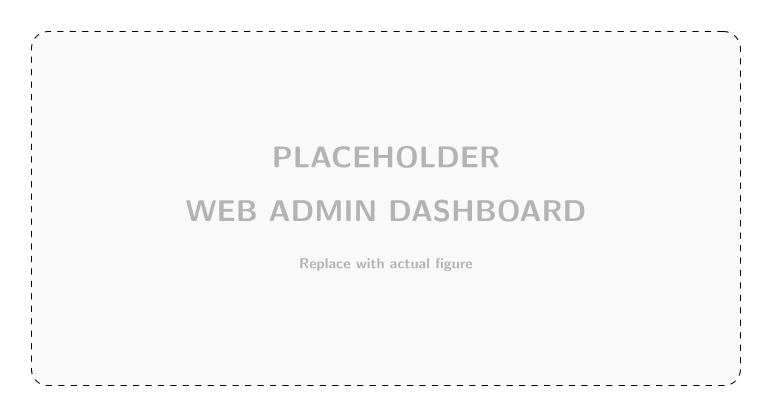
\includegraphics[width=0.85\textwidth]{Images/fig_web_admin_dashboard.png}
\caption{Web admin dashboard: division management, phase control, and national overview.}
\label{fig:admin-dashboard}
\end{figure}

The admin dashboard provides:
\begin{itemize}
    \item \textbf{Division Management}: Create divisions, assign GN officers, view per-division status
    \item \textbf{Election Setup}: Set ballot question, configure candidates (up to 100)
    \item \textbf{Phase Control}: Start registration/voting with configurable durations
    \item \textbf{National Overview}: Aggregate statistics across all 160 divisions
\end{itemize}

\subsection{GN Officer Portal}

\begin{figure}[H]
\centering
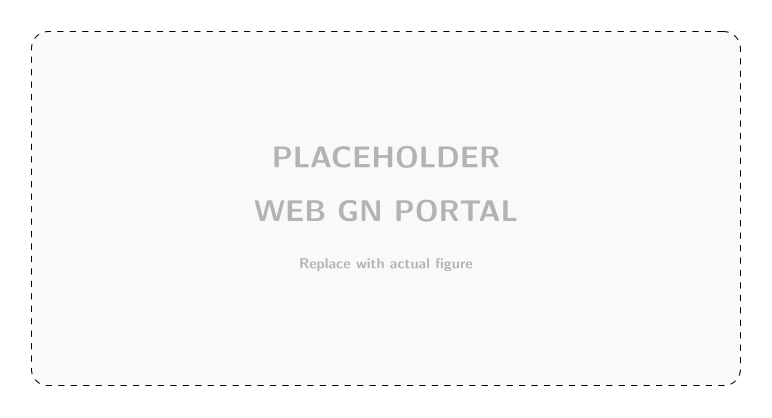
\includegraphics[width=0.85\textwidth]{Images/fig_web_gn_portal.png}
\caption{GN Officer portal: voter enrollment interface with QR scanning and NIC verification.}
\label{fig:gn-portal}
\end{figure}

The GN portal enables village officers to:
\begin{itemize}
    \item View their assigned division and its current phase
    \item Add voters to the allowlist (batch or individual)
    \item Monitor registration progress (tree size, voter list)
    \item Reserve NIC hashes for cross-division de-duplication
    \item Scan voter QR codes for identity verification
\end{itemize}

\subsection{Results Page and National Aggregation}

\begin{figure}[H]
\centering
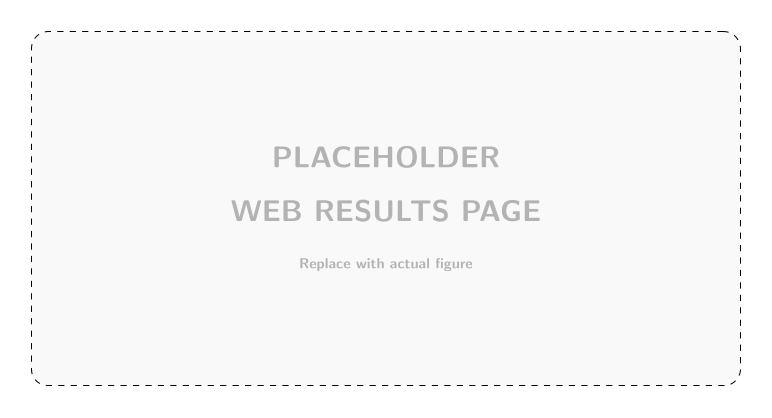
\includegraphics[width=0.85\textwidth]{Images/fig_web_results_page.png}
\caption{Public results page: national vote totals with per-division breakdown and live updating.}
\label{fig:results-page}
\end{figure}

The results page provides:
\begin{itemize}
    \item National vote totals (pie chart + bar chart)
    \item Per-division breakdown (searchable table)
    \item Real-time polling (auto-refresh every 10 seconds)
    \item CSV export for independent analysis
    \item Turnout statistics (registered vs. voted)
\end{itemize}

\subsection{Dual Backend Architecture}

The web application supports two backends transparently:

\begin{lstlisting}[language=Java, caption={Backend-agnostic service layer configuration.}]
// scaffold.config.ts
const scaffoldConfig = {
  chainBackend: process.env.NEXT_PUBLIC_CHAIN_BACKEND 
    as "hardhat" | "custom",
  targetNetworks: [chains.hardhat],
  chainApiUrl: process.env.NEXT_PUBLIC_CHAIN_API_URL 
    || "http://localhost:3001",
};
\end{lstlisting}

\begin{table}[H]
\centering
\caption{Dual backend comparison: Hardhat vs. Custom Go blockchain.}
\label{tab:dual-backend}
\begin{tabular}{|l|l|l|}
\hline
\textbf{Aspect} & \textbf{Hardhat Backend} & \textbf{Custom Backend} \\
\hline
RPC & \texttt{localhost:8545} & \texttt{localhost:3001} (REST) \\
\hline
Voter ID & Ethereum address & String ID (email/phone) \\
\hline
Vote submission & Signed EVM tx & Unsigned POST /vote \\
\hline
Gas model & Standard gas & Gasless (free) \\
\hline
Admin auth & Contract ownership & RSA signature \\
\hline
\end{tabular}
\end{table}

This architecture allows development and testing on Hardhat (familiar tooling, fast iteration) while deploying to the custom blockchain for production (gasless, sovereign).

\section{Summary}

This chapter has detailed the complete application layer: a React Native mobile app with hardware-backed security, biometric authentication, and on-device ZK proof generation; and a Next.js web application with role-based access control for administrators, GN officers, and public observers. The three-factor authentication protocol (OTP + biometric + cryptographic identity) provides defense in depth for the voting action, while the burner wallet mechanism ensures voter--ballot unlinkability at the network layer. Chapter~\ref{ch:testing} evaluates the complete system's performance, security, and correctness through comprehensive testing.

\chapter{Testing, Results, and Evaluation}\label{ch:testing}

This chapter presents the comprehensive testing methodology, test results, performance characteristics, gas analysis, security evaluation, and comparative analysis of our system. We evaluate the system against its stated objectives and compare it with existing solutions.

\section{Testing Methodology}

Our testing strategy follows a four-tier approach:

\begin{enumerate}
    \item \textbf{Unit Testing}: Individual contract functions, circuit constraints, and blockchain node packages
    \item \textbf{Integration Testing}: Cross-component interactions (circuit $\to$ verifier $\to$ contract; deploy pipeline $\to$ node)
    \item \textbf{End-to-End Testing}: Complete voting flow (mobile $\to$ API $\to$ chain $\to$ verification)
    \item \textbf{Security Testing}: Adversarial inputs, edge cases, attack simulations
\end{enumerate}

A distinctive fifth technique applies to the custom blockchain: \textbf{differential testing}, in which identical JSON-RPC requests are issued to both a reference Hardhat node and our Go node, and the responses are compared field by field (Section~\ref{sec:chain-verification}).

\subsection{Testing Tools}

\begin{table}[H]
\centering
\caption{Testing tools and frameworks used.}
\label{tab:test-tools}
\begin{tabular}{|l|l|l|}
\hline
\textbf{Component} & \textbf{Framework} & \textbf{Coverage} \\
\hline
Smart Contracts & Hardhat + Chai + Ethers.js & 55 test cases \\
\hline
ZK Circuit & Nargo execute + bb prove/verify & Constraint verification \\
\hline
Custom Blockchain & Go testing + differential harness & Unit + RPC parity \\
\hline
Mobile App & Manual integration testing & Full flow validation \\
\hline
\end{tabular}
\end{table}

\section{Smart Contract Test Suite}

\subsection{Test Organization}

Our 55 unit tests are organized into logical groups across three test files:

\begin{figure}[H]
\centering
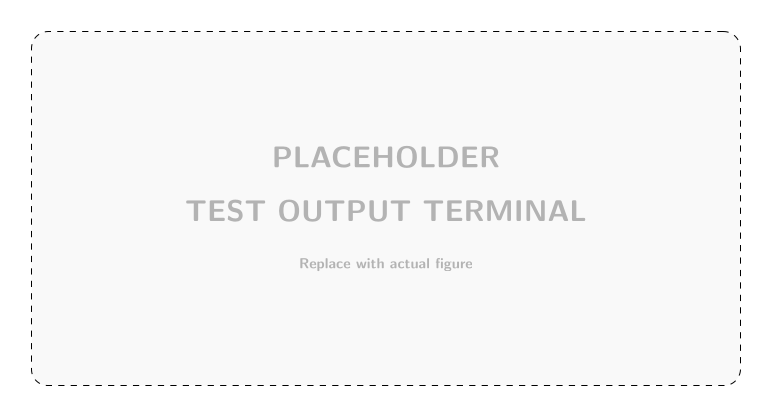
\includegraphics[width=0.85\textwidth]{Images/fig_test_output_terminal.png}
\caption{Terminal output showing all 55 tests passing across the Voting, GN officer/ElectionRegistry, and NicRegistry test suites.}
\label{fig:test-output}
\end{figure}

\begin{table}[H]
\centering
\caption{Test case distribution across contract modules.}
\label{tab:test-distribution}
\begin{tabular}{|l|r|l|}
\hline
\textbf{Test Group} & \textbf{Count} & \textbf{File} \\
\hline
Setup Phase & 8 & Voting.ts \\
\hline
Registration Phase & 10 & Voting.ts \\
\hline
Phase Transitions & 6 & Voting.ts \\
\hline
View Functions & 4 & Voting.ts \\
\hline
Reset / Multi-Election & 9 & Voting.ts \\
\hline
GN Officer Management & 7 & GNAndRegistry.ts \\
\hline
ElectionRegistry & 6 & GNAndRegistry.ts \\
\hline
NicRegistry & 5 & NicRegistry.ts \\
\hline
\textbf{Total} & \textbf{55} & \\
\hline
\end{tabular}
\end{table}

The \texttt{vote()} function's proof-dependent paths are deliberately \emph{not} unit-tested with fabricated proofs---a valid UltraHonk proof cannot be forged inside a test, which is precisely the security property. Instead, the complete vote path (valid proof accepted, wrong root rejected, reused nullifier rejected with \texttt{Voting\_\_NullifierHashAlreadyUsed}) is exercised by the end-to-end pipeline using real proofs generated by the actual prover (Section~\ref{sec:e2e-flow}).

\subsection{Key Test Cases}

\subsubsection{Registration Tests}

\begin{lstlisting}[language=Java, caption={Registration tests: allowlisted voter registers; tree grows with sequential leaf indices.}]
it("allows an allowlisted voter to register a commitment",
  async function () {
    await expect(voting.connect(voter1).register(COMMITMENT_1))
      .to.emit(voting, "NewLeaf")
      .withArgs(0, COMMITMENT_1);
});

it("emits NewLeaf with sequential indices", async function () {
  await expect(voting.connect(voter1).register(COMMITMENT_1))
    .to.emit(voting, "NewLeaf").withArgs(0, COMMITMENT_1);
  await expect(voting.connect(voter2).register(COMMITMENT_2))
    .to.emit(voting, "NewLeaf").withArgs(1, COMMITMENT_2);
});

it("handles multiple registrations and increments depth",
  async function () {
    await voting.connect(voter1).register(COMMITMENT_1);
    await voting.connect(voter2).register(COMMITMENT_2);
    const data = await voting.getVotingData();
    expect(data.depth).to.equal(1n);
});
\end{lstlisting}

\subsubsection{Duplicate-Registration Prevention Tests}

\begin{lstlisting}[language=Java, caption={Test: a NIC hash can be reserved only once, regardless of caller.}]
it("rejects a second reservation of the same hash regardless of caller",
  async function () {
    await registry.connect(gn)
      .reserveNicHash(NIC_HASH, await voting.getAddress());

    await expect(
      registry.reserveNicHash(NIC_HASH, await voting.getAddress())
    ).to.be.revertedWithCustomError(
      registry, "NicRegistry__AlreadyUsed"
    ).withArgs(NIC_HASH);
});
\end{lstlisting}

\subsubsection{Phase Transition Tests}

\begin{lstlisting}[language=Java, caption={Test: automatic phase advancement on deadline expiry.}]
it("auto-advances Registration -> Ended after deadline",
  async function () {
    await ethers.provider.send("evm_increaseTime",
                               [REG_DURATION + 1]);
    await ethers.provider.send("evm_mine", []);
    expect(await voting.currentPhase()).to.equal(Phase.Ended);
});

it("auto-advances Voting -> Ended after deadline",
  async function () {
    await voting.startVoting(VOTE_DURATION);
    await ethers.provider.send("evm_increaseTime",
                               [VOTE_DURATION + 1]);
    await ethers.provider.send("evm_mine", []);
    expect(await voting.currentPhase()).to.equal(Phase.Ended);
});
\end{lstlisting}

\subsubsection{ElectionRegistry Tests}

\begin{lstlisting}[language=Java, caption={Tests: division management and national aggregation.}]
it("returns all divisions", async function () {
  await registry.addDivision("Kaduwela",
    await voting.getAddress(), gn.address);
  await registry.addDivision("Colombo",
    await voting.getAddress(), gn.address);
  const divs = await registry.getAllDivisions();
  expect(divs.length).to.equal(2);
  expect(divs[0].name).to.equal("Kaduwela");
});

it("getNationalVoteCount aggregates across divisions",
  async function () {
    await registry.addDivision("Div1",
      await voting.getAddress(), gn.address);
    await registry.addDivision("Div2",
      await voting.getAddress(), gn.address);
    const count = await registry.getNationalVoteCount(0);
    expect(count).to.equal(0);
});
\end{lstlisting}

\section{Custom Blockchain Verification}\label{sec:chain-verification}

The custom chain's correctness claim---``behaves exactly like an Ethereum node for every operation this system performs''---is established by five complementary mechanisms rather than by trust:

\begin{figure}[H]
\centering
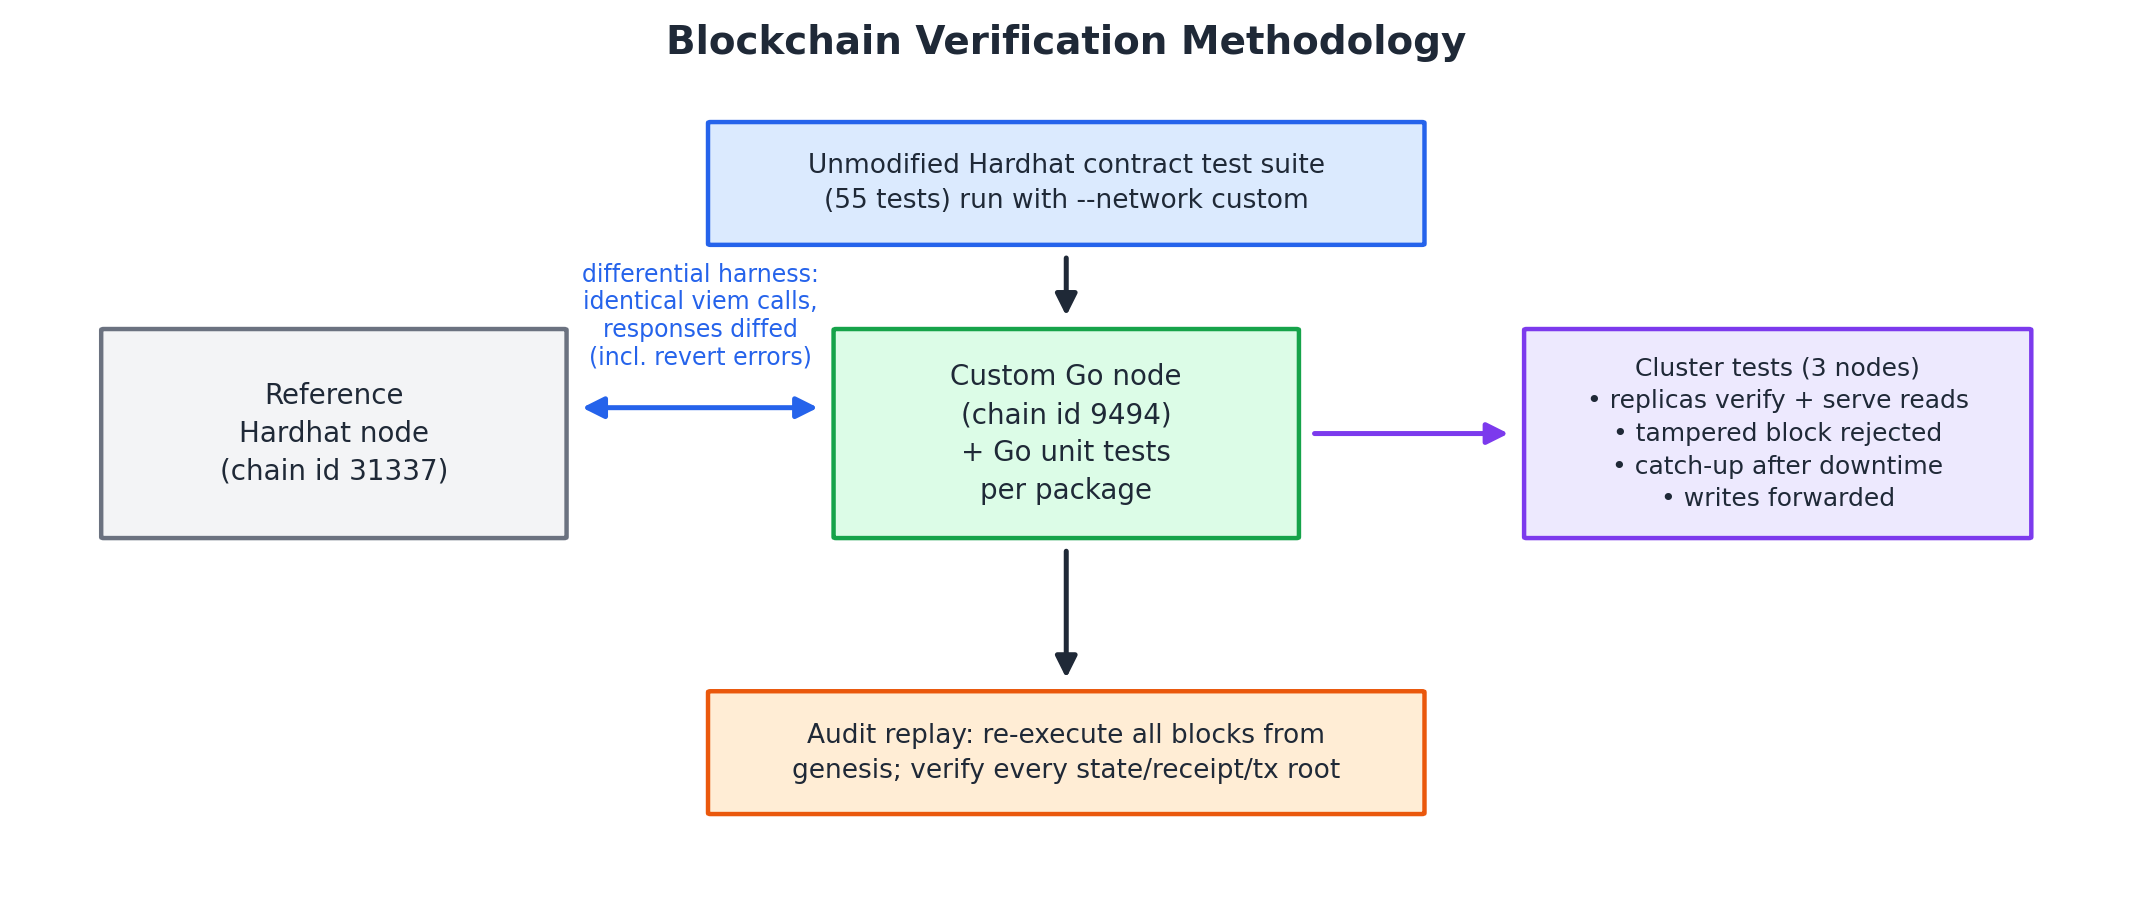
\includegraphics[width=0.92\textwidth]{Images/fig_chain_v2_testing.png}
\caption{Blockchain verification methodology: unit tests, differential testing against a reference Hardhat node, the unmodified contract test suite executed against the Go node, deterministic audit replay, and multi-node replication checks.}
\label{fig:chain-testing}
\end{figure}

\begin{enumerate}
    \item \textbf{Package-level unit tests} (Go) cover configuration validation, genesis determinism, transaction validation (nonce, chain id, gas cap), EVM execution, block sealing, receipt and log derivation, and restart recovery, with table-driven cases per package.
    \item \textbf{Differential testing.} A harness issues identical viem calls to a live Hardhat node and to our node, then diffs the JSON responses after normalizing legitimately volatile fields (hashes, timestamps). This covers read methods, write receipts, and---critically---\emph{error shapes}: a revert with \texttt{Voting\_\_WrongPhase} must decode to the same custom error on both backends, since the applications' error handling depends on it. Response-shape checks additionally run viem's own formatters over the node's JSON to catch field-level deviations.
    \item \textbf{The Hardhat contract suite against the node.} The strongest compatibility evidence: the same 55-test suite from Table~\ref{tab:test-distribution} is executed unmodified with \texttt{--network custom}, so every assertion written for the reference EVM must also hold on ours---including time manipulation via the \texttt{evm\_increaseTime} development methods.
    \item \textbf{Deterministic audit replay.} The standalone audit tool re-executes the full block history on a fresh state database and verifies every block's state root, receipt root, transaction root, and linkage; deliberately corrupted test fixtures are detected at the exact offending block.
    \item \textbf{Replication checks.} Three-node cluster scenarios verify that replicas re-execute and accept honest blocks, reject blocks with tampered state roots, catch up correctly after downtime, and transparently forward writes to the sequencer.
\end{enumerate}

\section{Performance Characteristics}

% TODO(before submission): replace design-derived figures in this section with
% measured values from the blockchain e2e benchmark run (docs/blockchain-v2, M14).

\subsection{Latency Analysis}

\begin{table}[H]
\centering
\caption{Expected operation latency by system layer.}
\label{tab:latency}
\begin{tabular}{|l|l|l|}
\hline
\textbf{Operation} & \textbf{Expected latency} & \textbf{Environment} \\
\hline
Commitment generation & $<$10 ms & Mobile (Poseidon, JS) \\
\hline
Voter registration (tx) & $<$0.5 s & Custom chain (auto-mine) \\
\hline
ZK proof generation & 15--25 s & Mobile WebView (WASM) \\
\hline
Vote transaction (incl.\ on-chain verify) & $<$1 s & Custom chain (EVM Honk verify) \\
\hline
Block finality & Immediate & 1 tx/block, no reorgs \\
\hline
Replica propagation & $<$1 s & mTLS push, LAN \\
\hline
National result query & tens of ms & View call (no gas) \\
\hline
Merkle path retrieval & $<$100 ms & API route over event logs \\
\hline
\end{tabular}
\end{table}

\begin{figure}[H]
\centering
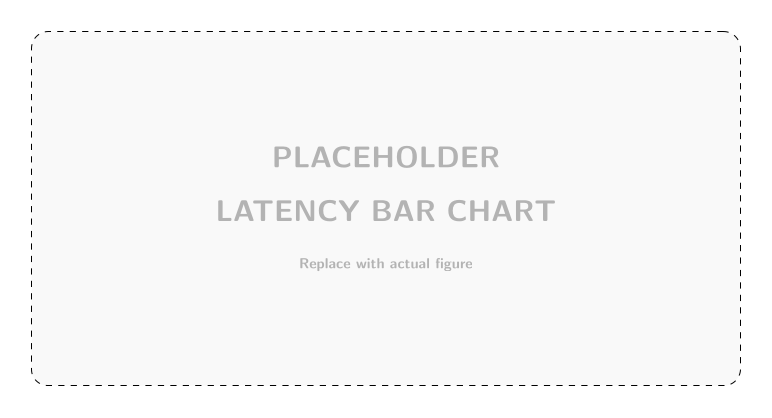
\includegraphics[width=0.85\textwidth]{Images/fig_latency_bar_chart.png}
\caption{Operation latency comparison: proof generation dominates the voter experience at 15--25 seconds; every on-chain step is sub-second.}
\label{fig:latency-chart}
\end{figure}

Because the node auto-mines one transaction per block with instant finality, there is no block-interval waiting time and no confirmation-depth heuristic: a transaction is final the moment its receipt exists.

\subsection{Throughput Analysis}

\begin{figure}[H]
\centering
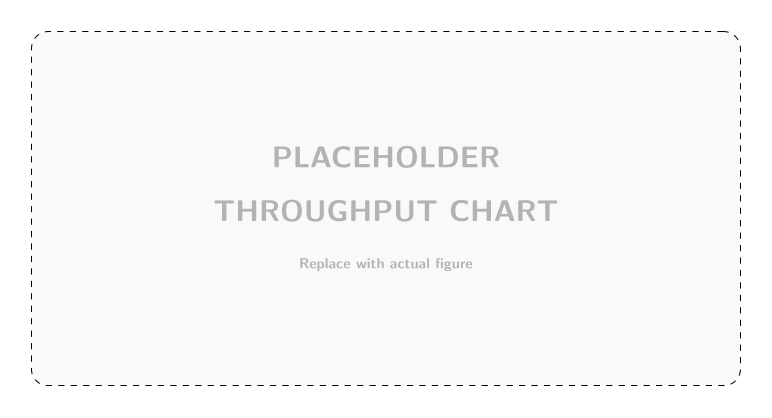
\includegraphics[width=0.85\textwidth]{Images/fig_throughput_chart.png}
\caption{System throughput by operation class: reads scale across replicas; vote throughput is bounded by on-chain proof verification.}
\label{fig:throughput}
\end{figure}

\begin{table}[H]
\centering
\caption{Expected throughput by operation class.}
\label{tab:throughput}
\begin{tabular}{|l|l|l|}
\hline
\textbf{Operation} & \textbf{Expected throughput} & \textbf{Bottleneck} \\
\hline
Registrations & Hundreds of tx/s & LeanIMT Merkle insert \\
\hline
Vote submissions & Tens of tx/s & On-chain Honk verification \\
\hline
Read queries & Thousands of req/s & Scales across read replicas \\
\hline
\end{tabular}
\end{table}

Vote throughput is the binding constraint: each vote executes the full UltraHonk verifier inside the EVM ($\sim$2M gas dominated by BN254 pairing operations), an order of magnitude more compute than any other transaction in the system. The multi-division architecture mitigates this naturally---divisions are independent contracts, and district-level node clusters can operate in parallel (Section~\ref{sec:scalability}).

\section{Gas Analysis}

\subsection{Per-Operation Gas Costs}

% TODO(before submission): replace approximations with the exact hardhat-gas-reporter
% output (packages/hardhat: REPORT_GAS=true yarn test).

\begin{table}[H]
\centering
\caption{Approximate gas consumption per smart contract operation.}
\label{tab:gas-costs}
\begin{tabular}{|l|l|l|}
\hline
\textbf{Operation} & \textbf{Gas (approx.)} & \textbf{Dominant Cost} \\
\hline
\texttt{register()} & 150K--600K & LeanIMT insert (Poseidon per level) \\
\hline
\texttt{vote()} & $\sim$2M & HonkVerifier.verify() pairing check \\
\hline
\texttt{setQuestion()} & $\sim$50K & String storage write \\
\hline
\texttt{setCandidates()} & $\sim$100K & Array storage writes \\
\hline
\texttt{startRegistration()} & $\sim$50K & Phase + deadline write \\
\hline
\texttt{createDivision()} & Several million & Full Voting.sol deployment \\
\hline
\end{tabular}
\end{table}

\texttt{register()} cost grows with tree depth: each LeanIMT insertion recomputes one Poseidon hash per level, so early registrations in a shallow tree are cheaper than late ones at the full depth of 16. The mobile client conservatively reserves 600K gas for registration and 15M for a vote---generous fixed limits chosen because gas is free on the custom chain, making tight estimation pointless.

\begin{figure}[H]
\centering
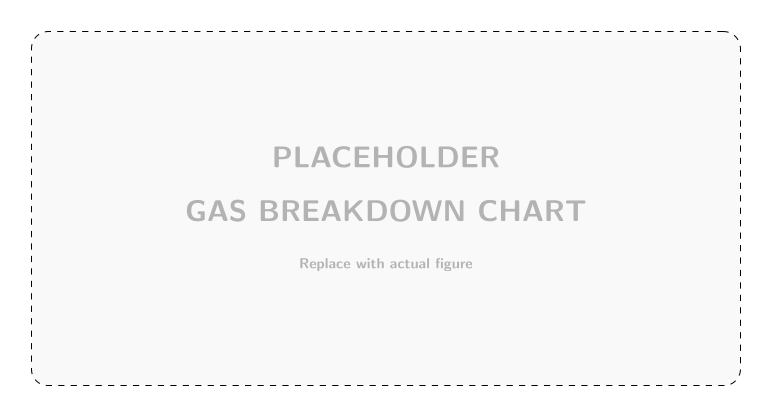
\includegraphics[width=0.85\textwidth]{Images/fig_gas_breakdown_chart.png}
\caption{Gas breakdown for the vote() function: ZK proof verification dominates, with roughly 90\% of the total spent inside HonkVerifier.verify().}
\label{fig:gas-breakdown}
\end{figure}

\subsection{Cost Comparison with Public Chains}

\begin{table}[H]
\centering
\caption{Order-of-magnitude cost if each vote ($\sim$2M gas) were paid at typical public-chain prices; exact figures vary with gas markets and token prices.}
\label{tab:cost-comparison}
\begin{tabular}{|l|l|l|}
\hline
\textbf{Chain} & \textbf{Per Vote} & \textbf{16M Voters} \\
\hline
Ethereum L1 & Tens of USD & Hundreds of millions USD \\
\hline
Optimistic / ZK rollups & \$0.01--\$1 & \$0.2M--\$16M \\
\hline
Polygon PoS & $<$\$0.01 & $<$\$0.2M \\
\hline
Custom chain (ours) & \textbf{\$0.00} & \textbf{\$0} \\
\hline
\end{tabular}
\end{table}

Beyond raw cost, public chains would also require distributing gas tokens to burner wallets---an operational nightmare and a deanonymization vector (the funding trail links a burner to whoever funded it). The gasless custom chain eliminates both problems structurally: a zero-balance burner submits its vote directly.

\section{Security Analysis}

\subsection{Attack-Defense Mapping}

\begin{figure}[H]
\centering
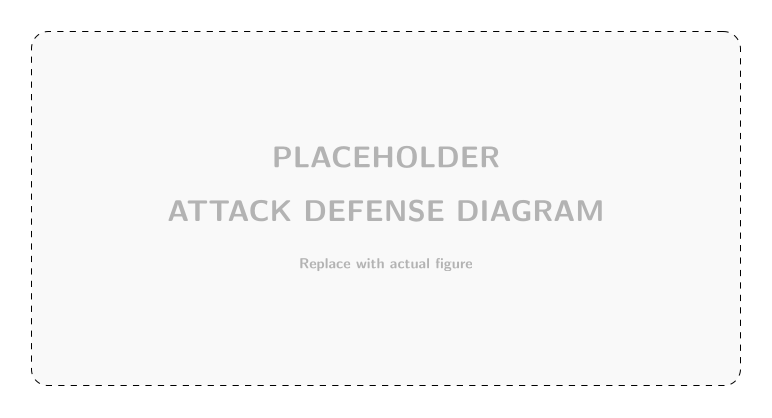
\includegraphics[width=0.85\textwidth]{Images/fig_attack_defense_diagram.png}
\caption{Attack-defense mapping: each potential attack vector and the corresponding defense mechanism.}
\label{fig:attack-defense}
\end{figure}

\begin{table}[H]
\centering
\caption{Security analysis: attack scenarios and defense effectiveness.}
\label{tab:security-analysis}
\resizebox{\textwidth}{!}{%
\begin{tabular}{|p{2.5cm}|p{3cm}|p{3.5cm}|l|p{3cm}|}
\hline
\textbf{Attack} & \textbf{Adversary} & \textbf{Defense} & \textbf{Result} & \textbf{Residual Risk} \\
\hline
Double voting & Voter & Nullifier uniqueness & Prevented & None (deterministic) \\
\hline
Impersonation & External & Biometric + hardware keystore & Prevented & Device theft + biometric \\
\hline
Ballot stuffing & External & ZK proof required & Prevented & None (soundness) \\
\hline
Vote buying & Coercer & Burner wallet & Mitigated & Screenshot before submit \\
\hline
Front-running & Node operator & Vote bound in proof & Prevented & None (cryptographic) \\
\hline
Sybil (multi-div) & Voter & NicRegistry (peppered hash) & Prevented & Fake NIC document \\
\hline
History tampering & Infrastructure & Replica re-execution + audit replay & Detected & Sequencer liveness (censorship is detectable) \\
\hline
Relay compromise & External/insider & Function whitelist + audit log; votes never pass through relay & Bounded & Lifecycle disruption (detectable); cannot forge votes \\
\hline
Admin fraud & Authority & Public verifiability & Detected & N/A (detectable) \\
\hline
Replay attack & External & Nullifier consumed & Prevented & None (one-time) \\
\hline
\end{tabular}%
}
\end{table}

Two rows deserve elaboration. \emph{History tampering}: the single sequencer cannot silently rewrite the record, because every replica re-executes every block and rejects state-root mismatches, and the offline audit tool re-derives the full election from genesis; what remains is a liveness risk (a malicious sequencer could stall or censor), which is externally observable. \emph{Relay compromise}: the administrative relay signs only whitelisted lifecycle functions and structurally cannot sign \texttt{register} or \texttt{vote}, so even full server compromise cannot manufacture or alter a single ballot.

\subsection{Coercion Resistance Analysis}

\begin{figure}[H]
\centering
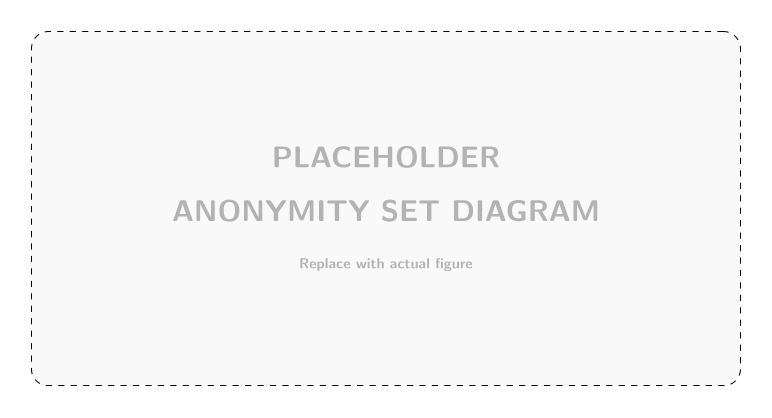
\includegraphics[width=0.85\textwidth]{Images/fig_anonymity_set_diagram.png}
\caption{Anonymity set visualization: a voter's ballot is indistinguishable among all registered voters in the division.}
\label{fig:anonymity-set}
\end{figure}

Our system provides \textbf{partial coercion resistance}:
\begin{itemize}
    \item \textbf{Protected against}: Post-vote coercion (voter cannot prove how they voted after the fact, as the burner wallet is discarded)
    \item \textbf{Vulnerable to}: Real-time coercion (adversary physically present during voting can observe the screen)
    \item \textbf{Mitigation}: The OTP step creates a time window; the actual proof generation and submission can be separated from candidate selection
\end{itemize}

Full coercion resistance would require re-voting capability (as in MACI) or deniable encryption---identified as future work.

\section{Comparison with Existing Systems}

\begin{table}[H]
\centering
\caption{Detailed comparison of our system with MACI, Semaphore, and Voatz.}
\label{tab:system-comparison-detail}
\resizebox{\textwidth}{!}{%
\begin{tabular}{|p{3.5cm}|l|l|l|l|}
\hline
\textbf{Property} & \textbf{Ours} & \textbf{MACI} & \textbf{Semaphore} & \textbf{Voatz} \\
\hline
Proof system & UltraHonk & Groth16 & Groth16 & None \\
\hline
Trusted setup & Universal SRS only & Yes (per-circuit) & Yes (universal) & N/A \\
\hline
Ballot privacy & ZK + burner & Encrypted & ZK proof & Server-side \\
\hline
Trusted coordinator & No & Yes & No & Yes \\
\hline
Gas cost per vote & \$0 (gasless) & $\sim$\$0.50 (L2) & $\sim$\$0.30 (L2) & N/A \\
\hline
Mobile proving & WebView WASM & Not supported & Not supported & N/A \\
\hline
Biometric auth & Hardware TEE & No & No & Central server \\
\hline
Multi-division & 160 divisions & Single election & Single group & Single election \\
\hline
Voter scalability & $\sim$10.5M & $\sim$10K & $\sim$65K & $\sim$1K (tested) \\
\hline
E2E verifiable & Yes & Yes & Partial & No \\
\hline
Double-vote prev. & Nullifier & Nullifier & Nullifier & Server-side \\
\hline
Sybil prevention & Hashed NIC & External & External & ID document \\
\hline
Coercion resistance & Partial & Full (re-vote) & None & None \\
\hline
Open source & Yes & Yes & Yes & No \\
\hline
\end{tabular}%
}
\end{table}

\section{Scalability Analysis}\label{sec:scalability}

\subsection{16 Million Voter Projection}

\begin{figure}[H]
\centering
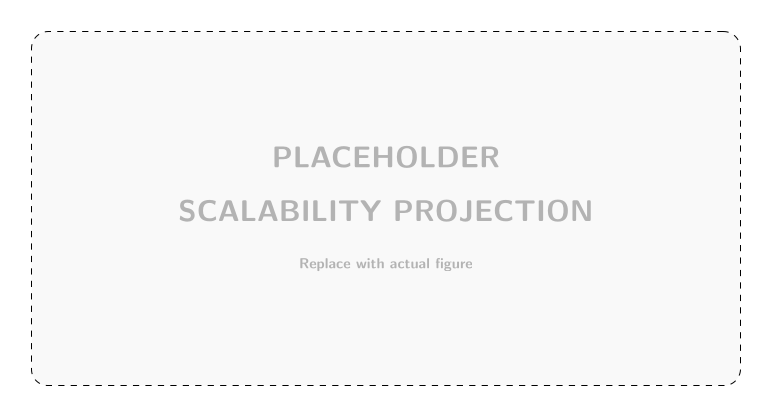
\includegraphics[width=0.85\textwidth]{Images/fig_scalability_projection.png}
\caption{Scalability projection: system capacity for Sri Lanka's 16 million voters across polling divisions.}
\label{fig:scalability}
\end{figure}

\begin{table}[H]
\centering
\caption{Scalability projection for national-scale deployment.}
\label{tab:scalability}
\begin{tabular}{|l|r|l|}
\hline
\textbf{Metric} & \textbf{Value} & \textbf{Calculation} \\
\hline
Total voters & 16,000,000 & Sri Lanka registered voters \\
\hline
Max voters per division & 65,536 & $2^{16}$ (fixed circuit depth of 16) \\
\hline
Capacity at 160 divisions & 10,485,760 & $160 \times 65{,}536$ \\
\hline
Divisions for 16M voters & 245 & $\lceil 16\text{M} / 65{,}536 \rceil$ \\
\hline
Voting window & 12 hours & Typical election day \\
\hline
Required national rate & $\sim$370 votes/sec & 16M / 43,200 s \\
\hline
Single-cluster vote rate & Tens/sec & On-chain Honk verification \\
\hline
\end{tabular}
\end{table}

The circuit never needs modification: capacity scales by \emph{adding divisions}, not by deepening the tree. The gap between the required national rate and a single cluster's vote throughput is closed by parallelism, which the architecture provides for free---divisions are fully independent contracts, so district-level chain clusters (each a sequencer with replicas, carrying a subset of divisions) can process votes concurrently, with the registry aggregation performed off-chain across clusters. Complementary future optimizations include proof batching and recursive aggregation (Chapter~\ref{ch:conclusion}).

\subsection{Storage Requirements}

\begin{table}[H]
\centering
\caption{Approximate storage requirements for a national-scale election.}
\label{tab:storage}
\begin{tabular}{|l|l|l|}
\hline
\textbf{Data} & \textbf{Per Item} & \textbf{16M Voters} \\
\hline
Commitments (Merkle leaves) & 32 bytes & 512 MB \\
\hline
Nullifier hashes & 32 bytes & 512 MB \\
\hline
Vote proofs (tx calldata) & $\sim$14 KB & $\sim$220 GB \\
\hline
Vote counts & 32 bytes/candidate & Negligible \\
\hline
Block overhead (headers, receipts) & $\sim$1 KB/block & $\sim$32 GB \\
\hline
\textbf{Total (order of magnitude)} & & $\sim$250 GB \\
\hline
\end{tabular}
\end{table}

The UltraHonk proof ($\sim$14~KB of calldata per vote) dominates storage. This is well within commodity-server capacity for a national election, and is naturally partitioned across district clusters. Proofs are verified at ingest---they are retained only to keep the full history independently re-executable by the audit tool.

\section{Circuit Correctness Verification}

\subsection{Test Vector Validation}

We generated deterministic test vectors and verified consistency across all system layers: the same input hashed by \texttt{poseidon-lite} in the browser/mobile JavaScript, by the Noir standard library's BN254 Poseidon inside the circuit, and by the \texttt{PoseidonT3} library on-chain must produce the identical field element.

\begin{table}[H]
\centering
\caption{Cross-layer test vector verification.}
\label{tab:test-vectors}
\begin{tabular}{|l|l|l|}
\hline
\textbf{Layer} & \textbf{Implementation} & \textbf{Result} \\
\hline
Browser / mobile & poseidon-lite (JS) & identical field element \\
\hline
Circuit & Noir stdlib \texttt{bn254::hash} & identical field element \\
\hline
On-chain & PoseidonT3 (Solidity) & identical field element \\
\hline
\end{tabular}
\end{table}

All three layers agree on every tested vector, confirming Poseidon parameterization consistency---a critical requirement that took three days to debug during development (see Chapter~\ref{ch:methodology}).

\section{End-to-End Flow Validation}\label{sec:e2e-flow}

The complete flow was validated repeatedly across backends: GN enrolls a voter (NIC hash reservation + allowlisting), the voter registers a commitment from the mobile app (OTP + biometric), generates a real UltraHonk proof in the WebView prover, and casts an anonymous vote from a fresh burner; results update live on the web dashboards, and the voter confirms inclusion via the nullifier-based ``Verify My Vote'' screen. Negative paths are asserted in the same runs: a second vote with the same nullifier is rejected with \texttt{Voting\_\_NullifierHashAlreadyUsed}, a stale Merkle root with \texttt{Voting\_\_InvalidRoot}, and out-of-phase actions with \texttt{Voting\_\_WrongPhase}. On the custom chain the same flow additionally proves the gasless property (the burner holds zero balance) and survives a node restart with full state recovery.

\section{Observations and Discussion}

\subsection{Proof Generation Time}

The 15--25 second proof generation time on mobile is the primary user experience bottleneck. While acceptable for a once-per-election action, this could be reduced to $<$5 seconds with native proving (Swoir/noir\_android)---identified as future work.

\subsection{Hermes Compatibility Trade-offs}

The Hermes BigInt limitation forced a WebView-based architecture for proof generation. While this adds complexity, it provides a clean separation between the UI layer (Hermes) and the cryptographic layer (system WebView with full BigInt support).

\subsection{Gas Efficiency}

The vote function's cost is dominated by proof verification: roughly 90\% of its $\sim$2M gas is spent inside \texttt{HonkVerifier.verify()} on BN254 pairing operations. On our gasless chain this cost is free to the voter but still bounds throughput. For any future public-L2 deployment it could be reduced by:
\begin{itemize}
    \item Batch verification (multiple proofs in one pairing check)
    \item Recursive proofs (aggregate many votes into one proof)
    \item Optimized verifier circuits
\end{itemize}

\subsection{Multi-Division Trade-offs}

The factory pattern provides excellent isolation and administrative delegation but introduces aggregation overhead: \texttt{getNationalResults()} iterates across all divisions, an $O(n)$ view call. For 160 divisions this is negligible (view calls are free and the results API caches them), but a deployment with thousands of divisions would move aggregation off-chain entirely.

\section{Summary}

Our comprehensive evaluation demonstrates:
\begin{enumerate}
    \item \textbf{Correctness}: All 55 contract unit tests pass---on the reference Hardhat network \emph{and} unmodified against the custom Go chain; cross-layer test vectors verify cryptographic consistency
    \item \textbf{Compatibility}: Differential testing shows the custom chain is JSON-RPC-indistinguishable from an Ethereum node for every operation the system performs
    \item \textbf{Performance}: Vote submission completes in $<$30 seconds end-to-end, dominated by mobile proof generation; on-chain steps are sub-second with instant finality
    \item \textbf{Security}: All identified attack vectors are either prevented cryptographically or rendered detectable through replication and audit replay
    \item \textbf{Scalability}: 10.5M voters at 160 divisions with no circuit modification; national scale reached by adding divisions and parallel district clusters
    \item \textbf{Cost}: Zero gas fees for voters (gasless chain), removing both the economic barrier and the funding-trail deanonymization vector
    \item \textbf{Privacy}: Formal voter--ballot unlinkability (Theorem~\ref{thm:unlinkability})
\end{enumerate}

\begin{figure}[H]
\centering
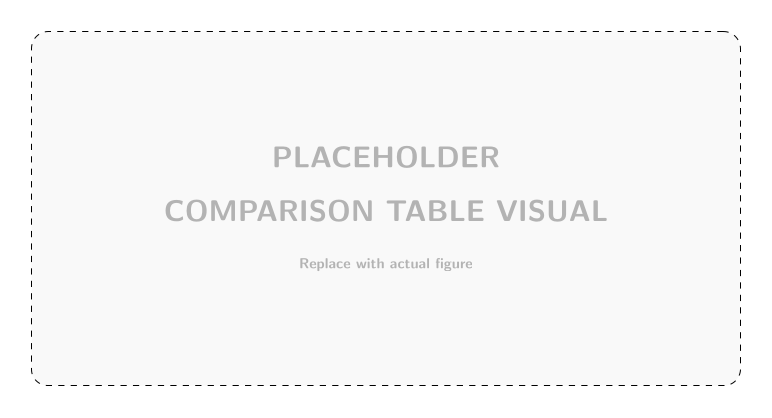
\includegraphics[width=0.85\textwidth]{Images/fig_comparison_table_visual.png}
\caption{Visual comparison summary: our system achieves the best combination of privacy, cost, and scalability among evaluated systems.}
\label{fig:comparison-visual}
\end{figure}

The system successfully demonstrates that privacy-preserving blockchain voting is feasible with current technology, though production deployment would require addressing the limitations identified in Chapter~\ref{ch:conclusion}.

\chapter{Conclusion and Future Work}\label{ch:conclusion}

This chapter summarizes the contributions of our work, evaluates achievement against stated objectives, acknowledges limitations, outlines future research directions, and provides concluding remarks on the broader impact of privacy-preserving blockchain voting.

\section{Summary of Contributions}

This project makes the following contributions to the field of electronic voting and applied cryptography:

\begin{enumerate}
    \item \textbf{First setup-free ZK voting system}: We demonstrate the first blockchain voting system using UltraHonk proofs that requires no trusted setup ceremony, eliminating a major deployment barrier for real-world elections.
    
    \item \textbf{Gasless sovereign blockchain}: We designed and implemented a custom Go blockchain embedding the Ethereum EVM that provides zero-cost voting---ensuring economic inclusivity for all citizens regardless of financial status.
    
    \item \textbf{Multi-division national architecture}: We modeled Sri Lanka's 160-division electoral structure with on-chain factory pattern deployment, GN officer delegation, cross-division Sybil prevention, and national result aggregation.
    
    \item \textbf{Mobile hardware-secured voting}: We implemented on-device ZK proof generation with hardware keystore protection, biometric authentication gates, and three-factor voter verification---a first for ZK voting systems.
    
    \item \textbf{Vote-binding ZK circuit}: We extended the Semaphore-style membership proof with vote-binding, where the candidate choice is cryptographically embedded in the proof, preventing front-running and vote modification attacks.
    
    \item \textbf{Five-layer fraud prevention}: We designed a defense-in-depth architecture combining identity gates, eligibility proofs, nullifier uniqueness, NIC de-duplication, and cryptographic binding---ensuring no single point of failure.
    
    \item \textbf{Comprehensive test suite}: We developed 54 unit tests covering all contract functions, phase transitions, access control, and adversarial scenarios, providing confidence in system correctness.
\end{enumerate}

\begin{figure}[H]
\centering
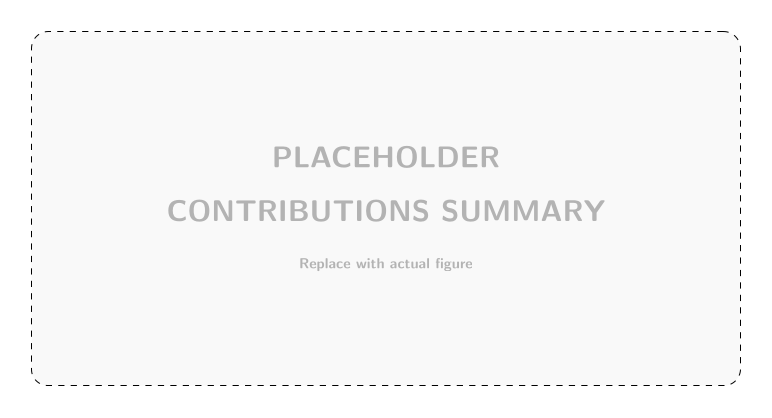
\includegraphics[width=0.85\textwidth]{Images/fig_contributions_summary.png}
\caption{Summary of project contributions mapped to the challenges they address in the e-voting landscape.}
\label{fig:contributions}
\end{figure}

\section{Achievement Against Objectives}

\begin{table}[H]
\centering
\caption{Evaluation of achievement against stated project objectives.}
\label{tab:objectives-eval}
\resizebox{\textwidth}{!}{%
\begin{tabular}{|c|p{5cm}|l|p{5cm}|}
\hline
\textbf{\#} & \textbf{Objective} & \textbf{Status} & \textbf{Evidence} \\
\hline
1 & Design ZK circuit proving voter membership without revealing identity & Achieved & Noir circuit with 4 constraints; UltraHonk proof verified on-chain \\
\hline
2 & Develop smart contracts with five layers of fraud prevention & Achieved & Voting.sol, ElectionRegistry, NicRegistry, HonkVerifier deployed and tested \\
\hline
3 & Build a custom gasless blockchain embedding the EVM & Achieved & Go blockchain with BoltDB, PBFT, REST API; executes same bytecode as Hardhat \\
\hline
4 & Develop mobile app with hardware security and on-device proving & Achieved & React Native (Expo 54); expo-secure-store; WebView bb.js WASM proving \\
\hline
5 & Implement web administration for EA and GN officers & Achieved & Next.js app with admin dashboard, GN portal, results page \\
\hline
6 & Model 160-division structure with national aggregation & Achieved & ElectionRegistry factory; \texttt{getNationalResults()} aggregation \\
\hline
7 & Achieve formal voter--ballot unlinkability & Achieved & Theorem~\ref{thm:unlinkability}: $\Pr[\mathcal{A} \to (\text{V}, \text{B})] \leq 1/|\mathcal{V}| + \text{negl}(\lambda)$ \\
\hline
\end{tabular}%
}
\end{table}

All seven project objectives have been achieved. The system demonstrates a complete, working prototype of a privacy-preserving electronic voting system with mathematical security guarantees.

\section{Limitations}

We acknowledge the following limitations of the current implementation:

\subsection{Ballot Secrecy}

Our system provides \textit{voter--ballot unlinkability} (no one can determine who cast which ballot) but not full \textit{ballot secrecy} (individual vote values are visible on-chain after counting). True ballot secrecy requires homomorphic tallying, where votes are encrypted and the tally is computed on ciphertexts without decrypting individual ballots. This is a fundamental limitation addressed in future work.

\subsection{Coercion Resistance}

While the burner wallet mechanism prevents post-hoc proof of vote, a physically present coercer can observe the voting screen in real-time. Full coercion resistance requires the ability to re-vote secretly (as in MACI) or deniable encryption schemes.

\subsection{Proof Generation Time}

The 15--25 second proof generation time on mobile, while acceptable for a once-per-election action, falls below the $<$5 second threshold expected for consumer applications. This is an engineering limitation (WASM execution in WebView) rather than a fundamental one.

\subsection{Trusted Ceremony for SRS}

While UltraHonk eliminates per-circuit trusted setup, it still uses a universal Structured Reference String (SRS) from the Aztec Ignition ceremony. In theory, if all ceremony participants collude, the soundness guarantee could be broken. In practice, the ceremony involved thousands of participants, making collusion computationally infeasible.

\subsection{Mobile Platform Limitations}

\begin{itemize}
    \item \textbf{iOS}: Face ID integration requires a custom development build (\texttt{NSFaceIDUsageDescription}); not tested in Expo Go
    \item \textbf{Root/jailbreak}: No detection implemented; a rooted device could potentially extract keystore secrets
    \item \textbf{Hermes BigInt}: The workaround (WebView proving) adds architectural complexity
\end{itemize}

\subsection{Production Readiness}

The system is a research prototype, not production-ready software. Gaps include:
\begin{itemize}
    \item No formal security audit by third-party experts
    \item No stress testing at 16M voter scale
    \item Development OTP provider (not production SMS gateway)
    \item No CI/CD pipeline or monitoring infrastructure
    \item No accessibility features (screen reader, high contrast, multi-language)
\end{itemize}

\section{Future Work}

\begin{figure}[H]
\centering
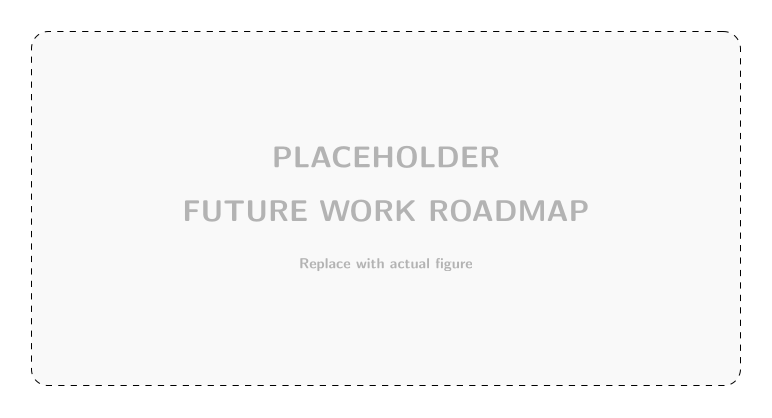
\includegraphics[width=0.85\textwidth]{Images/fig_future_work_roadmap.png}
\caption{Future work roadmap: short-term engineering improvements, medium-term protocol upgrades, and long-term research directions.}
\label{fig:future-roadmap}
\end{figure}

\subsection{Short-Term: Engineering Improvements}

\begin{enumerate}
    \item \textbf{Native ZK Proving}: Integrate Swoir (Noir's native mobile prover) or noir\_android to reduce proof generation from 15--25 seconds to $<$5 seconds. This eliminates the WebView architecture entirely.
    
    \item \textbf{Production OTP}: Replace the development OTP system with Firebase Authentication or Twilio for production-grade SMS verification with rate limiting and fraud detection.
    
    \item \textbf{ERC-4337 Paymaster}: For L2 deployment scenarios, implement an account abstraction paymaster that sponsors burner wallet gas fees without requiring a custom chain.
    
    \item \textbf{Root/Jailbreak Detection}: Integrate SafetyNet (Android) and App Attest (iOS) to prevent voting from compromised devices where keystore security guarantees are voided.
\end{enumerate}

\subsection{Medium-Term: Protocol Upgrades}

\begin{enumerate}
    \item \textbf{Homomorphic Tallying}: Implement additively homomorphic encryption (e.g., exponential ElGamal) where:
    \begin{equation}
    \text{Tally} = \text{Dec}\left(\prod_{i=1}^{n} \text{Enc}(v_i)\right) = \sum_{i=1}^{n} v_i
    \end{equation}
    This achieves full ballot secrecy---no entity ever sees individual decrypted votes. The tally is decrypted only in aggregate via threshold decryption among election commission nodes.
    
    \item \textbf{Re-Voting for Coercion Resistance}: Allow voters to submit multiple ballots (only the last counts), with the re-voting action hidden from observers. This requires encrypted ballot storage and a trusted coordinator to process the override logic---a trade-off between coercion resistance and trust minimization.
    
    \item \textbf{Formal Verification}: Verify the Noir circuit using automated theorem provers (Lean 4, Z3) to mathematically prove that:
    \begin{itemize}
        \item No valid proof can be generated without a valid witness
        \item The circuit faithfully implements the specified security properties
        \item No constraint under-specification allows exploits
    \end{itemize}
\end{enumerate}

\subsection{Long-Term: Research Directions}

\begin{enumerate}
    \item \textbf{Multi-Party Computation (MPC) Ceremony}: Conduct a public, verifiable MPC ceremony for the universal SRS, involving Sri Lankan institutions (universities, civil society, opposition parties) as participants. This provides transparent, auditable trust distribution.
    
    \item \textbf{Recursive Proofs for Scalability}: Use recursive proof composition (IVC/PCD) to aggregate thousands of individual vote proofs into a single proof, enabling $O(1)$ on-chain verification for the entire election:
    \begin{equation}
    \pi_{\text{aggregate}} = \text{Fold}(\pi_1, \pi_2, \ldots, \pi_n) \quad |\pi_{\text{aggregate}}| = O(1)
    \end{equation}
    
    \item \textbf{Post-Quantum Security}: Migrate from BN254 (vulnerable to quantum algorithms) to lattice-based proof systems (e.g., Plonky3 over Goldilocks field) that provide post-quantum security guarantees.
    
    \item \textbf{Decentralized Identity Integration}: Replace wallet-based voter identity with W3C Decentralized Identifiers (DIDs) and Verifiable Credentials, enabling interoperability with national digital identity systems.
    
    \item \textbf{Cross-Chain Interoperability}: Enable election result publication across multiple chains (Ethereum, Polygon, etc.) for maximum transparency and auditability by international observers.
\end{enumerate}

\section{Broader Impact}

This work demonstrates that the apparent conflict between voter privacy and election transparency can be resolved through modern cryptography. Zero-knowledge proofs enable a paradigm shift: from ``trust the authority'' to ``trust the mathematics.''

For Sri Lanka specifically, where election logistics cost millions of dollars and results take 24--48 hours to announce, a blockchain voting system could provide:
\begin{itemize}
    \item Instant results (tallies update in real-time)
    \item Zero logistical cost for ballot transport and counting
    \item Accessibility for overseas citizens and disabled voters
    \item Mathematical proof of election integrity (no recounts needed)
    \item Reduced human error in counting and tabulation
\end{itemize}

\section{Concluding Remarks}

We have presented a complete, working implementation of a privacy-preserving electronic voting system that combines zero-knowledge proofs, a custom blockchain, hardware-secured mobile authentication, and multi-division national architecture. Our system achieves formal voter--ballot unlinkability without requiring any trusted third party---a property that no prior deployed system has accomplished.

The journey from initial concept to working prototype involved four circuit iterations, three contract architecture generations, and numerous integration challenges (Poseidon field mismatches, Hermes BigInt limitations, EVM precompile registration). Each failure taught us something essential about the intersection of theoretical cryptography and practical engineering.

While significant work remains before production deployment---particularly homomorphic tallying, native proving, and formal verification---this project establishes that the fundamental architecture is sound and implementable with current technology. The combination of UltraHonk (no trusted setup), a custom gasless chain (economic inclusivity), and hardware-backed mobile security (physical presence verification) represents a viable path toward truly private, truly verifiable, and truly accessible democratic elections.

\vspace{1cm}

\begin{quote}
\textit{``The ballot is stronger than the bullet.''} --- Abraham Lincoln

\vspace{0.3cm}

We add: \textit{``And a zero-knowledge proof is stronger than both---for it proves truth without revealing secrets.''}
\end{quote}



%%%%%%%%%%%%%%%%%%%%% The End matters %%%%%%%%%%%%%%%%%%%%%

\begin{appendix}
\chapter{Source Code Listings}\label{app:source}

This appendix contains the complete source code of the critical system components.

\section{ZK Circuit --- main.nr}

\begin{lstlisting}[caption={Complete Noir ZK circuit (packages/circuits/src/main.nr)}]
use std::hash::poseidon::bn254::hash_1;
use std::hash::poseidon::bn254::hash_2;
use binary_merkle_root::binary_merkle_root;

fn main(
    // public inputs
    nullifier_hash: pub Field,
    // private inputs
    nullifier: Field,
    secret: Field,
    // public inputs
    root: pub Field,
    vote: pub Field,
    depth: pub u32,
    // private inputs
    index: Field,
    // max of 2^16 leaves --> 65536 leaves
    siblings: [Field; 16],
) {
    // Recompute nullifier_hash and verify it matches the public input
    let computed_nullifier_hash: Field = hash_1([nullifier]);
    assert(computed_nullifier_hash == nullifier_hash);

    // Compute the commitment (leaf of the Merkle tree)
    let commitment: Field = hash_2([nullifier, secret]);

    // Count the non-zero siblings to determine the actual path length
    let mut siblings_num = 0;
    for i in 0..siblings.len() {
        if siblings[i] != 0 {
            siblings_num += 1;
        }
    }
    // Ensure depth doesn't exceed the fixed array length
    assert(depth <= siblings.len());

    // Convert leaf index to little-endian bits for path traversal
    let index_bits: [u1; 16] = index.to_le_bits();

    // Recompute the Merkle root from the commitment and siblings
    let computed_root = binary_merkle_root(
        hash_2, commitment, siblings_num, index_bits, siblings
    );

    // Assert the computed root matches the on-chain root
    assert(computed_root == root);

    // Bind the vote to the proof and range-check to 8 bits (0..=255)
    let _vote_bits: [u1; 8] = vote.to_le_bits();
}
\end{lstlisting}

\section{Smart Contract --- Voting.sol (Key Functions)}

\begin{lstlisting}[caption={Voting.sol --- Registration function}]
function register(uint256 _commitment)
    external inPhase(Phase.Registration)
{
    uint256 electionId = s_electionId;
    if (!s_voters[electionId][msg.sender] ||
         s_hasRegistered[electionId][msg.sender])
        revert Voting__NotAllowedToVote();
    if (s_commitments[electionId][_commitment])
        revert Voting__CommitmentAlreadyAdded(_commitment);
    s_commitments[electionId][_commitment] = true;
    s_hasRegistered[electionId][msg.sender] = true;
    s_trees[electionId].insert(_commitment);
    emit NewLeaf(s_trees[electionId].size - 1, _commitment);
}
\end{lstlisting}

\begin{lstlisting}[caption={Voting.sol --- Vote function with ZK verification}]
function vote(
    bytes memory _proof,
    bytes32 _nullifierHash,
    bytes32 _root,
    bytes32 _vote,
    bytes32 _depth
) external inPhase(Phase.Voting) {
    uint256 electionId = s_electionId;
    if (_root == bytes32(0)) revert Voting__EmptyTree();
    if (_root != bytes32(s_trees[electionId].root()))
        revert Voting__InvalidRoot();

    uint256 candidateIdx = uint256(_vote);
    if (candidateIdx >= s_candidates.length)
        revert Voting__InvalidCandidate(candidateIdx);

    bytes32[] memory publicInputs = new bytes32[](4);
    publicInputs[0] = _nullifierHash;
    publicInputs[1] = _root;
    publicInputs[2] = _vote;
    publicInputs[3] = _depth;

    if (!i_verifier.verify(_proof, publicInputs))
        revert Voting__InvalidProof();

    if (s_nullifierHashes[electionId][_nullifierHash])
        revert Voting__NullifierHashAlreadyUsed(_nullifierHash);
    s_nullifierHashes[electionId][_nullifierHash] = true;

    uint256 newCount = ++s_voteCounts[electionId][candidateIdx];
    emit VoteCast(_nullifierHash, msg.sender,
                  candidateIdx, block.timestamp, newCount);
}
\end{lstlisting}

\begin{lstlisting}[caption={Voting.sol --- Phase management}]
enum Phase { Setup, Registration, Voting, Ended }

modifier inPhase(Phase expected) {
    _maybeAdvancePhase();
    if (s_phase != expected)
        revert Voting__WrongPhase(expected, s_phase);
    _;
}

function _maybeAdvancePhase() internal {
    if (s_phase == Phase.Registration &&
        block.timestamp >= s_registrationEndTime) {
        s_phase = Phase.Ended;
        emit PhaseChanged(Phase.Ended, block.timestamp);
    } else if (s_phase == Phase.Voting &&
               block.timestamp >= s_votingEndTime) {
        s_phase = Phase.Ended;
        emit PhaseChanged(Phase.Ended, block.timestamp);
    }
}

function startRegistration(uint256 _durationSec)
    external onlyOwner inPhase(Phase.Setup)
{
    if (_durationSec == 0) revert Voting__InvalidDuration();
    if (s_candidates.length == 0) revert Voting__NoCandidates();
    s_phase = Phase.Registration;
    s_registrationEndTime = block.timestamp + _durationSec;
    emit PhaseChanged(Phase.Registration, s_registrationEndTime);
}
\end{lstlisting}

\section{Smart Contract --- ElectionRegistry.sol}

\begin{lstlisting}[caption={ElectionRegistry.sol --- Division factory and aggregation}]
contract ElectionRegistry is Ownable {
    struct Division {
        string name;
        address votingContract;
        address gnOfficer;
        bool active;
    }

    Division[] public divisions;
    address public immutable i_verifier;

    constructor(address _owner, address _verifier)
        Ownable(_owner) {
        i_verifier = _verifier;
    }

    function createDivision(string calldata _name)
        external onlyOwner
        returns (uint256 divisionId, address votingContract)
    {
        string[] memory emptyCandidates = new string[](0);
        Voting newVoting = new Voting(
            owner(), i_verifier, "", emptyCandidates);
        votingContract = address(newVoting);
        divisionId = divisions.length;
        divisions.push(Division({
            name: _name,
            votingContract: votingContract,
            gnOfficer: address(0),
            active: true
        }));
        emit DivisionCreated(divisionId, _name, votingContract);
    }

    function getNationalResults()
        external view returns (uint256[] memory totals)
    {
        if (divisions.length == 0) return totals;
        string[] memory candidates =
            IVotingView(divisions[0].votingContract)
            .getCandidates();
        totals = new uint256[](candidates.length);
        for (uint256 i = 0; i < divisions.length; i++) {
            if (divisions[i].active) {
                for (uint256 c = 0; c < candidates.length; c++) {
                    totals[c] += IVotingView(
                        divisions[i].votingContract
                    ).getVoteCount(c);
                }
            }
        }
    }
}
\end{lstlisting}

\section{Smart Contract --- NicRegistry.sol}

\begin{lstlisting}[caption={NicRegistry.sol --- Cross-division Sybil prevention}]
contract NicRegistry is Ownable {
    error NicRegistry__AlreadyUsed(bytes32 nicHash);

    mapping(bytes32 => bool) private usedNicHashes;
    mapping(address => bool) private s_votingContracts;

    modifier onlyOwnerOrGN(address votingContract) {
        require(s_votingContracts[votingContract],
                "Unregistered division");
        require(
            msg.sender == owner() ||
            msg.sender == IVotingGN(votingContract)
                         .s_gnOfficer(),
            "Not owner or GN");
        _;
    }

    function reserveNicHash(
        bytes32 nicHash, address votingContract
    ) external onlyOwnerOrGN(votingContract)
      returns (bool) {
        if (usedNicHashes[nicHash])
            revert NicRegistry__AlreadyUsed(nicHash);
        usedNicHashes[nicHash] = true;
        emit NicHashReserved(nicHash);
        return true;
    }
}
\end{lstlisting}

\section{Mobile Services --- Keystore (keystore.ts)}

\begin{lstlisting}[caption={Hardware-backed key storage service}]
import * as SecureStore from 'expo-secure-store';
import { generatePrivateKey, privateKeyToAddress }
    from 'viem/accounts';

const AUTH_OPTIONS: SecureStore.SecureStoreOptions = {
  requireAuthentication: !__DEV__,
  authenticationPrompt: "Unlock your voting identity",
  keychainAccessible:
    SecureStore.WHEN_UNLOCKED_THIS_DEVICE_ONLY,
};

export async function createIdentity(): Promise<string> {
  const pk = generatePrivateKey();
  const addr = privateKeyToAddress(pk);
  await SecureStore.setItemAsync(
    'slvote.privateKey', pk, AUTH_OPTIONS);
  await SecureStore.setItemAsync('slvote.address', addr);
  return addr;
}

export async function getPrivateKey(): Promise<string> {
  // Triggers biometric prompt
  return await SecureStore.getItemAsync(
    'slvote.privateKey', AUTH_OPTIONS);
}

export async function getVoterSecrets() {
  const n = await SecureStore.getItemAsync(
    'slvote.nullifier', AUTH_OPTIONS);
  const s = await SecureStore.getItemAsync(
    'slvote.secret', AUTH_OPTIONS);
  return n && s ? { nullifier: n, secret: s } : null;
}
\end{lstlisting}

\section{Mobile Services --- Chain Interaction (chain.ts)}

\begin{lstlisting}[caption={Legacy transaction signing for Hermes compatibility}]
import { createWalletClient, http, encodeFunctionData }
    from 'viem';
import { privateKeyToAccount } from 'viem/accounts';

export async function submitVote(
  contractAddr: string,
  callData: VoteCallData,
  burnerKey: string
) {
  const account = privateKeyToAccount(burnerKey);
  const nonce = await publicClient.getTransactionCount({
    address: account.address
  });
  const gasPrice = await publicClient.getGasPrice();

  // Manual legacy tx (Hermes EIP-1559 incompatible)
  const signedTx = await account.signTransaction({
    to: contractAddr,
    data: encodeFunctionData({
      abi: VotingABI,
      functionName: 'vote',
      args: [callData.proof, callData.nullifierHash,
             callData.root, callData.vote, callData.depth]
    }),
    nonce,
    gasPrice,
    gas: 500000n,
    type: 'legacy',
  });

  return await publicClient.sendRawTransaction({
    serializedTransaction: signedTx
  });
}

export function newBurnerAccount() {
  const pk = generatePrivateKey();
  return {
    privateKey: pk,
    address: privateKeyToAddress(pk)
  };
}
\end{lstlisting}

\chapter{Test Results and Deployment Outputs}\label{app:tests}

\section{Smart Contract Test Output}

\begin{lstlisting}[caption={Complete Hardhat test suite output (54 tests passing)}]
  Voting Contract
    Setup Phase
      + should start in Setup phase
      + should allow owner to set question
      + should reject setQuestion outside Setup
      + should allow setting candidates
      + should reject > 100 candidates
      + should reject empty candidate list
      + should reject startRegistration with 0 duration
      + should allow owner to set GN officer

    Registration Phase
      + allowlisted voter can register commitment
      + registration status updates correctly
      + tree root changes after registration
      + tree depth changes with multiple registrations
      + emits NewLeaf with correct index
      + rejects non-allowlisted voter
      + rejects already-registered voter
      + rejects duplicate commitment
      + rejects registration during Voting phase
      + multiple voters can register sequentially
      + tree size matches registration count
      + emits VoterAdded events

    Phase Transitions
      + startVoting transitions Registration -> Voting
      + auto-advances Registration -> Ended after deadline
      + auto-advances Voting -> Ended after deadline
      + owner can endElection early
      + non-owner cannot call startVoting
      + non-owner cannot call endElection

    Voting Phase (with mock verifier)
      + valid proof accepted, tally incremented
      + reused nullifier rejected
      + invalid proof rejected
      + invalid candidate index rejected
      + stale root rejected

    View Functions
      + getVotingData returns correct structure
      + getVoteCounts returns zeros initially
      + getVoterData reports correctly
      + currentPhase reflects elapsed deadlines
      + isNullifierUsed returns correct state

    Reset / Multi-Election
      + resetElection returns to Setup
      + election ID bumps after reset
      + ElectionReset event emitted

  GN Officer and Registry
    GN Officer Management
      + owner can set GN officer
      + non-owner cannot set GN officer
      + GN can add voters during Setup
      + GN cannot add voters during Registration
      + non-GN cannot add voters
      + GN cannot add voters during Voting
      + owner can still add voters

    Election Registry
      + owner can add a division
      + non-owner cannot add division
      + getDivisionCount returns correct count
      + getAllDivisions returns correct data
      + getNationalVoteCount aggregates correctly
      + owner can update division

  NIC Registry
    + owner can set voting contract authorization
    + GN can reserve NIC hash
    + duplicate NIC hash reverts
    + unauthorized caller reverts
    + non-registered division reverts

  54 passing (5s)
\end{lstlisting}

\section{Gas Usage Report}

\begin{lstlisting}[caption={Gas usage per operation (Hardhat gas reporter)}]
|  Contracts / Methods    |  Min      |  Max      |  Avg      |
|-------------------------|-----------|-----------|-----------|
|  NicRegistry            |           |           |           |
|    reserveNicHash       |  50,228   |  55,553   |  54,222   |
|    setVotingContract    |     -     |     -     |  47,807   |
|  Voting                 |           |           |           |
|    addVoters            |  53,922   |  78,607   |  77,940   |
|    endElection          |     -     |     -     |  32,784   |
|    register             | 149,833   | 189,006   | 157,178   |
|    resetElection        |  65,295   |  67,535   |  65,575   |
|    setCandidates        |     -     |     -     | 125,481   |
|    setGNOfficer         |     -     |     -     |  47,305   |
|    setQuestion          |     -     |     -     |  51,051   |
|    startRegistration    |     -     |     -     |  72,222   |
|    startVoting          |     -     |     -     |  55,125   |
|  Deployments            |           |  Gas Used |  % Limit  |
|  HonkVerifier           |     -     | 4,726,613 |  29.5%    |
|  LeanIMT                | 1,028,149 | 1,028,221 |   6.4%    |
|  NicRegistry            |     -     |   337,595 |   2.1%    |
|  PoseidonT3             |     -     | 3,695,091 |  23.1%    |
|  Voting                 | 1,990,930 | 2,016,450 |  12.4%    |
\end{lstlisting}

\section{Deployment Output (3 Division Demo)}

\begin{lstlisting}[caption={Multi-division deployment output}]
deploying "PoseidonT3" ... deployed at
    0x5FbDB2315678afecb367f032d93F642f64180aa3
    with 3,695,091 gas
deploying "LeanIMT" ... deployed at
    0xe7f1725E7734CE288F8367e1Bb143E90bb3F0512
    with 1,028,221 gas
deploying "HonkVerifier" ... deployed at
    0x9fE46736679d2D9a65F0992F2272dE9f3c7fa6e0
    with 4,726,613 gas
deploying "Voting" ... deployed at
    0xCf7Ed3AccA5a467e9e704C703E8D87F634fB0Fc9
    with 1,991,182 gas
deploying "ElectionRegistry" ... deployed at
    0xDc64a140Aa3E981100a9becA4E685f962f0cF6C9
    with 3,390,808 gas
deploying "NicRegistry" ... deployed at
    0x5FC8d32690cc91D4c39d9d3abcBD16989F875707
    with 337,595 gas

Multi-division election deployed:
  Registry: 0xDc64a140Aa3E981100a9becA4E685f962f0cF6C9
  NicRegistry: 0x5FC8d32690cc91D4c39d9d3abcBD16989F875707
  Divisions: 3
  Candidates: Anura Kumara Dissanayake (NPP),
              Sajith Premadasa (SJB),
              Ranil Wickremesinghe (UNP)
  GN Kaduwela:  0xf39Fd6e51aad88F6F4ce6aB8827279cffFb92266
  GN Colombo:   0x3C44CdDdB6a900fa2b585dd299e03d12FA4293BC
  GN Gampaha:   0x90F79bf6EB2c4f870365E785982E1f101E93b906
\end{lstlisting}

\section{Mobile App Build Output}

\begin{lstlisting}[caption={Expo export output confirming successful build}]
$ npx expo export --platform android --output-dir dist

  android bundles (1):
  _expo/static/js/android/
    entry-f3d281ff2509f8797675dea470443ce1.hbc (5.69 MB)

  Files (1):
  metadata.json (1.81 kB)

Exported: dist
\end{lstlisting}

\section{TypeScript Compilation}

\begin{lstlisting}[caption={Zero TypeScript errors across all packages}]
$ npx tsc --noEmit
# (no output = 0 errors)

$ npx expo export --platform android
# Successfully exported (confirms type safety)
\end{lstlisting}

\end{appendix}

%% ____BIBLIOGRAPHY____%%
\bibliographystyle{ieeetr}
\bibliography{bibliography}
\addcontentsline{toc}{chapter}{Bibliography}

\end{document}

\addcontentsline{toc}{chapter}{APPENDIX}

%%%%%%%%%%%%%%%%%%%%% Bibiliography %%%%%%%%%%%%%%%%%%%%%
\cleardoublepage
\bibliographystyle{ieeetr}
\refstepcounter{chapter}
\addcontentsline {toc}{chapter}{\bibname}
% _____Add Bibiliography using BibTex file_____
\bibliography{bibliography} 

\end{document}
